% STEP 1: Choose oneside or twoside. Use the 'draft' option a lot when writing.
\documentclass[english, oneside]{HYgradu}

\usepackage[utf8]{inputenc} % For UTF8 support. Use UTF8 when saving your file.
\usepackage{lmodern} % Font package
\usepackage{textcomp}
\usepackage[pdftex]{color, graphicx} % For pdf output and jpg/png graphics
\usepackage[pdftex, plainpages=false]{hyperref} % For hyperlinks and pdf metadata
\usepackage{fancyhdr} % For nicer page headers
%\usepackage{tikz} % For making vector graphics (hard to learn but powerful)
%\usepackage{wrapfig} % For nice text-wrapping figures (use at own discretion)
\usepackage{amsmath, amssymb} % For better math
\usepackage[sort,colon]{natbib} % For bibliography
\usepackage[bf]{caption} % For more control over figure captions
\usepackage{marginnote} % margin notes for myself
%\usepackage{svg} % vector graphics
\usepackage{graphicx}
\graphicspath{{kuvat/tex/}}
\usepackage{wasysym}
\usepackage{tabularx}
\usepackage{adjustbox}
\usepackage{makecell}
\usepackage{rotating}
\usepackage[shortcuts]{extdash}
\usepackage{physics}
\usepackage[super]{nth}

% titlesec and fix for no numbering on titlesec 2.10.2
\usepackage{titlesec}
\usepackage{etoolbox}
\makeatletter
\patchcmd{\ttlh@hang}{\parindent\z@}{\parindent\z@\leavevmode}{}{}
\patchcmd{\ttlh@hang}{\noindent}{}{}{}
\makeatother

\fussy % Probably not needed but you never know...

\renewcommand{\topfraction}{.75} % less single-float pages
\renewcommand{\floatpagefraction}{.75} % less single-float pages

\newcommand{\matr}[1]{\mathbf{#1}}

% näillä subsubsubsection käyttöön
%\titleclass{\subsubsubsection}{straight}[\subsection]
%\newcounter{subsubsubsection}[subsubsection]
%\renewcommand\thesubsubsubsection{\thesubsection.\arabic{subsubsubsection}}
%\titleformat{\subsubsubsection}
%  {\normalfont\normalsize\bfseries}{\thesubsubsubsection}{1em}{}
%\titlespacing*{\subsubsubsection}
%{0pt}{3.25ex plus 1ex minus .2ex}{1.5ex plus .2ex}
%\makeatletter
%\def\toclevel@subsubsubsection{3}
%\def\l@subsubsubsection{\@dottedtocline{4}{7em}{4em}}
%\@addtoreset{subsubsubsection}{section}
%\@addtoreset{subsubsubsection}{subsection}
%\makeatother
%\setcounter{secnumdepth}{3}
%\setcounter{tocdepth}{4}

% OPTIONAL STEP: Set up properties and metadata for the pdf file that pdfLaTeX makes.
% But you don't really need to do this unless you want to.
%\hypersetup{
%    bookmarks=true,         % show bookmarks bar first?
%    unicode=true,           % to show non-Latin characters in Acrobat’s bookmarks
%    pdftoolbar=true,        % show Acrobat’s toolbar?
%    pdfmenubar=true,        % show Acrobat’s menu?
%    pdffitwindow=false,     % window fit to page when opened
%    pdfstartview={FitH},    % fits the width of the page to the window
%    pdftitle={},            % title
%    pdfauthor={},           % author
%    pdfsubject={},          % subject of the document
%    pdfcreator={},          % creator of the document
%    pdfproducer={pdfLaTeX}, % producer of the document
%    pdfkeywords={something} {something else}, % list of keywords for
%    pdfnewwindow=true,      % links in new window
%    colorlinks=true,        % false: boxed links; true: colored links
%    linkcolor=black,        % color of internal links
%    citecolor=black,        % color of links to bibliography
%    filecolor=magenta,      % color of file links
%    urlcolor=cyan           % color of external links
%}

% STEP 2:
% Set up all the information for the title page and the abstract form.
% Replace parameters with your information.
\title{Your Title Here}
\author{Anni Järvenpää}
\date{\today}
\level{Master's thesis}
\faculty{Faculty of Science}
\department{Department of Physics}
\address{PL 64 (Gustaf Hällströmin katu 2a)\\00014 University of Helsinki}
\subject{Astronomy}
\prof{Dr. Till Sawala}{Professor Peter Johansson}
\censors{prof. Smith}{doc. Smythe}{}
\depositeplace{}
\additionalinformation{}
\numberofpagesinformation{\numberofpages\ pages}
\classification{}
\keywords{Your keywords here}
\quoting{}%``Bachelor's degrees make pretty good placemats if you get them laminated.'' \\---Jeph Jacques}
% There is a way out of every box, a solution to every puzzle; it's just a matter of finding it
% Things are only impossible until they're not

\begin{document}

% Generate title page.
\maketitle
% STEP 3:
% Write your abstract (of course you really do this last).
% You can make several abstract pages (if you want it in different languages),
% but you should also then redefine some of the above parameters in the proper
% language as well, in between the abstract definitions.

\begin{abstract}
Abstract goes here.
\end{abstract}

% Place ToC
\mytableofcontents

% set line spacing to the publication-ready single spacing:
%\singlespacing
%\onehalfspacing

% -----------------------------------------------------------------------------------
% STEP 4: Write the thesis.
% Your actual text starts here. You shouldn't mess with the code above the line except
% to change the parameters. Removing the abstract and ToC commands will mess up stuff.
\chapter{Introduction}

\section{TL;DR version of prerequisite information}
\begin{enumerate}
	\item galaxies form
	\begin{itemize}
		\item Why?
		\item When?
		\item How?
		\item Where?
	\end{itemize}
	\item galaxies form in groups
	\item our local group is one of these
	\item something about large scale distribution of galaxies
\end{enumerate}

\section{History of Local Group Research}
LG objects visible with naked eye -> realization they are something outside our galaxy -> realization they are something very much like our galaxy

First determining distance was difficult, now mass is more interesting question

\section{Aim of This Thesis}
Whatever the main results end up being, presented in somewhat coherent manner and hopefully sugar-coated enough to sound Important and Exciting.


\chapter{Theoretical Background}
%Think whether LG or LCDM first
%theorythingies from Fattahi paper introduction

Cosmology determines the properties of the Universe, including its origin, the rules by which it evolves and the structures that arise within it \citep{mo2010galaxy}. Thus many fields of astronomy and astrophysics, including the study of galaxies and galaxy groups such as the Local Group and its members, are tightly connected to the study of cosmology. This section gives a brief explanation of the current cosmological understanding, its relevant implications and how the Local Group is currently viewed in ta cosmological context.

\section{Basics of Cosmology}
Understanding processes that take place on very large scales or take long times requires understanding some basic cosmology. The following sections will cover the most basic concepts of cosmology, the evolution of the Universe on both large and small scales, and the $\Lambda$CDM model which is currently the cosmological model that best matches the observations on multiple scales \citep{mo2010galaxy}. Sections \ref{universe-evolution} and \ref{universe-composition} cover large scales at which the cosmological principle applies and section \ref{universe-structure} covers smaller scales of individual dark matter haloes.

\subsection{Evolution of the Universe} \label{universe-evolution}
%\\- FRW
%\\- - cosmological principle
%\\- - fundamental observer
%\\- - radial expansion/contraction
%\\- - Friedmann equations
%\\- - critical density
%\\- - density parameters
%\\- - cosmic time
%\\- - (3D hypersurface, ds)
%\\- - a, K
%\\- - proper vs comoving distances
%\\- - H(t)
%\\- - redshift
%\\- - peculiar + expansion = proper velocity
%\\- - Values of the density parameters (how much matter, dm, radiation, lambda is there?)

The current cosmological understanding is based on a subset of the general theory of relativity together with simple hypotheses such as the cosmological principle, which states that on large scales the Universe is spatially homogeneous and isotropic \citep{mo2010galaxy}. At a given location, an observer might not see this, as is easy to understand when considering two observers located at the same point but moving relative to each other. In this situation, it is  clear that at least one of the observers will see a dipole in the surrounding velocities and thus will not observe the universe to be isotropic. Nonetheless, in an isotropic universe, for every point in space we can define a so-called fundamental observer as the observer who sees the universe as isotropic \citep{mo2010galaxy}. These fundamental observers correspond to a cosmological rest frame, which can be determined at a given location e.g. by observing the cosmic microwave background and subtracting the velocity corresponding to the observed dipole component \citep{mo2010galaxy}.

The existence of such fundamental observers has interesting consequences. The existence of any large-scale flows is clearly prohibited, as these would violate the isotropy. In a three-dimensional universe any curl of the velocity field around any fundamental observer is also forbidden. This can be easily seen by considering the hairy ball theorem, which states that a tangential vector field on a sphere must be zero in at least one point \citep{renteln2013manifolds}. Thus if there was a curl in the surrounding velocity field, there would always still be at least one direction in which the tangential velocity is zero and thus the field would not be isotropic. This means that there cannot be any tangential motion and thus the only allowed motion happens in the radial direction: the Universe can either expand or contract.

The expansion of the Universe can be parametrized using the dimensionless scale factor $a$, whose time evolution is governed by the Friedmann equations
\begin{align}\label{friedmann1}
\frac{\ddot{a}}{a} = -\frac{4\pi G}{3} \left( \rho + 3 \frac{P}{c^2} \right) + \frac{\Lambda c^2}{3} \\ \label{friedmann2}
{\left( \frac{\dot{a}}{a} \right)}^2 = \frac{8\pi G}{3}\rho - \frac{Kc^2}{a^2} + \frac{\Lambda c^2}{3},
\end{align}
where $G$ is the gravitational constant, $P$ is pressure, $\rho$ is energy density and $K$ and $\Lambda$ are cosmology-related parameters \citep{mo2010galaxy}. $K$ specifies the curvature of the Universe, determined by the overall density of the Universe \citep{mo2010galaxy}. The allowed values for $K$ are $-1$ corresponding to a hyperbolic universe, $0$ to a flat one and $1$ to a spherical universe \citep{mo2010galaxy}. These are also often called open, critical and closed universes respectively. Modern measurements suggest that the Universe is flat within the measurement error, but small deviations from the $K=0$ cannot be ruled out \citep{planck2016resultsI}. $\Lambda$ is the cosmological constant driving the expansion of the Universe, often described as dark energy or vacuum energy \citep{mo2010galaxy}.

The concept of scale factor $a$ is crucial for this thesis as it affects measured values of both distances and velocities. It increases or decreases as the Universe expands or contracts, and thus it can be used to relate distances at different times \citep{mo2010galaxy}. For a universe that is monotonically expanding, the scale factor can also be used as an alternative time coordinate, as it has a one-to-one correspondence to time. It is often convenient to measure not the proper distance $l$ between a pair of objects, but instead their so-called comoving distance $r$: \citep{mo2010galaxy}
\begin{equation} \label{comoving}
r = \frac{l}{a}
\end{equation}
For a pair of objects with no relative motion, the comoving distance will remain constant as the size of the Universe changes. A comoving coordinate system is often used in cosmological simulations, as the expansion of the universe is included in the scale factor instead of all of the coordinates having to be recalculated as the size of the universe varies \citep{griebel1002numerical}.

Observations have confirmed that the Universe is indeed expanding, first observed by \citet{hubble1929relation}. The rate of the expansion is denoted with the Hubble parameter $H(t)$, which is defined using the proper distance and the rate of change of the proper distance between a pair of fundamental observers:
\begin{equation}
H(t)\; l = \dv{l}{t}
\end{equation}
The Hubble parameter is also closely related to the scale factor, as \citep{mo2010galaxy}
\begin{equation}\label{reducedhubble}
H(t) = \frac{\dot{a}(t)}{a(t)}.
\end{equation}
Often in calculations the Hubble parameter is replaced with the reduced Hubble parameter, often denoted by $h$ and defined as \citep{montgomery2012introduction}
\begin{equation}
h(t) = \frac{H(t)}{100\ \mathrm{km/s/Mpc}}.
\end{equation}


The early measurements trying to determine the current value of the Hubble parameter, often called the Hubble constant, were prone to error as the distance estimates to extragalactic objects were inaccurate. For example the first measurement by \citet{hubble1929relation} yielded a value of over 500~km/s/Mpc due to systematically erroneous distance measurements derived using Cepheid variables. Later estimates offer reasonably accurate results such as the \citet{planck2014resultsXVI} value of $67.77 \pm 0.77$~km/s/Mpc for the current expansion speed, though the results of different experiments have considerable scatter.

Another factor affecting measurements based on extragalactic objects is that the observed proper velocities contain not only the expansion of the Universe but also peculiar motions of the objects, which is why measurements based on other probes such as the cosmic microwave background in case of \citet{planck2016resultsI} are valuable. Information contained in the peculiar motions can still be interesting. In this thesis, the mass of the Local Group is estimated using radial velocity measurements within a few megaparsecs of a number of simulated Local Universe analogues. At scales this small, the expansion of the Universe is greatly affected by local gravity fields, and thus expansion measurements can be used to infer the mass enclosed within the Local Group.

While the scale factor is one possible way of expressing time, it is not the only one. As the universe expands and we observe objects receding, the light emitted from them is shifted to longer wavelengths. The further away the emitter is, the more the space between the observer and emitter will expand making the effect stronger. The relative change in the wavelength is called redshift $z$, defined as
\begin{equation}
z \equiv \frac{\lambda_o - \lambda_e}{\lambda_e}
\end{equation}
where $\lambda_o$ is the observed and $\lambda_e$ the emitted wavelength \citep{mo2010galaxy}. If the effect of peculiar motions is ignored, redshift is directly related not only to the distance to the emitter but also to the scale factor at the time of the emission. For arbitrary scale factors at the time of the emission and observation, the relation between $z$ and $a$ is \citep{mo2010galaxy}
\begin{equation}
1 + z = \frac{a(t_o)}{a(t_e)}.
\end{equation}
In most situations observations are done at $a=1$, in which case the scale factor at the time of the emission can be written
\begin{equation}
a = \frac{1}{1+z}.
\end{equation}


\subsection{Composition of the Universe} \label{universe-composition}
Using the Friedmann equations \ref{friedmann1} and \ref{friedmann2} to model the evolution of the Universe requires not only the equations and cosmological parameters introduced in section \ref{universe-evolution} but also the composition of the Universe to be known in order to determine the density, pressure, cosmological constant and ultimately even the curvature of the Universe. According to the current understanding, the Universe is made of three components: non-relativistic matter, relativistic matter and dark energy \citep{mo2010galaxy}. At present time, about 69 \% of the energy density $\rho$ in the Universe is dark energy and 31 \% is non-relativistic matter, including both baryonic and dark components \citep{planck2016resultsI}. Most of the non-relativistic matter, around 84 \%, is dark matter, with baryonic matter only contributing around 16 \% of total matter energy density \citep{planck2016resultsI}. The energy density of relativistic matter, i.e. photons and standard-model neutrinos, in the present-day universe is negligible \citep{mo2010galaxy}.

This has not always been true, as these ratios change over time as the Universe evolves. It is easy to see that, as the Universe expands, the energy density of matter behaves as $a^{-3}$, as the volume of the Universe increases as $a^3$ and in an adiabatic system no matter is created or disappears. Radiation is diluted similarly to matter, but in addition to the effect of increasing volume, the growing universe also causes the wavelength of the radiation to increase, resulting in the energy density decreasing as $a^{-4}$. The dark energy, as the name suggests, can be thought as arising from the space itself, and thus a change in $a$ does not affect the energy density of the component \citep{mo2010galaxy}. The change of energy density of a component may also correspond to a change in the pressure or temperature of the component \citep{mo2010galaxy}.

The different time evolutions of the components also mean that the dominant component of the Universe changes as the scale factor grows. At very early times the Universe was radiation dominated, but as the radiation energy density decreases faster than the energy densities of the two other components, a matter dominated era followed. As dark energy is the only component with constant energy density, it will be the final dominant energy component. This transition from matter to dark energy dominated era has happened in the recent past \citep{mo2010galaxy}.

The geometry of the Universe is also determined by its contents. A density threshold known as critical density and defined as
\begin{equation}
\rho_{crit,0} \equiv \frac{3H_0^2}{8\pi G}
\end{equation}
acts as a threshold value that separates the different geometries \citep{mo2010galaxy}. Subscript zero comes from $z=0$ and denotes present-day values, but all introduced quantities can also be determined at any other time. The overall density of the Universe can be parametrized using this critical density:
\begin{equation} \label{Omega}
\Omega_0 \equiv \frac{\bar \rho_0}{\rho_{crit,0}}
\end{equation}
where $\bar\rho_0$ is the mean density of the Universe and $\Omega_0$ is known as the density parameter \citep{mo2010galaxy}. Different values of $\Omega_0$ correspond to different geometries: for values of $\Omega_0 < 1$ the Universe is hyperbolic, for $\Omega_0 = 1$ flat and for  $\Omega_0 > 1$ spherical \citep{mo2010galaxy}.

As the contents of the Universe can be divided into the three categories of dark energy and relativistic and non-relativistic matter, the total density parameter is also a sum of three density parameters:
\begin{equation}
\Omega_0 = \Omega_{m,0} + \Omega_{r, 0} + \Omega_{\Lambda, 0}
\end{equation}
where $m$, $r$ and $\Lambda$ stand for non-relativistic matter (``matter''), relativistic matter (``radiation'') and dark energy \citep{mo2010galaxy}. Each of these can be calculated similarly to the equation \ref{Omega} but replacing the overall density with density of the corresponding component \citep{mo2010galaxy}. As in the Universe the value of $\Omega_0$ is very close to unity, the different density parameters conveniently correspond to the relative densities of the components.


\subsection{Structure Formation in the Linear Regime} \label{universe-structure}
All structures in the Universe arise from the small perturbations in the matter density in the early universe and the physics that govern their evolution. These primordial density fluctuations that later develop into the structures such as galaxy clusters and voids separating them can still be seen in the cosmic microwave background (CMB) \citep{planck2016resultsI}. Starting at the end of inflation, the density contrast of such perturbations in the dark matter begins to grow. While dark matter is collisionless, after inflationary epoch the baryons are still coupled to radiation via Thomson scattering and experience pressure which slows their structural evolution down. Consequently, their evolution is delayed relative to the dark matter, and baryons sink into potential wells already formed from the dark matter.

At $z \approx 1100$, the time of recombination and origin of the CMB photons, these fluctuations are still very small, having $\Delta\rho/\rho \approx 10^{-5}$, but sufficiently overdense regions have already collapsed \citep{mo2010galaxy}. The gas inside these structures seen as hot spots in the CMB has just reached a density maximum and is shock-heated, while gas inside smaller fluctuations has already begun expanding again, and larger scales have not yet reached their maximum density at the time of the CMB.

At first, the evolution of overdense regions differs from the evolution of the surroundings only by the speed of the expansion of the Universe in that region: expansion is slower in denser regions. Later some of these volumes will start to collapse. This requires the volume to be sufficiently dense to allow gravity to overcome the expansion of the universe as described by the Friedmann equations.

To understand the evolution of density perturbations at early times when the perturbations are still small and evolve linearly, let us consider an ideal fluid of density $\rho$, moving at proper velocity $\mathbf{v}$ and experiencing the gravitational field with potential $\phi$. Growth of a perturbation in this medium is governed by three equations: the equation of continuity describing the conservation of mass, the Euler equation governing the motions in the fluid and the Poisson equation describing the gravitational field, or
\begin{equation}\label{continuity}
\frac{\textrm{D}\rho}{\textrm{D}t} + \rho \nabla_\mathbf{x}\cdot{\mathbf{v}} = 0 \,,
\end{equation}
\begin{equation}\label{euler}
\frac{\textrm{D}\mathbf{v}}{\textrm{D}t} = - \frac{\nabla_\mathbf{x} P}{\rho} - \nabla_\mathbf{x}\phi
\end{equation}
and
\begin{equation}\label{poisson}
\nabla_\mathbf{x}^2\phi = 4\pi G\rho
\end{equation}
respectively \citep{mo2010galaxy}. Here $\mathbf{x}$ denotes proper coordinates and $\frac{\textrm{D}}{\textrm{D}t}$ is the convective time derivative, defined as
\begin{equation}
\frac{\textrm{D}}{\textrm{D}t} = \pdv{}{t} + \mathbf{v}\cdot\nabla_\mathbf{x}
\end{equation}
and describing the time derivative when moving with the fluid \citep{mo2010galaxy}.

Next let us follow \citet{longair2008galaxy} and introduce a small perturbation by replacing $\mathbf{v}$, $\rho$, $P$ and $\phi$ with $\mathbf{v_0} + \delta\mathbf{v}$, $\rho_0 + \delta\rho$, $P_0 + \delta P$ and $\phi_0 + \delta \phi$ respectively, having subscript zero represent the properties of the unperturbed medium. Now equations \ref{continuity}--\ref{poisson} can be written as
\begin{equation}
\frac{\textrm{D}\rho_0}{\textrm{D}t} + \frac{\textrm{D}\delta\rho}{\textrm{D}t} + \rho_0 \nabla_\mathbf{x}\cdot{\mathbf{v}_0} + \rho_0 \nabla_\mathbf{x} \cdot\delta{\mathbf{v}} + \delta \rho \nabla_\mathbf{x} \cdot{\mathbf{v}}_0 + \delta\rho \nabla_\mathbf{x} \cdot\delta{\mathbf{v}}  = 0 \,,
\end{equation}
\begin{equation}
\frac{\textrm{D} \mathbf{v}_0}{\textrm{D}t} + \frac{\textrm{D} \delta\mathbf{v}}{\textrm{D}t}= - \frac{\nabla_\mathbf{x} (P_0 + \delta P)}{\rho_0 + \delta \rho} - \nabla_\mathbf{x}\phi_0 - \nabla_\mathbf{x}\delta\phi
\end{equation}
and
\begin{equation}
\nabla_\mathbf{x}^2\phi_0 + \nabla_\mathbf{x}^2\delta\phi = 4\pi G\rho_0 + 4\pi G\delta\rho.
\end{equation}
These equations can be greatly simplified by subtracting the unperturbed versions from each and assuming that the initial state is homogeneous and isotropic i.e. $\nabla P_0=0$ and $\nabla \rho_0 = 0$. Using the knowledge that in the linear regime the perturbations are small and thus discarding second order terms, the equations take the following forms:
\begin{equation}
\frac{\textrm{D}}{\textrm{D}t} \frac{\delta \rho}{\rho_0} = -\nabla_\mathbf{x} \cdot \delta \mathbf{v}
\end{equation}
\begin{equation}
\pdv{\delta \mathbf{v}}{t} + (\delta \mathbf{v} \cdot \nabla_\mathbf{x}) \mathbf{v}_0 = - \frac{\nabla_\mathbf{x} \delta P}{\rho_0} - \nabla_\mathbf{x} \delta \phi
\end{equation}
\begin{equation}
\nabla_\mathbf{x}^2\delta \phi = 4 \pi G \delta \rho
\end{equation}

As the Universe is expanding, it is natural to transit to comoving coordinates, defined in equation \ref{comoving} and denoted by $\mathbf{r}$. This also affects the velocities, and using the dot to denote time derivative we can write
\begin{equation}
\mathbf{v} = \dot{\mathbf{x}} = \dot{a}(t)\mathbf{r} + a(t)\dot{\mathbf{r}} = \dot{a}(t)\mathbf{r} + \mathbf{u},
\end{equation}
where $\mathbf{u}$ denotes the perturbed comoving velocity. From this it follows that $\delta \mathbf{v} = a \mathbf{u}$. In comoving coordinates the operator $\nabla_\mathbf{x}$ is also replaced with $\frac{1}{a}\nabla_\mathbf{r}$. Using these and $(a\mathbf{u}\cdot\nabla_\mathbf{x})\dot{a}\mathbf{r}=\mathbf{u}\dot{a}$, the equations can be written as
\begin{equation}\label{continuity-modified}
\frac{\textrm{D}}{\textrm{D}t} \frac{\delta \rho}{\rho_0} = -\nabla_\mathbf{r} \cdot \mathbf{u}
\end{equation}
\begin{equation}\label{euler-modified}
\pdv{\mathbf{u}}{t} + 2 \frac{\dot a}{a}\mathbf{u} = - \frac{\nabla_\mathbf{r} \delta P}{\rho_0 a^2} - \frac{1}{a^2}\nabla_\mathbf{r} \delta \phi.
\end{equation}
\begin{equation}\label{poisson-modified}
\nabla_\mathbf{r}^2\delta \phi = 4 \pi G \delta a^2 \rho
\end{equation}
Taking the comoving divergence, equation \ref{euler-modified} gives
\begin{equation}
\nabla_\mathbf{r} \cdot \dot{\mathbf{u}} + 2 \frac{\dot a}{a}\nabla_\mathbf{r} \cdot \mathbf{u} = - \frac{\nabla_\mathbf{r}^2 \delta P}{\rho_0 a^2} - \frac{1}{a^2}\nabla_\mathbf{r}^2 \delta \phi.
\end{equation}
There the last term on the right side contains the left side of equation \ref{poisson-modified}, the first term on the left can be found in equation \ref{continuity-modified} after taking the convective time derivative and the second term on the left already contains the right side of \ref{continuity-modified}. Inserting these yields
\begin{equation}\label{euler-insertions1}
\frac{\textrm{D}^2}{\textrm{D}^2 t} \frac{\delta \rho}{\rho_0} + 2 \frac{\dot a}{a} \frac{\textrm{D}}{\textrm{D} t} \frac{\delta \rho}{\rho_0} = \frac{\nabla_\mathbf{r}^2 \delta P}{\rho_0 a^2} + 4 \pi G \delta \rho.
\end{equation}

The overdensities in the Universe are often denoted using the density contrast $\Delta = \delta\rho/\bar{\rho}$, where the bar denotes the universal mean \citep{mo2010galaxy}. In this case the unperturbed density $\rho$ is the mean density, so the left side of equation \ref{euler-insertions1} can be expressed using $\Delta$. If the density perturbations are assumed to be adiabatic, the adiabatic sound speed $c_s$ relates perturbations in density and pressure as $\delta P / \delta \rho = c_s^2$. Inserting these yields
\begin{equation}\label{euler-insertions1}
\frac{\textrm{D}^2\Delta}{\textrm{D}^2 t} + 2 \frac{\dot a}{a} \frac{\textrm{D}\Delta}{\textrm{D} t} = \frac{c_s^2 \nabla_\mathbf{r}^2 \Delta \rho_0}{a^2 \rho_0} + 4 \pi G \Delta \rho_0.
\end{equation}

Now a trial solution of $\Delta \propto e^{i(\mathbf{k}_r\cdot\mathbf{r}-\omega t)}$ corresponding to a wave with comoving wavevector $\mathbf{k}_r$ yields a wave equation
\begin{equation}\label{wave-equation}
\frac{\textrm{D}^2\Delta}{\textrm{D}^2 t} + 2 \frac{\dot a}{a} \frac{\textrm{D}\Delta}{\textrm{D} t} = \Delta(4\pi G \rho_0 - k^2c_s^2).
\end{equation}
Here $\mathbf{k}_r$ has been replaced by $a\mathbf{k}$ to transform it to proper coordinates. The wave equation is a linear second-order partial differential equation that describes the evolution of perturbations.

Whether the waves described by equation \ref{wave-equation} are oscillatory or unstable depends on the sign of the right side of the equation. If $c_s^2k^2 > 4\pi G\rho_0$ the perturbations are oscillating sound waves  supported by the internal pressure of the denser regions, but if $c_s^2k^2 < 4\pi G\rho_0$ the wave is unstable and the modes grow \citep{longair2008galaxy}. In a static universe these density perturbations grow exponentially but in an expanding universe the growth is slower: e.g. in simple Einstein-de Sitter universe with $\Omega_0 = 1$ and $\Omega_\Lambda = 0$ the growth is only algebraic \citep{longair2008galaxy}.

\subsection{Non-Linear Collapse} \label{universe-collapse}

The equation \ref{wave-equation} represents the perturbations well if all matter behaves as non-relativistic fluid so that Newtonian physics suffice to describe the perturbations, the perturbations are assumed to be spatially small compared to the observable universe and the density contrast is smaller than unity \citep{mo2010galaxy}. In the present-day Universe it is clear that many structures with $\Delta \gg 1$ exist so the linear model alone is not sufficient to explain the evolution of structures. In the general case the evolution of these non-linear perturbations cannot be predicted analytically and simulations are often used instead to gain insight into their dynamics \citep{mo2010galaxy}.

One special case in which an analytical solution can be presented is spherical top-hat collapse in which there is a uniform spherical density perturbation with no angular momentum inside a uniform density field \citep{longair2008galaxy}. The evolution of such a perturbation resembles the evolution of an individual universe with $K = 1$: initially the perturbation expands with the surrounding Universe, but its expansion slows down relative to its surroundings and eventually a sufficiently dense perturbation reaches a point after which it starts to contract \citep{longair2008galaxy}. As the size of the perturbation as a function of time is a cycloidic function, it is easiest to express in parametric form
\begin{align}
a_p &= \frac{\Omega_0}{2(\Omega_0-1)}(1-\cos\theta) \\
t &= \frac{\Omega_0}{2H_0(\Omega_0-1)^{3/2}}(\theta - \sin\theta)
\end{align}
where $a_p$ is the relative size of the perturbation and $t$ is time \citep{longair2008galaxy}. Parameter $\theta$ evolves from 0 to $2\pi$. From this equation one can see that $a_p$ reaches its maximum at $\theta = \pi$. This maximum size is known as the turnaround radius of the perturbation and the corresponding time as the turnaround time \citep{mo2010galaxy}.

At $\theta=0$ and $\theta = 2\pi$ the model predicts a radius of zero and therefore an infinite density for the perturbation. Thus it is clear that in addition to the often unrealistic assumption of a perfectly uniform and spherical density perturbation the model has other limitations as well. In reality, smaller perturbations are present within the perturbation to cause the larger perturbation to fragment and the perturbation feels tidal forces from other perturbations that surround it, which apply torques \citep{longair2008galaxy}. Different structures can also collide and merge.

The evolution of these fragments depends on their composition. Collisionless matter such as cold dark matter will simply experience relaxation and end up as virialized structures, but structures containing baryons have more variation \citep{mo2010galaxy}. In gas, the non-linear evolution of the perturbation is more complicated as the gas feels pressure and shocks can occur when the gas compresses \citep{mo2010galaxy}. Unless the gas is able to radiate away energy by effective cooling, the relaxation ends when the structure is in hydrostatic equilibrium \citep{mo2010galaxy}.

In this work, only dark matter is studied. These collapsed objects made of dark matter are called dark matter haloes \citep{mo2010galaxy}. The exact definition for when an object is dense enough to be considered a halo and where the edge of a halo lies vary somewhat depending on the source, but for halo catalogues analysed in this thesis a halo is defined to extend to the radius at which the mean density of a spherical volume drops below 200 times the critical density of the Universe. The mass and radius of such a halo are denoted $M_{200}$ and $r_{200}$.

As the cosmological model and its parameters affect the structure formation, analysing the observations of structures at different stages of their evolution provides a way to compare cosmological models \citep{mo2010galaxy}. Currently the standard model is the so-called $\Lambda$CDM model, according to which the Universe consists mostly of dark energy and cold dark matter in ratios given in section \ref{universe-composition}, with baryonic matter making up only a small fraction of total mass \citep{mo2010galaxy}. Observations at the scale of the Local Group and its surroundings are not well suited for constraining the nature of dark energy, but the existence of dark matter can already be seen and its properties studied at scales of an individual galaxy \citep{mo2010galaxy}.

For example the mass of possible warm dark matter particle can be greatly restricted \citep{kennedy2014constraining} and hot dark matter made of standard model neutrinos can be excluded as a sole dark matter component based on the fact that non-linear structure has been able to form in the distribution of galaxies by the current age of the Universe \citep{white1984is}. This is due to the properties of hot dark matter particles, i.e. low-mass dark matter particles that would have decoupled from the radiation while still relativistic  and their thermal motions would allow them to escape from gravity wells and smooth out structures smaller than some tens of Mpc \citep{mo2010galaxy}. The same connection between the particle mass and speed of thermal motions and thus size of smoothed-out structures also sets the lower limit for a warm dark matter particle mass.

%TODO miksi WDM muodostaa vähemmän rakenteita: eroaa fotoneista myöhemmin ja kevyemmät hiukkaset saavat enemmän liike-energiaa -> vähemmän aikaa muodostaa rakenteita ja karkaavat painovoimakuopista

%??? -> wave equation -> perturbations may be either oscillatory or growing -> Jeans

\section{The Local Group and Its Mass}
Galaxy groups are systems of galaxies defined by the number of galaxies within a volume. Exact definitions vary, but typically they are required to have at least three galaxies and a volume with numerical overdensity of the order of 20 \citep{mo2010galaxy}. The upper limit of the size of a galaxy group is set by the least massive galaxy clusters: again, the different definitions exist but typically if a group would have over 50 members with apparent magnitudes $m < m_3 +2$, $m_3$ denoting the magnitude of the third brightest member, it is classified as a galaxy cluster instead \citep{mo2010galaxy}.

The Local Group, the galaxy group containing the Milky Way, is the best-known of these galaxy groups as it offers great opportunity for precise observations: much fainter dwarf galaxies can be observed in it than in any other galaxy group and objects subtend large areas on the sky allowing smaller details to be observed than in more distant galaxy groups \citep{mo2010galaxy, mcconnachie2012observed}. This makes it an appealing target for testing astrophysical and cosmological models \citep{bullock2017small}. The Local Group has two main members: the Milky Way and the Andromeda Galaxy (M31). In total more than hundred galaxies are known to exist within 3~Mpc of the Sun, more than half of these being satellites for either of the primaries \citep{mcconnachie2012observed}. As the distance range is quite wide, some of the more distant galaxies are likely not bound to the Local Group, but on the other hand there are likely numerous faint dwarf galaxies that remain unseen \citep{mcconnachie2012observed}. The number of these unknown galaxies within the Local Group could be as high as several hundred \citep{tollerud2008hundreds}.

The number of galaxies is not the only uncertainty regarding the Local Group: also the total mass of the system and the individual masses of the Milky Way and M31 galaxies are still highly uncertain with different estimates easily differing by a factor of 2--3 \citep{wang2015estimating, carlesi2016constraining}. This is problematic as in addition to constraining dark matter models as mentioned in section \ref{universe-collapse}, the Local Group has a key role in testing the currently dominant $\Lambda$CDM model. The model explains the large-scale structure of the Universe where it is able to make accurate predictions, but at distance scales of a single galaxy group the quality of the predictions suffers \citep{bullock2017small}.

Two of the possible discrepancies between observations and $\Lambda$CDM predictions are the missing satellites problem and the too-big-to-fail problem. The first arises from the fact that both analytical calculations and cosmological simulations produce more low-mass satellites in systems similar to the Milky Way or M31 than can be observed \citep{klypin1999missing}. To some extent the number of luminous galaxies and dark matter haloes can be expected to differ as stars do not form in all haloes due to reionization and feedback processes such as supernova feedback \citep{efstathiou1992suppressing, larson1974effects}. The problem is also somewhat alleviated by the high estimated number of satellite galaxies that are luminous but faint and yet unseen. It is still uncertain whether the missing satellites problem actually exists as many modern simulations such as \citep{sawala2016apostle} agree well with the observed number of faint satellite galaxies.

Regardless of the existence of the missing satellites problem, the most massive dark matter haloes in dark matter only simulations also seem to be more numerous than observed galaxies in the the Local Group are. This is known as the too-big-to-fail problem. For example the Milky Way has only three satellite galaxies with central densities high enough to allow maximum circular velocities of more than 30~km/s, but dark matter only simulations tend to produce double or even triple this number of similar mass dark matter haloes \citep{sawala2016apostle}. In this case the galaxies should be massive enough to form stars regardless of reionization, but central masses of the satellites can still be reduced as a result of satellites interacting with the primary and e.g. tidal stripping and ram pressure stripping lowering the central densities \citep{bullock2017small}. As with the missing satellites problem, the difference between the simulations and observations decreases as baryons and baryonic effects are included in the simulations \citep{sawala2016apostle}.

Both of these possible problems are sensitive to the mass of the Local Group: a massive halo is expected to have more subhaloes than a less massive one has. Thus the mass of the Local Group and its members is an intriquing question not only for building up knowledge about our surroundings but also for testing cosmological models. Numerous studies have been conducted to find out its mass, and the following sections outline some of the methods that have been used.

\subsection{Timing Argument}
One possible way of estimating the lower end of the range of possible Local Group masses is to use the timing argument, first introduced by \citet{kahn1959intergalactic}. It is based on the mutual kinematics of the Milky Way and M31 galaxies and the assumption that they have formed close to each other and are now on orbiting their mutual mass centre, approaching each other for the first time. This corresponds to the structure formation model presented in section \ref{universe-structure}: initially the expansion of the Universe drives the pair further away from each other, but eventually the mass of the system is able to overcome the expansion and the galaxies start to approach each other.

For a zero angular momentum system, \citeauthor{kahn1959intergalactic} obtain an estimate of minimum total mass of the system using Kepler's third law
\begin{equation}
P^2 = \frac{4\pi}{GM}a
\end{equation}
and the fact that energy is conserved:
\begin{equation}
\frac{GM}{2a} = \frac{GM}{D} - E_k.
\end{equation}
Many of the quantities that appear in the equations are either known or can be approximated: the current distance $D$ between the Milky Way and the center of mass of the system can be estimated using the distance to the M31 galaxy, an upper limit for period $P$ can be obtained using the current age of the Universe and kinetic energy, $E_k$, only depends on the velocity of the galaxy, easily obtained using radial velocity measurements as long as the tangential velocity is assumed to be negligible. Thus what remains to be solved are semimajor axis, $a$, and the effective mass at the center of gravity, $M$. The lower limit for the mass of the system derived by \citeauthor{kahn1959intergalactic} was $1.8 \times 10^{12}~\mathrm{M_{\astrosun}}$. This is clearly less than current estimates
that tend to favour masses around $5 \times 10^{12}~\mathrm{M_{\astrosun}}$ \citep{li2008masses, fattahi2016apostle}, but still significantly larger than the observed baryonic mass content of the two galaxies \citep{kahn1959intergalactic}.

The estimate can be improved by using the Kepler's laws in parametric form:
\begin{equation}\label{kepler-r}
r = a(1-\cos(E))
\end{equation}
and
\begin{equation}\label{kepler-t}
t = \left(\frac{a^3}{\mu}\right)^{1/2}(E-\sin(E))
\end{equation}
where $E$ is the eccentric anomaly and $\mu$ is gravitational parameter \citep{li2008masses}. These two equations can be combined to determine the value of $\dv{r}{t}$ as
\begin{equation}
\dv{r}{t} = \dv{r}{E} \dv{E}{t} = \dv{r}{E} \left(\dv{t}{E}\right)^{-1}.
\end{equation}
Calculating the derivatives using \ref{kepler-r} and \ref{kepler-t} and inserting them yields the following equation:
\begin{equation}\label{orbit-speed}
\dv{r}{t} = \left(\frac{\mu}{a}\right)^{1/2}\frac{\sin(E)}{1 - \cos(E)}.
\end{equation}

Solving for $a$ and $\sqrt{\mu}$ from equations \ref{kepler-r} and \ref{kepler-t} yields
\begin{equation}\label{timing-a}
a = \frac{r}{1-\cos(E)}
\end{equation}
and
\begin{equation}\label{timing-mu}
\sqrt{\mu} = \frac{a^\frac{3}{2}}{t}(E - \sin(E))
\end{equation}
respectively and inserting them into equation \ref{orbit-speed} gives
\begin{equation}
\frac{vt}{r} = \frac{\sin (E) \left(E - \sin(E)\right)}{(1- \cos(E))^2},
\end{equation}
where velocity $v$ and distance $r$ can be deduced from observations and if the Milky Way and M31 are on their first orbit then $t$ is the age of the Universe. Now $E$ can be solved numerically. Inserting equations \ref{timing-a} and the solved value of $E$ into \ref{timing-mu}, a value for $\mu$ and the combined mass of the pair is acquired.

Getting an estimate is simple, but the results are burdened with the assumptions that are made about the system. Modern values for the velocity and distance yield a virial mass of $(4.23 \pm 0.45) \times 10^{12}~\mathrm{M_{\astrosun}}$ for the Local Group \citep{vandermarel2012m31}. This is a considerably higher mass than calculations of the Milky Way and M31 masses using kinematic tracers of the gravitational field suggest \citep{wang2015estimating}, but at least some of the effect might be explained by the fact that the timing argument is sensitive to a larger volume of mass compared to satellite galaxies and other kinematic tracers \citep{kroeker1991accuracy}.

The assumption of the galaxies being on their first approach is likely to be valid as a higher number of completed orbits would result in a mass so high that it does not seem physically realistic. Applying Kepler's laws also requires the masses to be approximated as point masses.  If the dark matter haloes of the galaxies are assumed to be spherically symmetrical, this is not a problem if the haloes are sufficiently far from each other, but at times when the center of one halo is encompassed in the other halo, the accuracy of the model is compromised. Indeed the mass estimates acquired using timing argument seem to be best consistent with the mass enclosed in two spheres surrounding the two galaxies with radii of half the distance between the galaxies \citep{kroeker1991accuracy}. 

The assumption of radial orbit is likely fairly good as the estimated tangential velocities are small. For example \citet{vandermarel2012m31} give a tangential velocity of 17~km/s for M31 with $v_{t} < 34$~km/s at 1~$\sigma$ confidence, which is small compared to their radial velocity of $-109.3 \pm 4.4$~km/s. It is also possible to carry out the calculations above for elliptical orbits as is done by \citet{einasto1982mass}. A non-zero tangential velocity increases the resulting mass: for example \citet{vandermarel2012m31} give a mass of $4.27 \pm 0.53 \times 10^{12}~\mathrm{M_{\astrosun}}$ when the tangential velocity is included. Even if external forces felt by the galaxies do not result in significant tangential velocities for the galaxies, they can affect the system in other ways. Large-scale structure surrounding the Local Group can apply forces and torques and smaller members of the Local Group interact with the primary members as was noted by \citet{kahn1959intergalactic}.


\subsection{Other Mass Estimation Methods}

Other structures can also be used to infer the masses of Milky Way and M31 galaxies. For example \citet{zaritsky1989velocities} use Leo I, a Milky Way satellite with high galactocentric velocity, to estimate the mass of the Milky Way by a calculation similar to the timing argument. This is done by assuming that the satellite is bound to the Milky Way which is the only body gravitationally influencing it and that the satellite is on a radial orbit, having passed its periapsis once and now moving away from the Milky Way and towards the apoapsis. This yielded a lower limit of $1.3 \times 10^{12}~\mathrm{M_{\astrosun}}$ for the mass of the Milky Way \citep{zaritsky1989velocities}.

Another option is to use the Large and Small Magellanic Clouds, a pair of well-studied Milky Way satellites. For example \citet{busha2011mass} use circular velocities within the Magellanic clouds and their distances and velocities relative to the Milky Way to estimate its mass. This is done by constructing the probability density functions (PDFs, see section \ref{sect:distribution-functions}) of these three measurements from a simulation halo catalogue and then using Bayes' theorem to find the Milky Way mass range that is most probable given the observations.

Naturally this type of analysis can suffer from effects not included in the model. If for example the system happens to be peculiar in some sense, its characteristics might cause effects that are not reflected in the PDFs of the selected variables. This is studied by e.g. \citet{gonzalez2013satellites} who measure the effects of local galaxy density and nearby clusters and the fact that the Magellanic Clouds are a fairly close pair and thus rare. They find that subhalo pairs similar to the Magellanic Clouds are rare in haloes resembling the Milky Way and including the subhalo pair criterion in analysis used in \citet{busha2011mass} brings the estimated mass down considerably, reducing the most probable mass by a factor of two \citep{gonzalez2013satellites}.

Including more constraints for the sample from which the PDF is determined naturally brings it closer to the one that would represent the Milky Way, but the range of allowed values has to be large enough to cover the uncertainty of measurements from the real system. Tightening the criteria also requires having a larger simulation to find a statistically representative sample of haloes. Naturally the Milky Way system can also be located in either of the tails of the probability distribution, which is true for all mass estimation methods based on statistics instead of physics.

Larger number of objects can also be used in analysis. For example the properties of satellite galaxies can be utilized in mass estimation as is done by e.g. \citet{sales2007satellites} who use the velocity dispersion of the satellites as an indicator of the virial velocity of the host halo and \citet{barber2013orbital} who use the ellipticity distribution of Milky Way satellites to constrain the range of likely masses. Other useful objects include individual high-velocity stars from which the galactic escape speed can be estimated \citep{piffl2014rave} and the orbits of stellar streams \citep{newberg2010orbit} among others.

%Despite using a range of different objects, with the exception of the stellar stream orbits of \citet{newberg2010orbit} all of these mass estimation methods are based on Bayesian statistical analysis similar to the method applied to the Magellanic Clouds by \citet{busha2011mass}.

The mass can also be determined based on a larger volume than is occupied by the two main galaxies of the Local Group and their satellites: for example \citet{penarrubia2014dynamical} and \citet{fattahi2016apostle} estimate the mass of the Local Group by studying the local Hubble flow. This is possible as the gravitational interaction of the surrounding galaxies with the Milky Way and M31 galaxies cause the surrounding galaxies to recede slower than ones surrounding empty regions of the Universe, and the strength of this effect can be translated to a mass estimate using e.g. Bayesian analysis. The velocity dispersion around the Hubble flow can also be used as is done by for example \citet{gonzalez2014mass}. The properties of the Hubble flow are also used in this thesis as one estimator of the Local Group mass.

\begin{figure}
   \centering
   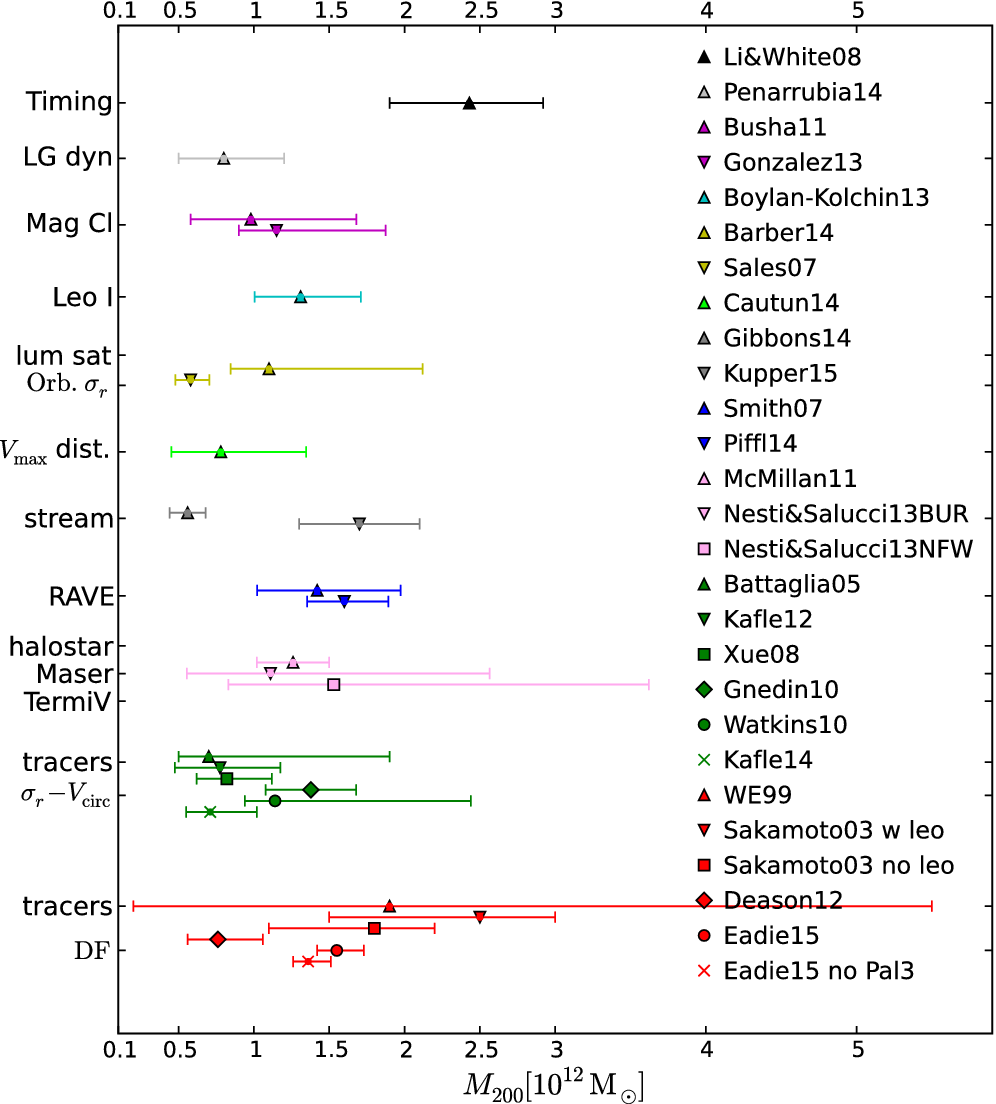
\includegraphics[width=0.7\textwidth]{kuvat/wang2015-masses.png}
   \caption{$M_{200}$ masses of the Milky Way as obtained by different authors using various mass estimation methods, collected and plotted by \citet{wang2015estimating}. Error bars show the $1\sigma$ range where assuming Gaussian distribution was appropriate. Masses derived using similar methods are plotted in same colour.}
   \label{fig:wang-masses}
\end{figure}

Different papers present varying values for the masses of the Local Group and its galaxies, both due to the strengths and limitations of the methods used and differences in the used observed and simulated data. A collection of mass estimates for Milky Way is shown in figure \ref{fig:wang-masses} by \citet{wang2015estimating}. The masses are calculated by different authors using various mass estimation methods, some of which have been briefly introduced in this section. The plot clearly illustrates the fact that currently the masses of the Local Group galaxies have errors of over a factor of two.

Especially the timing argument stands out from the other methods. This is in agreement with a study of \citet{gonzalez2014mass} where timing argument masses were found to overestimate the true mass of a Local Group like system with small tangential velocity and low local overdensity by a mean factor of 1.6. This is due to the timing argument not being sensitive to the tangential velocity or environment of the system.

The other mass estimates also have considerable scatter, sometimes even within the same mass estimation method. At least some of this scatter can be a result of some estimates being more than ten years old and thus their methods and data possibly outdated, but the scatter also reflects the fact that the exact mass of the Local Group is currently a question without a definitive answer. Thus exploring new ways of estimating the mass and refining the old results is important.



\chapter{Simulations and Simulation Codes}

Numerical simulations are a valuable tool in astrophysical research as they bypass many major restrictions characteristic to observational astronomy. For example the dark matter content of the Universe cannot be directly observed and following the evolution of a single object is impossible, with the exception of the most rapid events such as supernovae. Much can also be done using analytical models, but they are often valid only for a simplified problem or suffer from other limitations. For example the Zel'dovich approximation can be used to calculate the non-linear evolution of density perturbations in the Universe up to shell crossing, but after the structures have collapsed to sheets along one of their axes, the model ceases to be valid \citep{mo2010galaxy}.

The data used in this master's thesis also originates from a cosmological N\=/body simulation. This section shortly introduces first some fundamental operational principles of N\=/body simulations and then discusses specifics of the simulations from which the data used here originates from. Lastly, the extraction and properties of the resulting data set are discussed.


\section{N\=/Body Simulations}
N\=/body simulations are a type of computer simulations that follow a number of particles interacting with each other \citep{binney2008galactic}. They are often used in computational astrophysics as well as other fields of physics. For some applications, including for example simulating motions of planets in a planetary system, it is possible to have each body represented by a single simulation particle. This kind of simulations are run using collisional N\=/body codes \citep{binney2008galactic}. In cosmological simulations the number of simulated objects such as stars let alone dark matter particles is too great for them to be simulated as separate particles. In this case a collisionless N\=/body simulation is used, meaning that the simulated volume is approximated to contain a smooth density field, evolution of which is studied by following a number of particles representing the system \citep{binney2008galactic}. These particles do not correspond to any real structures but instead they can be thought to sample the probability density distribution (see section \ref{sect:distribution-functions} for more on probability distributions) of positions and velocities \citep{binney2008galactic}. In this thesis, only collisionless simulations are discussed.

The concept of both collisional and collisionless N\=/body simulations is simple: the current positions and velocities of the particles are known and a physical model is used to calculate how they should advance over a small period of time known as the time step \citep{binney2008galactic}. Simple dark matter only simulations might only handle gravitational interactions of the particles, but many simulation codes such as \textsc{gadget-3} \citep{springel2005cosmological} (see section \ref{sect:gadget} for more about \textsc{gadget} family simulation codes) and Enzo \citep{norman2007simulating} are also able to simulate hydrodynamics of baryonic matter and can include star formation, feedback and other baryonic processes.

As the particles of a collisionless system are not any real structures, e.g. stars, star clusters or galaxies, the situation in which two particles come near each other and thus feel strong forces resulting in large accelerations is problematic \citep{binney2008galactic}. This is because the underlying density distribution is smooth and thus such two-body scattering is unphysical. The problem can be alleviated by softening, i.e. modifying the gravitational force calculations so that for small interparticle distances the force diminishes \citep{binney2008galactic}. At large separations the force remains unchanged, and the distance within which the force differs from Newtonian gravity is called the softening length \citep{binney2008galactic}.

There are multiple ways to handle both the force calculations and updating the positions and velocities for the particles \citep{binney2008galactic}. For the force calculations, the most popular algorithms are based on either hierarchical trees or particle meshes, but for updating the positions, a wide variety of integrators have been developed for a range of different needs \citep{binney2008galactic}. The simulations discussed in this thesis are run using a modified version of \textsc{gadget-3} and thus use the TreePM method for force calculations accompanied by a leapfrog integrator. TreePM is a mix of a hierarchical tree for short-range forces and a particle mesh for long-range forces. The description of the particle mesh is omitted, but the \citet{barnes1986hierarchical} hierarchical tree algorithm is introduced in the following subsection, followed by a short description of the leapfrog integrator.

\subsection{Hierarchical Tree Algorithm} \label{sect:tree}
In many applications of computational astrophysics the desired number of particles in a simulation is too great to allow calculating interparticle forces by direct summation as its time complexity is $\mathcal{O}(n^2)$, where $n$ is the number of particles in the simulation. One of the alternatives is to organize the particles into a tree data structure, which allows distant particles residing close to each other to be approximated as a single more massive particle. This approach was first introduced by \citet{appel1985efficient} and \citet{barnes1986hierarchical}, the latter of which will be followed here.

Constructing the tree starts with setting the full simulation box as the root of the tree. This root cube is then subdivided into eight equally sized sub-cubes called cells. These eight cells are children of the root node. This starts a recursive process where each new cell is again divided into eight subcells recursively until each of the cells contains either no particles, one particle or eight subcells. When a new cell is created, the total mass of the enclosed particles and the location of the mass centre of the particles within it is stored as a pseudoparticle to allow easy calculation of the approximate gravitational effect the particles within a cell have on a distant particle.

\begin{figure}
    \centering
    %\def\svgwidth{\columnwidth}
    \input{kuvat/tex/tree-box.pdf_tex}
    \caption{A two-dimensional example of particles (black dots) being assigned to cells using the Barnes-Hut algorithm \citep{barnes1986hierarchical}. The outermost square is the simulation box, i.e. the root of the tree, and the smaller squares with decreasing line thicknesses are its descendants. Note how each cell contains either one particle, no particles or four smaller subcells, each of which may be further divided into subcells of their own.}\label{fig:tree-box}
\end{figure}

\begin{figure}
    \centering
    \def\svgwidth{\columnwidth}
    \input{kuvat/tex/tree-solids.pdf_tex}
    \caption{Cells of Fig.\ \ref{fig:tree-box} shown as a tree, each level of subcells in Fig.\ \ref{fig:tree-box} traversed from left to right and top to bottom corresponding to each level of nodes from left to right. Cells containing one or more particles are shown as filled circles. Cells with no particles are not used in force calculations and thus they do not need to be stored in computer memory, but they are shown here as non-filled circles to emphasize the structure of the tree.}\label{fig:tree}
\end{figure}

To aid in understanding the process, a two-dimensional simplification of the simulation box divided into cells is shown in Fig.\ \ref{fig:tree-box}, together with the corresponding tree in Fig.\ \ref{fig:tree}. The thick outer line of Fig.\ \ref{fig:tree-box} is the simulation box, corresponding to the topmost node of the tree in Fig.\ \ref{fig:tree}. This root cell is first divided into four subcells (in contrast to the eight subcells in the three-dimensional case), which is shown with the second-thickest line dividing the simulation box into quarters in Fig.\ \ref{fig:tree-box}. These four cells are the four children of the root node in the tree. Each of the subcells contains more than one particle, so each subcell is again split into four quarters, each of them thus receiving four new child nodes. The newly-created quarters of quarters form the third level of the tree in Fig.\ \ref{fig:tree}.

Some of these new cells are empty or only have a single particle. For them the recursion halts and the nodes of the tree are leaves. The rest are again split and a new level is added to the tree, but as some cells were complete already the fourth level of the tree is not full. In this particular case only one cell requires division beyond the fourth level, producing the last four leaves of the tree on the fifth level.

Often, as is the case in this example, some of the leaf nodes contain no particles. In the case of a real simulation, these cells of course do not need to be saved as there is no information to store, but in this example case all are drawn to emphasize the regular structure of the tree. In the three-dimensional case, where each internal cell has eight subcells, the formed tree is known as an octree, whose two-dimensional analogue, the quadtree, is constructed in the previous example.

After constructing the tree, it can be utilized to speed up the force calculations. When calculating the gravitational acceleration felt by a single particle, the tree is traversed starting from the root. The ratio $l/D$ of the length of a side of the cell ($l$) and the distance from the particle to the pseudoparticle representing the centre of mass within the cell ($D$) is then calculated. If the ratio is smaller than a predefined accuracy parameter $\theta$ representing the opening angle of the cell, the cell is treated as if everything within it was replaced with the pseudoparticle having the combined mass of the cell. Otherwise the subcells of the cell are examined recursively in the same way until a small enough subcell is found or a leaf of the tree is reached, at which point the pseudoparticle and the real particle in the cell are equivalent and the force can be calculated with the maximum accuracy possible for the simulation.

Using the Barnes-Hut algorithm, the tree construction and the force calculations both have time complexity of $\mathcal{O}(n \log n)$. This is a significant improvement over the $\mathcal{O}(n^2)$ of the direct summation considering that the accuracy cost is fairly small: \citet{barnes1986hierarchical} report accuracy of about 1~\% for a single force evaluation when $\theta=1$ and the accuracy can be improved by either setting a smaller $\theta$ or including multipole moments in the pseudoparticles \citep{barnes1989error}. %Similar algorithms with even better time complexity of $\mathcal{O}(n)$ have also been introduced such as those by \citet{dehnen2002hierarchical} and \citet{xue1998n}.

The algorithm is also straightforward to parallelize as different branches of the tree can be assigned to their own threads, though memory management has to be done carefully when forces outside the current branch of a thread are calculated \citep{binney2008galactic}. One way to circumvent the memory management issue is to use a particle mesh based integrator for long range forces as \textsc{gadget-3} does \citep{springel2005cosmological}. The algorithm can also handle problems where the range of densities in the simulation box is large, which is important for applications such as galaxy mergers and cosmological simulations. This, together with their competitive time complexity, makes tree based codes an appealing tool for many astrophysical simulations \citep{binney2008galactic}.


\subsection{Leapfrog Integrator} \label{sect:leapfrog}
A number of different integrators suitable for astronomical and astrophysical applications have been developed  for solving different problems \citep{binney2008galactic}. No integrator is optimal for every task and thus factors such as the integration time, amount of memory available per particle, smoothness of the potential and the cost of a single gravitational field evaluation should be considered \citep{binney2008galactic}. One of the integrators that are well suited for cosmological simulations is the leapfrog integrator, which is also used by \textsc{gadget-3} simulation code \citep{springel2005cosmological}.

When a fixed time step is used, the leapfrog integrator conserves the energy of the system and is time-reversible \citep{binney2008galactic}. While a variable time step is possible and often used, it requires some modifications to the algorithm, presented in e.g. \citet{springel2005cosmological} and implemented in the \textsc{gadget-3} simulation code among others. Other benefits of the integrator are its second order accuracy and the fact that it does not require excessive amounts of memory per particle as only the current state of the system is needed in calculating the next step \citep{binney2008galactic}. It is also second-order accurate and symplectic \citep{binney2008galactic}. Due to symplecticity of the integrator, numerical dissipation of energy does not happen and thus the integrator rivals some integrators with higher-order accuracy such as the fourth order Runge-Kutta when the number of simulated time steps is large \citep{binney2008galactic}.

%With its second order accuracy paired with symplecticity, numerical dissipation of energy does not happen and thus it rivals some integrators with higher-order accuracy such as the fourth order Runge-Kutta when used for long simulation runs \citep{binney2008galactic}.


% won't work for an unknown reason
%\begin{figure}
%    \centering
%    %\def\svgwidth{\columnwidth}
%    \input{kuvat/tex/leapfrog.pdf_tex}
%    \caption{adsf}\label{fig:leapfrog}
%\end{figure}

\begin{figure}
\centering
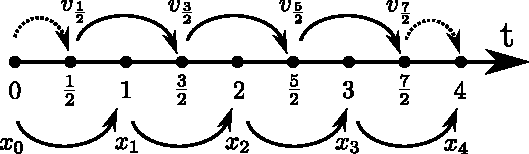
\includegraphics{kuvat/tex/leapfrog.pdf}
\caption{Timesteps taken by the leapfrog algorithm, with positions ($x$) updated as indicated with the lower arrows and velocities ($v$) as indicated by the upper arrows. It is not important for the algorithm which of the two is chosen to step through the integer times, the choice of it being $x$ in this figure is arbitrary. The dashed short arrows depict the half-steps that are needed when a synchronized output is desired.}\label{fig:leapfrog}
\end{figure}

Timestepping with the leapfrog integrator consists of two phases, the drift and the kick steps, which are alternated with a half-step offset as shown in Fig.\ \ref{fig:leapfrog} \citep{binney2008galactic}. During the kick step, the momenta of the particles are updated and during the drift step the positions of the particles are changed according to the momenta calculated during the kick step \citep{binney2008galactic}. When synchronized output of both positions and velocities is desired, a half-timestep advance or backtrack to one of the variables is needed to determine their values at the same point in time. This kind of synchronization steps at start and end of the integration are indicated in Fig.\ \ref{fig:leapfrog} with dashed arrows.


\subsection{Halo Finding} \label{sect:halofinding}
The data output by a cosmological simulation consists of individual particles tracing the underlying density field. To make comparisons with the real Universe, a way of matching structures in the simulation to observable objects is needed. In a dark matter only simulation no structure would obviously be directly observable but luckily many properties of dark matter haloes from simulations can be compared with the estimated dark matter haloes of observed galaxies. Making such comparisons naturally requires structures to be identified first, which makes structure finding a key step in the data analysis for many astrophysical and cosmological applications \citep{knebe2013structure}.

A number of different halo finders designed to read N\=/body data and extract locally overdense gravitationally bound systems have been developed to suit different needs, most based either on locating density peaks or collecting and linking together particles located close to each other based on some metric \citep{knebe2013structure}. Two methods, the friends-of-friends (\textsc{fof}) and \textsc{subfind} algorithms, are discussed here. Both algorithms were developed separately, \textsc{fof} by \citet{davis1985evolution} and \textsc{subfind} by \citet{springel2001populating}, but they work well when used together by inputting \textsc{fof} results to \textsc{subfind} as a starting point for the subhalo finding \citep{springel2005cosmological}.

The \textsc{fof} algorithm is simple and based purely on the spatial separation of the particles: pairs of particles residing closer to each other than a chosen threshold distance called the linking length are marked to reside within the same group by linking them together \citep{davis1985evolution}. When all particles have been processed, each distinct subset of particles linked to each other is defined to be a group \citep{davis1985evolution}. Figure \ref{fig:fof} presents an example of a set of particles grouped using the \textsc{fof} algorithm. Depending on the specifics of the data and its intended usage, one might want to discard the smallest groups with only a few particles. This is because they are more likely than bigger groups to be just realizations of the random noise instead of actual physical structures, but also as they might not be massive enough to represent the structures that are being studied.

\begin{figure}
    \centering
    %\def\svgwidth{\columnwidth}
    %LaTeX with PSTricks extensions
%%Creator: inkscape 0.91
%%Please note this file requires PSTricks extensions
\psset{xunit=.5pt,yunit=.5pt,runit=.5pt}
\begin{pspicture}(336.84284781,197.28769017)
{
\newrgbcolor{curcolor}{0 0 0}
\pscustom[linewidth=2.19999985,linecolor=curcolor]
{
\newpath
\moveto(233.19734446,178.3399713)
\lineto(259.35586134,178.13219131)
}
}
{
\newrgbcolor{curcolor}{0 0 0}
\pscustom[linewidth=1.09999993,linecolor=curcolor]
{
\newpath
\moveto(233.15785257,173.36812833)
\lineto(233.23683635,183.31181427)
}
}
{
\newrgbcolor{curcolor}{0 0 0}
\pscustom[linewidth=1.09999993,linecolor=curcolor]
{
\newpath
\moveto(259.31636945,173.16034834)
\lineto(259.39535323,183.10403428)
}
}
{
\newrgbcolor{curcolor}{0 0 0}
\pscustom[linestyle=none,fillstyle=solid,fillcolor=curcolor]
{
\newpath
\moveto(203.78160797,197.28768017)
\lineto(201.63660822,197.12268018)
\lineto(201.63660822,196.65768021)
\curveto(202.6866081,196.65768021)(202.80660808,196.55268021)(202.80660808,195.81768026)
\lineto(202.80660808,188.04768072)
\curveto(202.80660808,187.37268076)(202.6416081,187.37268076)(201.63660822,187.37268076)
\lineto(201.63660822,186.90768079)
\curveto(202.13160816,186.92268079)(202.92660807,186.95268079)(203.30160802,186.95268079)
\curveto(203.66160798,186.95268079)(204.39660789,186.92268079)(204.95160783,186.90768079)
\lineto(204.95160783,187.37268076)
\curveto(203.94660795,187.37268076)(203.78160797,187.37268076)(203.78160797,188.04768072)
\closepath
}
}
{
\newrgbcolor{curcolor}{0 0 0}
\pscustom[linewidth=0,linecolor=curcolor]
{
\newpath
\moveto(203.78160797,197.28768017)
\lineto(201.63660822,197.12268018)
\lineto(201.63660822,196.65768021)
\curveto(202.6866081,196.65768021)(202.80660808,196.55268021)(202.80660808,195.81768026)
\lineto(202.80660808,188.04768072)
\curveto(202.80660808,187.37268076)(202.6416081,187.37268076)(201.63660822,187.37268076)
\lineto(201.63660822,186.90768079)
\curveto(202.13160816,186.92268079)(202.92660807,186.95268079)(203.30160802,186.95268079)
\curveto(203.66160798,186.95268079)(204.39660789,186.92268079)(204.95160783,186.90768079)
\lineto(204.95160783,187.37268076)
\curveto(203.94660795,187.37268076)(203.78160797,187.37268076)(203.78160797,188.04768072)
\closepath
}
}
{
\newrgbcolor{curcolor}{0 0 0}
\pscustom[linestyle=none,fillstyle=solid,fillcolor=curcolor]
{
\newpath
\moveto(207.93660747,193.52268039)
\lineto(205.85160772,193.3576804)
\lineto(205.85160772,192.89268043)
\curveto(206.8116076,192.89268043)(206.94660759,192.80268044)(206.94660759,192.06768048)
\lineto(206.94660759,188.04768072)
\curveto(206.94660759,187.37268076)(206.78160761,187.37268076)(205.79160773,187.37268076)
\lineto(205.79160773,186.90768079)
\curveto(206.25660767,186.92268079)(207.06660757,186.95268079)(207.42660753,186.95268079)
\curveto(207.95160747,186.95268079)(208.47660741,186.92268079)(208.98660735,186.90768079)
\lineto(208.98660735,187.37268076)
\curveto(207.99660746,187.37268076)(207.93660747,187.44768076)(207.93660747,188.03268072)
\closepath
}
}
{
\newrgbcolor{curcolor}{0 0 0}
\pscustom[linewidth=0,linecolor=curcolor]
{
\newpath
\moveto(207.93660747,193.52268039)
\lineto(205.85160772,193.3576804)
\lineto(205.85160772,192.89268043)
\curveto(206.8116076,192.89268043)(206.94660759,192.80268044)(206.94660759,192.06768048)
\lineto(206.94660759,188.04768072)
\curveto(206.94660759,187.37268076)(206.78160761,187.37268076)(205.79160773,187.37268076)
\lineto(205.79160773,186.90768079)
\curveto(206.25660767,186.92268079)(207.06660757,186.95268079)(207.42660753,186.95268079)
\curveto(207.95160747,186.95268079)(208.47660741,186.92268079)(208.98660735,186.90768079)
\lineto(208.98660735,187.37268076)
\curveto(207.99660746,187.37268076)(207.93660747,187.44768076)(207.93660747,188.03268072)
\closepath
}
}
{
\newrgbcolor{curcolor}{0 0 0}
\pscustom[linestyle=none,fillstyle=solid,fillcolor=curcolor]
{
\newpath
\moveto(207.99660746,196.11768024)
\lineto(207.99660746,196.16268024)
\lineto(207.99660746,196.20768023)
\lineto(207.98160747,196.25268023)
\lineto(207.98160747,196.28268023)
\lineto(207.96660747,196.32768023)
\lineto(207.96660747,196.37268022)
\lineto(207.95160747,196.40268022)
\lineto(207.93660747,196.44768022)
\lineto(207.92160747,196.47768022)
\lineto(207.89160748,196.50768022)
\lineto(207.87660748,196.53768021)
\lineto(207.86160748,196.58268021)
\lineto(207.83160748,196.61268021)
\lineto(207.81660749,196.64268021)
\lineto(207.78660749,196.65768021)
\lineto(207.75660749,196.68768021)
\lineto(207.7266075,196.7176802)
\lineto(207.6966075,196.7476802)
\lineto(207.6666075,196.7626802)
\lineto(207.63660751,196.7776802)
\lineto(207.60660751,196.8076802)
\lineto(207.57660751,196.8226802)
\lineto(207.54660752,196.8376802)
\lineto(207.50160752,196.8526802)
\lineto(207.47160753,196.8676802)
\lineto(207.44160753,196.88268019)
\lineto(207.39660754,196.88268019)
\lineto(207.36660754,196.89768019)
\lineto(207.32160754,196.89768019)
\lineto(207.27660755,196.89768019)
\lineto(207.24660755,196.91268019)
\lineto(207.20160756,196.91268019)
\curveto(206.73660761,196.91268019)(206.42160765,196.50768022)(206.42160765,196.11768024)
\curveto(206.42160765,195.71268026)(206.73660761,195.32268029)(207.20160756,195.32268029)
\curveto(207.62160751,195.32268029)(207.99660746,195.63768027)(207.99660746,196.11768024)
\closepath
}
}
{
\newrgbcolor{curcolor}{0 0 0}
\pscustom[linewidth=0,linecolor=curcolor]
{
\newpath
\moveto(207.99660746,196.11768024)
\lineto(207.99660746,196.16268024)
\lineto(207.99660746,196.20768023)
\lineto(207.98160747,196.25268023)
\lineto(207.98160747,196.28268023)
\lineto(207.96660747,196.32768023)
\lineto(207.96660747,196.37268022)
\lineto(207.95160747,196.40268022)
\lineto(207.93660747,196.44768022)
\lineto(207.92160747,196.47768022)
\lineto(207.89160748,196.50768022)
\lineto(207.87660748,196.53768021)
\lineto(207.86160748,196.58268021)
\lineto(207.83160748,196.61268021)
\lineto(207.81660749,196.64268021)
\lineto(207.78660749,196.65768021)
\lineto(207.75660749,196.68768021)
\lineto(207.7266075,196.7176802)
\lineto(207.6966075,196.7476802)
\lineto(207.6666075,196.7626802)
\lineto(207.63660751,196.7776802)
\lineto(207.60660751,196.8076802)
\lineto(207.57660751,196.8226802)
\lineto(207.54660752,196.8376802)
\lineto(207.50160752,196.8526802)
\lineto(207.47160753,196.8676802)
\lineto(207.44160753,196.88268019)
\lineto(207.39660754,196.88268019)
\lineto(207.36660754,196.89768019)
\lineto(207.32160754,196.89768019)
\lineto(207.27660755,196.89768019)
\lineto(207.24660755,196.91268019)
\lineto(207.20160756,196.91268019)
\curveto(206.73660761,196.91268019)(206.42160765,196.50768022)(206.42160765,196.11768024)
\curveto(206.42160765,195.71268026)(206.73660761,195.32268029)(207.20160756,195.32268029)
\curveto(207.62160751,195.32268029)(207.99660746,195.63768027)(207.99660746,196.11768024)
\closepath
}
}
{
\newrgbcolor{curcolor}{0 0 0}
\pscustom[linestyle=none,fillstyle=solid,fillcolor=curcolor]
{
\newpath
\moveto(211.0866071,192.05268048)
\lineto(211.0866071,188.04768072)
\curveto(211.0866071,187.37268076)(210.92160711,187.37268076)(209.91660723,187.37268076)
\lineto(209.91660723,186.90768079)
\curveto(210.44160717,186.92268079)(211.20660708,186.95268079)(211.61160703,186.95268079)
\curveto(212.00160699,186.95268079)(212.78160689,186.92268079)(213.27660683,186.90768079)
\lineto(213.27660683,187.37268076)
\curveto(212.28660695,187.37268076)(212.12160697,187.37268076)(212.12160697,188.04768072)
\lineto(212.12160697,190.79268056)
\curveto(212.12160697,192.35268046)(213.18660684,193.19268041)(214.13160673,193.19268041)
\curveto(215.07660662,193.19268041)(215.2416066,192.38268046)(215.2416066,191.52768051)
\lineto(215.2416066,188.04768072)
\curveto(215.2416066,187.37268076)(215.07660662,187.37268076)(214.07160674,187.37268076)
\lineto(214.07160674,186.90768079)
\curveto(214.59660668,186.92268079)(215.36160659,186.95268079)(215.76660654,186.95268079)
\curveto(216.15660649,186.95268079)(216.9366064,186.92268079)(217.43160634,186.90768079)
\lineto(217.43160634,187.37268076)
\curveto(216.66660643,187.37268076)(216.29160647,187.37268076)(216.27660648,187.82268073)
\lineto(216.27660648,190.67268056)
\curveto(216.27660648,191.96268049)(216.27660648,192.42768046)(215.81160653,192.96768043)
\curveto(215.60160656,193.22268041)(215.10660662,193.52268039)(214.23660672,193.52268039)
\curveto(213.15660685,193.52268039)(212.45160693,192.87768043)(212.03160698,191.94768049)
\lineto(212.03160698,193.52268039)
\lineto(209.91660723,193.3576804)
\lineto(209.91660723,192.89268043)
\curveto(210.96660711,192.89268043)(211.0866071,192.78768044)(211.0866071,192.05268048)
\closepath
}
}
{
\newrgbcolor{curcolor}{0 0 0}
\pscustom[linewidth=0,linecolor=curcolor]
{
\newpath
\moveto(211.0866071,192.05268048)
\lineto(211.0866071,188.04768072)
\curveto(211.0866071,187.37268076)(210.92160711,187.37268076)(209.91660723,187.37268076)
\lineto(209.91660723,186.90768079)
\curveto(210.44160717,186.92268079)(211.20660708,186.95268079)(211.61160703,186.95268079)
\curveto(212.00160699,186.95268079)(212.78160689,186.92268079)(213.27660683,186.90768079)
\lineto(213.27660683,187.37268076)
\curveto(212.28660695,187.37268076)(212.12160697,187.37268076)(212.12160697,188.04768072)
\lineto(212.12160697,190.79268056)
\curveto(212.12160697,192.35268046)(213.18660684,193.19268041)(214.13160673,193.19268041)
\curveto(215.07660662,193.19268041)(215.2416066,192.38268046)(215.2416066,191.52768051)
\lineto(215.2416066,188.04768072)
\curveto(215.2416066,187.37268076)(215.07660662,187.37268076)(214.07160674,187.37268076)
\lineto(214.07160674,186.90768079)
\curveto(214.59660668,186.92268079)(215.36160659,186.95268079)(215.76660654,186.95268079)
\curveto(216.15660649,186.95268079)(216.9366064,186.92268079)(217.43160634,186.90768079)
\lineto(217.43160634,187.37268076)
\curveto(216.66660643,187.37268076)(216.29160647,187.37268076)(216.27660648,187.82268073)
\lineto(216.27660648,190.67268056)
\curveto(216.27660648,191.96268049)(216.27660648,192.42768046)(215.81160653,192.96768043)
\curveto(215.60160656,193.22268041)(215.10660662,193.52268039)(214.23660672,193.52268039)
\curveto(213.15660685,193.52268039)(212.45160693,192.87768043)(212.03160698,191.94768049)
\lineto(212.03160698,193.52268039)
\lineto(209.91660723,193.3576804)
\lineto(209.91660723,192.89268043)
\curveto(210.96660711,192.89268043)(211.0866071,192.78768044)(211.0866071,192.05268048)
\closepath
}
}
{
\newrgbcolor{curcolor}{0 0 0}
\pscustom[linestyle=none,fillstyle=solid,fillcolor=curcolor]
{
\newpath
\moveto(219.33660611,188.04768072)
\lineto(219.33660611,188.01768072)
\lineto(219.33660611,187.98768072)
\lineto(219.32160611,187.92768073)
\lineto(219.32160611,187.88268073)
\lineto(219.32160611,187.82268073)
\lineto(219.32160611,187.77768074)
\lineto(219.30660612,187.73268074)
\lineto(219.30660612,187.70268074)
\lineto(219.29160612,187.65768074)
\lineto(219.27660612,187.62768075)
\lineto(219.26160612,187.59768075)
\lineto(219.24660612,187.56768075)
\lineto(219.23160612,187.53768075)
\lineto(219.20160613,187.52268075)
\lineto(219.18660613,187.49268075)
\lineto(219.15660613,187.47768075)
\lineto(219.12660614,187.46268076)
\lineto(219.09660614,187.44768076)
\lineto(219.05160615,187.43268076)
\lineto(219.02160615,187.41768076)
\lineto(218.97660615,187.40268076)
\lineto(218.93160616,187.40268076)
\lineto(218.87160617,187.38768076)
\lineto(218.82660617,187.38768076)
\lineto(218.76660618,187.38768076)
\lineto(218.73660618,187.38768076)
\lineto(218.70660619,187.38768076)
\lineto(218.67660619,187.37268076)
\lineto(218.64660619,187.37268076)
\lineto(218.6166062,187.37268076)
\lineto(218.5716062,187.37268076)
\lineto(218.54160621,187.37268076)
\lineto(218.49660621,187.37268076)
\lineto(218.46660622,187.37268076)
\lineto(218.42160622,187.37268076)
\lineto(218.39160622,187.37268076)
\lineto(218.34660623,187.37268076)
\lineto(218.30160624,187.37268076)
\lineto(218.25660624,187.37268076)
\lineto(218.21160625,187.37268076)
\lineto(218.16660625,187.37268076)
\lineto(218.16660625,186.90768079)
\curveto(218.66160619,186.92268079)(219.36660611,186.95268079)(219.80160606,186.95268079)
\curveto(220.236606,186.95268079)(220.83660593,186.93768079)(221.43660586,186.90768079)
\lineto(221.43660586,187.37268076)
\curveto(220.43160598,187.37268076)(220.266606,187.37268076)(220.266606,188.04768072)
\lineto(220.266606,189.59268063)
\lineto(221.22660589,190.40268058)
\curveto(222.38160575,188.82768067)(223.01160567,187.98768072)(223.01160567,187.71768074)
\curveto(223.01160567,187.43268076)(222.7566057,187.37268076)(222.47160574,187.37268076)
\lineto(222.47160574,186.90768079)
\curveto(222.89160569,186.92268079)(223.76160558,186.95268079)(224.07660555,186.95268079)
\curveto(224.51160549,186.95268079)(224.94660544,186.93768079)(225.38160539,186.90768079)
\lineto(225.38160539,187.37268076)
\curveto(224.82660546,187.37268076)(224.4966055,187.37268076)(223.92660556,188.16768071)
\lineto(222.03660579,190.83768055)
\curveto(222.02160579,190.86768055)(221.9466058,190.95768055)(221.9466058,191.00268054)
\curveto(221.9466058,191.06268054)(223.01160567,191.96268049)(223.16160566,192.08268048)
\curveto(224.09160554,192.84768043)(224.72160547,192.87768043)(225.03660543,192.89268043)
\lineto(225.03660543,193.3576804)
\curveto(224.60160548,193.31268041)(224.40660551,193.31268041)(223.98660556,193.31268041)
\curveto(223.46160562,193.31268041)(222.53160573,193.34268041)(222.32160576,193.3576804)
\lineto(222.32160576,192.89268043)
\curveto(222.60660572,192.87768043)(222.7566057,192.71268044)(222.7566057,192.51768045)
\curveto(222.7566057,192.21768047)(222.54660573,192.03768048)(222.42660574,191.93268049)
\lineto(220.311606,190.1176806)
\lineto(220.311606,197.28768017)
\lineto(218.16660625,197.12268018)
\lineto(218.16660625,196.65768021)
\curveto(219.21660613,196.65768021)(219.33660611,196.55268021)(219.33660611,195.81768026)
\closepath
}
}
{
\newrgbcolor{curcolor}{0 0 0}
\pscustom[linewidth=0,linecolor=curcolor]
{
\newpath
\moveto(219.33660611,188.04768072)
\lineto(219.33660611,188.01768072)
\lineto(219.33660611,187.98768072)
\lineto(219.32160611,187.92768073)
\lineto(219.32160611,187.88268073)
\lineto(219.32160611,187.82268073)
\lineto(219.32160611,187.77768074)
\lineto(219.30660612,187.73268074)
\lineto(219.30660612,187.70268074)
\lineto(219.29160612,187.65768074)
\lineto(219.27660612,187.62768075)
\lineto(219.26160612,187.59768075)
\lineto(219.24660612,187.56768075)
\lineto(219.23160612,187.53768075)
\lineto(219.20160613,187.52268075)
\lineto(219.18660613,187.49268075)
\lineto(219.15660613,187.47768075)
\lineto(219.12660614,187.46268076)
\lineto(219.09660614,187.44768076)
\lineto(219.05160615,187.43268076)
\lineto(219.02160615,187.41768076)
\lineto(218.97660615,187.40268076)
\lineto(218.93160616,187.40268076)
\lineto(218.87160617,187.38768076)
\lineto(218.82660617,187.38768076)
\lineto(218.76660618,187.38768076)
\lineto(218.73660618,187.38768076)
\lineto(218.70660619,187.38768076)
\lineto(218.67660619,187.37268076)
\lineto(218.64660619,187.37268076)
\lineto(218.6166062,187.37268076)
\lineto(218.5716062,187.37268076)
\lineto(218.54160621,187.37268076)
\lineto(218.49660621,187.37268076)
\lineto(218.46660622,187.37268076)
\lineto(218.42160622,187.37268076)
\lineto(218.39160622,187.37268076)
\lineto(218.34660623,187.37268076)
\lineto(218.30160624,187.37268076)
\lineto(218.25660624,187.37268076)
\lineto(218.21160625,187.37268076)
\lineto(218.16660625,187.37268076)
\lineto(218.16660625,186.90768079)
\curveto(218.66160619,186.92268079)(219.36660611,186.95268079)(219.80160606,186.95268079)
\curveto(220.236606,186.95268079)(220.83660593,186.93768079)(221.43660586,186.90768079)
\lineto(221.43660586,187.37268076)
\curveto(220.43160598,187.37268076)(220.266606,187.37268076)(220.266606,188.04768072)
\lineto(220.266606,189.59268063)
\lineto(221.22660589,190.40268058)
\curveto(222.38160575,188.82768067)(223.01160567,187.98768072)(223.01160567,187.71768074)
\curveto(223.01160567,187.43268076)(222.7566057,187.37268076)(222.47160574,187.37268076)
\lineto(222.47160574,186.90768079)
\curveto(222.89160569,186.92268079)(223.76160558,186.95268079)(224.07660555,186.95268079)
\curveto(224.51160549,186.95268079)(224.94660544,186.93768079)(225.38160539,186.90768079)
\lineto(225.38160539,187.37268076)
\curveto(224.82660546,187.37268076)(224.4966055,187.37268076)(223.92660556,188.16768071)
\lineto(222.03660579,190.83768055)
\curveto(222.02160579,190.86768055)(221.9466058,190.95768055)(221.9466058,191.00268054)
\curveto(221.9466058,191.06268054)(223.01160567,191.96268049)(223.16160566,192.08268048)
\curveto(224.09160554,192.84768043)(224.72160547,192.87768043)(225.03660543,192.89268043)
\lineto(225.03660543,193.3576804)
\curveto(224.60160548,193.31268041)(224.40660551,193.31268041)(223.98660556,193.31268041)
\curveto(223.46160562,193.31268041)(222.53160573,193.34268041)(222.32160576,193.3576804)
\lineto(222.32160576,192.89268043)
\curveto(222.60660572,192.87768043)(222.7566057,192.71268044)(222.7566057,192.51768045)
\curveto(222.7566057,192.21768047)(222.54660573,192.03768048)(222.42660574,191.93268049)
\lineto(220.311606,190.1176806)
\lineto(220.311606,197.28768017)
\lineto(218.16660625,197.12268018)
\lineto(218.16660625,196.65768021)
\curveto(219.21660613,196.65768021)(219.33660611,196.55268021)(219.33660611,195.81768026)
\closepath
}
}
{
\newrgbcolor{curcolor}{0 0 0}
\pscustom[linestyle=none,fillstyle=solid,fillcolor=curcolor]
{
\newpath
\moveto(228.27660505,193.52268039)
\lineto(226.19160529,193.3576804)
\lineto(226.19160529,192.89268043)
\curveto(227.15160518,192.89268043)(227.28660516,192.80268044)(227.28660516,192.06768048)
\lineto(227.28660516,188.04768072)
\curveto(227.28660516,187.37268076)(227.12160518,187.37268076)(226.1316053,187.37268076)
\lineto(226.1316053,186.90768079)
\curveto(226.59660525,186.92268079)(227.40660515,186.95268079)(227.76660511,186.95268079)
\curveto(228.29160504,186.95268079)(228.81660498,186.92268079)(229.32660492,186.90768079)
\lineto(229.32660492,187.37268076)
\curveto(228.33660504,187.37268076)(228.27660505,187.44768076)(228.27660505,188.03268072)
\closepath
}
}
{
\newrgbcolor{curcolor}{0 0 0}
\pscustom[linewidth=0,linecolor=curcolor]
{
\newpath
\moveto(228.27660505,193.52268039)
\lineto(226.19160529,193.3576804)
\lineto(226.19160529,192.89268043)
\curveto(227.15160518,192.89268043)(227.28660516,192.80268044)(227.28660516,192.06768048)
\lineto(227.28660516,188.04768072)
\curveto(227.28660516,187.37268076)(227.12160518,187.37268076)(226.1316053,187.37268076)
\lineto(226.1316053,186.90768079)
\curveto(226.59660525,186.92268079)(227.40660515,186.95268079)(227.76660511,186.95268079)
\curveto(228.29160504,186.95268079)(228.81660498,186.92268079)(229.32660492,186.90768079)
\lineto(229.32660492,187.37268076)
\curveto(228.33660504,187.37268076)(228.27660505,187.44768076)(228.27660505,188.03268072)
\closepath
}
}
{
\newrgbcolor{curcolor}{0 0 0}
\pscustom[linestyle=none,fillstyle=solid,fillcolor=curcolor]
{
\newpath
\moveto(228.33660504,196.11768024)
\lineto(228.33660504,196.16268024)
\lineto(228.33660504,196.20768023)
\lineto(228.32160504,196.25268023)
\lineto(228.32160504,196.28268023)
\lineto(228.30660504,196.32768023)
\lineto(228.30660504,196.37268022)
\lineto(228.29160504,196.40268022)
\lineto(228.27660505,196.44768022)
\lineto(228.26160505,196.47768022)
\lineto(228.23160505,196.50768022)
\lineto(228.21660505,196.53768021)
\lineto(228.20160506,196.58268021)
\lineto(228.17160506,196.61268021)
\lineto(228.15660506,196.64268021)
\lineto(228.12660506,196.65768021)
\lineto(228.09660507,196.68768021)
\lineto(228.06660507,196.7176802)
\lineto(228.03660507,196.7476802)
\lineto(228.00660508,196.7626802)
\lineto(227.97660508,196.7776802)
\lineto(227.94660509,196.8076802)
\lineto(227.91660509,196.8226802)
\lineto(227.88660509,196.8376802)
\lineto(227.8416051,196.8526802)
\lineto(227.8116051,196.8676802)
\lineto(227.78160511,196.88268019)
\lineto(227.73660511,196.88268019)
\lineto(227.70660511,196.89768019)
\lineto(227.66160512,196.89768019)
\lineto(227.61660512,196.89768019)
\lineto(227.58660513,196.91268019)
\lineto(227.54160513,196.91268019)
\curveto(227.07660519,196.91268019)(226.76160523,196.50768022)(226.76160523,196.11768024)
\curveto(226.76160523,195.71268026)(227.07660519,195.32268029)(227.54160513,195.32268029)
\curveto(227.96160508,195.32268029)(228.33660504,195.63768027)(228.33660504,196.11768024)
\closepath
}
}
{
\newrgbcolor{curcolor}{0 0 0}
\pscustom[linewidth=0,linecolor=curcolor]
{
\newpath
\moveto(228.33660504,196.11768024)
\lineto(228.33660504,196.16268024)
\lineto(228.33660504,196.20768023)
\lineto(228.32160504,196.25268023)
\lineto(228.32160504,196.28268023)
\lineto(228.30660504,196.32768023)
\lineto(228.30660504,196.37268022)
\lineto(228.29160504,196.40268022)
\lineto(228.27660505,196.44768022)
\lineto(228.26160505,196.47768022)
\lineto(228.23160505,196.50768022)
\lineto(228.21660505,196.53768021)
\lineto(228.20160506,196.58268021)
\lineto(228.17160506,196.61268021)
\lineto(228.15660506,196.64268021)
\lineto(228.12660506,196.65768021)
\lineto(228.09660507,196.68768021)
\lineto(228.06660507,196.7176802)
\lineto(228.03660507,196.7476802)
\lineto(228.00660508,196.7626802)
\lineto(227.97660508,196.7776802)
\lineto(227.94660509,196.8076802)
\lineto(227.91660509,196.8226802)
\lineto(227.88660509,196.8376802)
\lineto(227.8416051,196.8526802)
\lineto(227.8116051,196.8676802)
\lineto(227.78160511,196.88268019)
\lineto(227.73660511,196.88268019)
\lineto(227.70660511,196.89768019)
\lineto(227.66160512,196.89768019)
\lineto(227.61660512,196.89768019)
\lineto(227.58660513,196.91268019)
\lineto(227.54160513,196.91268019)
\curveto(227.07660519,196.91268019)(226.76160523,196.50768022)(226.76160523,196.11768024)
\curveto(226.76160523,195.71268026)(227.07660519,195.32268029)(227.54160513,195.32268029)
\curveto(227.96160508,195.32268029)(228.33660504,195.63768027)(228.33660504,196.11768024)
\closepath
}
}
{
\newrgbcolor{curcolor}{0 0 0}
\pscustom[linestyle=none,fillstyle=solid,fillcolor=curcolor]
{
\newpath
\moveto(231.42660467,192.05268048)
\lineto(231.42660467,188.04768072)
\curveto(231.42660467,187.37268076)(231.26160469,187.37268076)(230.25660481,187.37268076)
\lineto(230.25660481,186.90768079)
\curveto(230.78160475,186.92268079)(231.54660466,186.95268079)(231.95160461,186.95268079)
\curveto(232.34160456,186.95268079)(233.12160447,186.92268079)(233.63160441,186.90768079)
\lineto(233.63160441,187.37268076)
\curveto(232.62660453,187.37268076)(232.46160455,187.37268076)(232.46160455,188.04768072)
\lineto(232.46160455,190.79268056)
\curveto(232.46160455,192.35268046)(233.52660442,193.19268041)(234.47160431,193.19268041)
\curveto(235.41660419,193.19268041)(235.58160418,192.38268046)(235.58160418,191.52768051)
\lineto(235.58160418,188.04768072)
\curveto(235.58160418,187.37268076)(235.41660419,187.37268076)(234.41160431,187.37268076)
\lineto(234.41160431,186.90768079)
\curveto(234.93660425,186.92268079)(235.70160416,186.95268079)(236.10660411,186.95268079)
\curveto(236.49660407,186.95268079)(237.27660397,186.92268079)(237.77160391,186.90768079)
\lineto(237.77160391,187.37268076)
\curveto(237.00660401,187.37268076)(236.63160405,187.37268076)(236.61660405,187.82268073)
\lineto(236.61660405,190.67268056)
\curveto(236.61660405,191.96268049)(236.61660405,192.42768046)(236.15160411,192.96768043)
\curveto(235.94160413,193.22268041)(235.44660419,193.52268039)(234.5766043,193.52268039)
\curveto(233.49660442,193.52268039)(232.79160451,192.87768043)(232.37160456,191.94768049)
\lineto(232.37160456,193.52268039)
\lineto(230.25660481,193.3576804)
\lineto(230.25660481,192.89268043)
\curveto(231.30660468,192.89268043)(231.42660467,192.78768044)(231.42660467,192.05268048)
\closepath
}
}
{
\newrgbcolor{curcolor}{0 0 0}
\pscustom[linewidth=0,linecolor=curcolor]
{
\newpath
\moveto(231.42660467,192.05268048)
\lineto(231.42660467,188.04768072)
\curveto(231.42660467,187.37268076)(231.26160469,187.37268076)(230.25660481,187.37268076)
\lineto(230.25660481,186.90768079)
\curveto(230.78160475,186.92268079)(231.54660466,186.95268079)(231.95160461,186.95268079)
\curveto(232.34160456,186.95268079)(233.12160447,186.92268079)(233.63160441,186.90768079)
\lineto(233.63160441,187.37268076)
\curveto(232.62660453,187.37268076)(232.46160455,187.37268076)(232.46160455,188.04768072)
\lineto(232.46160455,190.79268056)
\curveto(232.46160455,192.35268046)(233.52660442,193.19268041)(234.47160431,193.19268041)
\curveto(235.41660419,193.19268041)(235.58160418,192.38268046)(235.58160418,191.52768051)
\lineto(235.58160418,188.04768072)
\curveto(235.58160418,187.37268076)(235.41660419,187.37268076)(234.41160431,187.37268076)
\lineto(234.41160431,186.90768079)
\curveto(234.93660425,186.92268079)(235.70160416,186.95268079)(236.10660411,186.95268079)
\curveto(236.49660407,186.95268079)(237.27660397,186.92268079)(237.77160391,186.90768079)
\lineto(237.77160391,187.37268076)
\curveto(237.00660401,187.37268076)(236.63160405,187.37268076)(236.61660405,187.82268073)
\lineto(236.61660405,190.67268056)
\curveto(236.61660405,191.96268049)(236.61660405,192.42768046)(236.15160411,192.96768043)
\curveto(235.94160413,193.22268041)(235.44660419,193.52268039)(234.5766043,193.52268039)
\curveto(233.49660442,193.52268039)(232.79160451,192.87768043)(232.37160456,191.94768049)
\lineto(232.37160456,193.52268039)
\lineto(230.25660481,193.3576804)
\lineto(230.25660481,192.89268043)
\curveto(231.30660468,192.89268043)(231.42660467,192.78768044)(231.42660467,192.05268048)
\closepath
}
}
{
\newrgbcolor{curcolor}{0 0 0}
\pscustom[linestyle=none,fillstyle=solid,fillcolor=curcolor]
{
\newpath
\moveto(239.67660369,188.90268067)
\lineto(239.67660369,188.90268067)
\lineto(239.67660369,188.91768067)
\lineto(239.67660369,188.91768067)
\lineto(239.67660369,188.93268067)
\lineto(239.67660369,188.94768067)
\lineto(239.67660369,188.96268067)
\lineto(239.67660369,188.97768067)
\lineto(239.67660369,188.99268066)
\lineto(239.67660369,189.00768066)
\lineto(239.67660369,189.02268066)
\lineto(239.67660369,189.05268066)
\lineto(239.67660369,189.06768066)
\lineto(239.69160369,189.09768066)
\lineto(239.69160369,189.11268066)
\lineto(239.69160369,189.14268066)
\lineto(239.70660368,189.15768065)
\lineto(239.70660368,189.18768065)
\lineto(239.72160368,189.21768065)
\lineto(239.72160368,189.23268065)
\lineto(239.73660368,189.26268065)
\lineto(239.73660368,189.29268065)
\lineto(239.75160368,189.32268064)
\lineto(239.76660368,189.35268064)
\lineto(239.78160367,189.36768064)
\lineto(239.79660367,189.39768064)
\lineto(239.81160367,189.42768064)
\lineto(239.82660367,189.45768064)
\lineto(239.84160367,189.48768064)
\lineto(239.85660367,189.51768063)
\lineto(239.88660366,189.54768063)
\lineto(239.90160366,189.57768063)
\lineto(239.93160366,189.60768063)
\curveto(240.50160359,189.18768065)(241.11660352,189.14268066)(241.40160348,189.14268066)
\lineto(241.40160348,189.48768064)
\curveto(240.09660364,189.48768064)(240.09660364,190.97268055)(240.09660364,191.31768053)
\curveto(240.09660364,191.7226805)(240.12660363,192.20268047)(240.33660361,192.57768045)
\curveto(240.45660359,192.75768044)(240.80160355,193.17768042)(241.40160348,193.17768042)
\curveto(242.70660333,193.17768042)(242.70660333,191.6776805)(242.70660333,191.33268053)
\curveto(242.70660333,190.92768055)(242.69160333,190.44768058)(242.46660335,190.0726806)
\curveto(242.34660337,189.89268061)(242.00160341,189.48768064)(241.40160348,189.48768064)
\lineto(241.40160348,189.48768064)
\lineto(241.40160348,189.14268066)
\curveto(242.79660332,189.14268066)(243.83160319,190.16268059)(243.83160319,191.31768053)
\curveto(243.83160319,191.87268049)(243.59160322,192.42768046)(243.21660327,192.77268044)
\curveto(243.7566032,193.28268041)(244.29660314,193.3576804)(244.55160311,193.3576804)
\curveto(244.5816031,193.3576804)(244.65660309,193.3576804)(244.70160309,193.34268041)
\curveto(244.53660311,193.28268041)(244.46160312,193.11768042)(244.46160312,192.93768043)
\curveto(244.46160312,192.68268044)(244.65660309,192.50268046)(244.89660306,192.50268046)
\curveto(245.04660305,192.50268046)(245.33160301,192.60768045)(245.33160301,192.95268043)
\curveto(245.33160301,193.20768041)(245.15160303,193.68768038)(244.5666031,193.68768038)
\curveto(244.26660314,193.68768038)(243.62160322,193.59768039)(242.99160329,192.98268043)
\curveto(242.36160337,193.4776804)(241.73160344,193.52268039)(241.40160348,193.52268039)
\curveto(240.00660365,193.52268039)(238.98660377,192.48768046)(238.98660377,191.33268053)
\curveto(238.98660377,190.67268056)(239.31660373,190.1176806)(239.69160369,189.78768062)
\curveto(239.49660371,189.57768063)(239.22660374,189.08268066)(239.22660374,188.55768069)
\curveto(239.22660374,188.09268072)(239.42160372,187.52268075)(239.88660366,187.22268077)
\curveto(238.98660377,186.96768079)(238.50660383,186.32268082)(238.50660383,185.73768086)
\curveto(238.50660383,184.65768092)(239.97660365,183.83268097)(241.80660343,183.83268097)
\lineto(241.82160343,184.17768095)
\curveto(240.30660361,184.17768095)(239.28660373,184.94268091)(239.28660373,185.73768086)
\curveto(239.28660373,186.41268082)(239.85660367,186.96768079)(240.50160359,187.01268078)
\lineto(241.38660348,187.01268078)
\curveto(242.67660333,187.01268078)(244.34160313,187.01268078)(244.34160313,185.73768086)
\curveto(244.34160313,184.92768091)(243.29160326,184.17768095)(241.82160343,184.17768095)
\lineto(241.82160343,184.17768095)
\lineto(241.80660343,183.83268097)
\curveto(243.57660322,183.83268097)(245.12160304,184.59768093)(245.12160304,185.75268086)
\curveto(245.12160304,186.27768083)(244.91160306,187.04268078)(244.14660315,187.46268076)
\curveto(243.36660325,187.88268073)(242.49660335,187.88268073)(241.58160346,187.88268073)
\curveto(241.2066035,187.88268073)(240.56160358,187.88268073)(240.45660359,187.89768073)
\curveto(239.97660365,187.95768073)(239.67660369,188.4226807)(239.67660369,188.90268067)
\closepath
}
}
{
\newrgbcolor{curcolor}{0 0 0}
\pscustom[linewidth=0,linecolor=curcolor]
{
\newpath
\moveto(239.67660369,188.90268067)
\lineto(239.67660369,188.90268067)
\lineto(239.67660369,188.91768067)
\lineto(239.67660369,188.91768067)
\lineto(239.67660369,188.93268067)
\lineto(239.67660369,188.94768067)
\lineto(239.67660369,188.96268067)
\lineto(239.67660369,188.97768067)
\lineto(239.67660369,188.99268066)
\lineto(239.67660369,189.00768066)
\lineto(239.67660369,189.02268066)
\lineto(239.67660369,189.05268066)
\lineto(239.67660369,189.06768066)
\lineto(239.69160369,189.09768066)
\lineto(239.69160369,189.11268066)
\lineto(239.69160369,189.14268066)
\lineto(239.70660368,189.15768065)
\lineto(239.70660368,189.18768065)
\lineto(239.72160368,189.21768065)
\lineto(239.72160368,189.23268065)
\lineto(239.73660368,189.26268065)
\lineto(239.73660368,189.29268065)
\lineto(239.75160368,189.32268064)
\lineto(239.76660368,189.35268064)
\lineto(239.78160367,189.36768064)
\lineto(239.79660367,189.39768064)
\lineto(239.81160367,189.42768064)
\lineto(239.82660367,189.45768064)
\lineto(239.84160367,189.48768064)
\lineto(239.85660367,189.51768063)
\lineto(239.88660366,189.54768063)
\lineto(239.90160366,189.57768063)
\lineto(239.93160366,189.60768063)
\curveto(240.50160359,189.18768065)(241.11660352,189.14268066)(241.40160348,189.14268066)
\lineto(241.40160348,189.48768064)
\curveto(240.09660364,189.48768064)(240.09660364,190.97268055)(240.09660364,191.31768053)
\curveto(240.09660364,191.7226805)(240.12660363,192.20268047)(240.33660361,192.57768045)
\curveto(240.45660359,192.75768044)(240.80160355,193.17768042)(241.40160348,193.17768042)
\curveto(242.70660333,193.17768042)(242.70660333,191.6776805)(242.70660333,191.33268053)
\curveto(242.70660333,190.92768055)(242.69160333,190.44768058)(242.46660335,190.0726806)
\curveto(242.34660337,189.89268061)(242.00160341,189.48768064)(241.40160348,189.48768064)
\lineto(241.40160348,189.48768064)
\lineto(241.40160348,189.14268066)
\curveto(242.79660332,189.14268066)(243.83160319,190.16268059)(243.83160319,191.31768053)
\curveto(243.83160319,191.87268049)(243.59160322,192.42768046)(243.21660327,192.77268044)
\curveto(243.7566032,193.28268041)(244.29660314,193.3576804)(244.55160311,193.3576804)
\curveto(244.5816031,193.3576804)(244.65660309,193.3576804)(244.70160309,193.34268041)
\curveto(244.53660311,193.28268041)(244.46160312,193.11768042)(244.46160312,192.93768043)
\curveto(244.46160312,192.68268044)(244.65660309,192.50268046)(244.89660306,192.50268046)
\curveto(245.04660305,192.50268046)(245.33160301,192.60768045)(245.33160301,192.95268043)
\curveto(245.33160301,193.20768041)(245.15160303,193.68768038)(244.5666031,193.68768038)
\curveto(244.26660314,193.68768038)(243.62160322,193.59768039)(242.99160329,192.98268043)
\curveto(242.36160337,193.4776804)(241.73160344,193.52268039)(241.40160348,193.52268039)
\curveto(240.00660365,193.52268039)(238.98660377,192.48768046)(238.98660377,191.33268053)
\curveto(238.98660377,190.67268056)(239.31660373,190.1176806)(239.69160369,189.78768062)
\curveto(239.49660371,189.57768063)(239.22660374,189.08268066)(239.22660374,188.55768069)
\curveto(239.22660374,188.09268072)(239.42160372,187.52268075)(239.88660366,187.22268077)
\curveto(238.98660377,186.96768079)(238.50660383,186.32268082)(238.50660383,185.73768086)
\curveto(238.50660383,184.65768092)(239.97660365,183.83268097)(241.80660343,183.83268097)
\lineto(241.82160343,184.17768095)
\curveto(240.30660361,184.17768095)(239.28660373,184.94268091)(239.28660373,185.73768086)
\curveto(239.28660373,186.41268082)(239.85660367,186.96768079)(240.50160359,187.01268078)
\lineto(241.38660348,187.01268078)
\curveto(242.67660333,187.01268078)(244.34160313,187.01268078)(244.34160313,185.73768086)
\curveto(244.34160313,184.92768091)(243.29160326,184.17768095)(241.82160343,184.17768095)
\lineto(241.82160343,184.17768095)
\lineto(241.80660343,183.83268097)
\curveto(243.57660322,183.83268097)(245.12160304,184.59768093)(245.12160304,185.75268086)
\curveto(245.12160304,186.27768083)(244.91160306,187.04268078)(244.14660315,187.46268076)
\curveto(243.36660325,187.88268073)(242.49660335,187.88268073)(241.58160346,187.88268073)
\curveto(241.2066035,187.88268073)(240.56160358,187.88268073)(240.45660359,187.89768073)
\curveto(239.97660365,187.95768073)(239.67660369,188.4226807)(239.67660369,188.90268067)
\closepath
}
}
{
\newrgbcolor{curcolor}{0 0 0}
\pscustom[linestyle=none,fillstyle=solid,fillcolor=curcolor]
{
\newpath
\moveto(253.19160208,197.28768017)
\lineto(251.03160233,197.12268018)
\lineto(251.03160233,196.65768021)
\curveto(252.08160221,196.65768021)(252.20160219,196.55268021)(252.20160219,195.81768026)
\lineto(252.20160219,188.04768072)
\curveto(252.20160219,187.37268076)(252.03660221,187.37268076)(251.03160233,187.37268076)
\lineto(251.03160233,186.90768079)
\curveto(251.52660227,186.92268079)(252.32160218,186.95268079)(252.69660214,186.95268079)
\curveto(253.07160209,186.95268079)(253.791602,186.92268079)(254.34660194,186.90768079)
\lineto(254.34660194,187.37268076)
\curveto(253.34160206,187.37268076)(253.19160208,187.37268076)(253.19160208,188.04768072)
\closepath
}
}
{
\newrgbcolor{curcolor}{0 0 0}
\pscustom[linewidth=0,linecolor=curcolor]
{
\newpath
\moveto(253.19160208,197.28768017)
\lineto(251.03160233,197.12268018)
\lineto(251.03160233,196.65768021)
\curveto(252.08160221,196.65768021)(252.20160219,196.55268021)(252.20160219,195.81768026)
\lineto(252.20160219,188.04768072)
\curveto(252.20160219,187.37268076)(252.03660221,187.37268076)(251.03160233,187.37268076)
\lineto(251.03160233,186.90768079)
\curveto(251.52660227,186.92268079)(252.32160218,186.95268079)(252.69660214,186.95268079)
\curveto(253.07160209,186.95268079)(253.791602,186.92268079)(254.34660194,186.90768079)
\lineto(254.34660194,187.37268076)
\curveto(253.34160206,187.37268076)(253.19160208,187.37268076)(253.19160208,188.04768072)
\closepath
}
}
{
\newrgbcolor{curcolor}{0 0 0}
\pscustom[linestyle=none,fillstyle=solid,fillcolor=curcolor]
{
\newpath
\moveto(256.3566017,190.35768058)
\lineto(256.3716017,190.67268056)
\curveto(256.46160169,192.90768043)(257.70660154,193.28268041)(258.21660148,193.28268041)
\curveto(259.76160129,193.28268041)(259.91160127,191.25768053)(259.91160127,190.67268056)
\lineto(256.3716017,190.67268056)
\lineto(256.3566017,190.35768058)
\lineto(260.5116012,190.35768058)
\curveto(260.84160116,190.35768058)(260.88660116,190.35768058)(260.88660116,190.67268056)
\curveto(260.88660116,192.15768048)(260.09160125,193.61268039)(258.21660148,193.61268039)
\curveto(256.49160168,193.61268039)(255.11160185,192.06768048)(255.11160185,190.19268059)
\curveto(255.11160185,188.19768071)(256.68660166,186.7426808)(258.39660146,186.7426808)
\curveto(260.22660124,186.7426808)(260.88660116,188.4076807)(260.88660116,188.69268068)
\curveto(260.88660116,188.84268067)(260.76660117,188.87268067)(260.69160118,188.87268067)
\curveto(260.5566012,188.87268067)(260.5266012,188.78268068)(260.5116012,188.66268068)
\curveto(259.98660127,187.11768078)(258.63660143,187.11768078)(258.48660144,187.11768078)
\curveto(257.73660153,187.11768078)(257.13660161,187.56768075)(256.80660165,188.12268072)
\curveto(256.3566017,188.84268067)(256.3566017,189.83268061)(256.3566017,190.35768058)
\closepath
}
}
{
\newrgbcolor{curcolor}{0 0 0}
\pscustom[linewidth=0,linecolor=curcolor]
{
\newpath
\moveto(256.3566017,190.35768058)
\lineto(256.3716017,190.67268056)
\curveto(256.46160169,192.90768043)(257.70660154,193.28268041)(258.21660148,193.28268041)
\curveto(259.76160129,193.28268041)(259.91160127,191.25768053)(259.91160127,190.67268056)
\lineto(256.3716017,190.67268056)
\lineto(256.3566017,190.35768058)
\lineto(260.5116012,190.35768058)
\curveto(260.84160116,190.35768058)(260.88660116,190.35768058)(260.88660116,190.67268056)
\curveto(260.88660116,192.15768048)(260.09160125,193.61268039)(258.21660148,193.61268039)
\curveto(256.49160168,193.61268039)(255.11160185,192.06768048)(255.11160185,190.19268059)
\curveto(255.11160185,188.19768071)(256.68660166,186.7426808)(258.39660146,186.7426808)
\curveto(260.22660124,186.7426808)(260.88660116,188.4076807)(260.88660116,188.69268068)
\curveto(260.88660116,188.84268067)(260.76660117,188.87268067)(260.69160118,188.87268067)
\curveto(260.5566012,188.87268067)(260.5266012,188.78268068)(260.5116012,188.66268068)
\curveto(259.98660127,187.11768078)(258.63660143,187.11768078)(258.48660144,187.11768078)
\curveto(257.73660153,187.11768078)(257.13660161,187.56768075)(256.80660165,188.12268072)
\curveto(256.3566017,188.84268067)(256.3566017,189.83268061)(256.3566017,190.35768058)
\closepath
}
}
{
\newrgbcolor{curcolor}{0 0 0}
\pscustom[linestyle=none,fillstyle=solid,fillcolor=curcolor]
{
\newpath
\moveto(262.97160091,192.05268048)
\lineto(262.97160091,188.04768072)
\curveto(262.97160091,187.37268076)(262.80660093,187.37268076)(261.80160105,187.37268076)
\lineto(261.80160105,186.90768079)
\curveto(262.32660099,186.92268079)(263.0916009,186.95268079)(263.49660085,186.95268079)
\curveto(263.8866008,186.95268079)(264.66660071,186.92268079)(265.17660065,186.90768079)
\lineto(265.17660065,187.37268076)
\curveto(264.17160077,187.37268076)(264.00660079,187.37268076)(264.00660079,188.04768072)
\lineto(264.00660079,190.79268056)
\curveto(264.00660079,192.35268046)(265.07160066,193.19268041)(266.01660055,193.19268041)
\curveto(266.96160043,193.19268041)(267.12660041,192.38268046)(267.12660041,191.52768051)
\lineto(267.12660041,188.04768072)
\curveto(267.12660041,187.37268076)(266.96160043,187.37268076)(265.95660055,187.37268076)
\lineto(265.95660055,186.90768079)
\curveto(266.48160049,186.92268079)(267.2466004,186.95268079)(267.65160035,186.95268079)
\curveto(268.04160031,186.95268079)(268.82160021,186.92268079)(269.31660015,186.90768079)
\lineto(269.31660015,187.37268076)
\curveto(268.55160024,187.37268076)(268.17660029,187.37268076)(268.16160029,187.82268073)
\lineto(268.16160029,190.67268056)
\curveto(268.16160029,191.96268049)(268.16160029,192.42768046)(267.69660035,192.96768043)
\curveto(267.48660037,193.22268041)(266.99160043,193.52268039)(266.12160053,193.52268039)
\curveto(265.04160066,193.52268039)(264.33660075,192.87768043)(263.9166008,191.94768049)
\lineto(263.9166008,193.52268039)
\lineto(261.80160105,193.3576804)
\lineto(261.80160105,192.89268043)
\curveto(262.85160092,192.89268043)(262.97160091,192.78768044)(262.97160091,192.05268048)
\closepath
}
}
{
\newrgbcolor{curcolor}{0 0 0}
\pscustom[linewidth=0,linecolor=curcolor]
{
\newpath
\moveto(262.97160091,192.05268048)
\lineto(262.97160091,188.04768072)
\curveto(262.97160091,187.37268076)(262.80660093,187.37268076)(261.80160105,187.37268076)
\lineto(261.80160105,186.90768079)
\curveto(262.32660099,186.92268079)(263.0916009,186.95268079)(263.49660085,186.95268079)
\curveto(263.8866008,186.95268079)(264.66660071,186.92268079)(265.17660065,186.90768079)
\lineto(265.17660065,187.37268076)
\curveto(264.17160077,187.37268076)(264.00660079,187.37268076)(264.00660079,188.04768072)
\lineto(264.00660079,190.79268056)
\curveto(264.00660079,192.35268046)(265.07160066,193.19268041)(266.01660055,193.19268041)
\curveto(266.96160043,193.19268041)(267.12660041,192.38268046)(267.12660041,191.52768051)
\lineto(267.12660041,188.04768072)
\curveto(267.12660041,187.37268076)(266.96160043,187.37268076)(265.95660055,187.37268076)
\lineto(265.95660055,186.90768079)
\curveto(266.48160049,186.92268079)(267.2466004,186.95268079)(267.65160035,186.95268079)
\curveto(268.04160031,186.95268079)(268.82160021,186.92268079)(269.31660015,186.90768079)
\lineto(269.31660015,187.37268076)
\curveto(268.55160024,187.37268076)(268.17660029,187.37268076)(268.16160029,187.82268073)
\lineto(268.16160029,190.67268056)
\curveto(268.16160029,191.96268049)(268.16160029,192.42768046)(267.69660035,192.96768043)
\curveto(267.48660037,193.22268041)(266.99160043,193.52268039)(266.12160053,193.52268039)
\curveto(265.04160066,193.52268039)(264.33660075,192.87768043)(263.9166008,191.94768049)
\lineto(263.9166008,193.52268039)
\lineto(261.80160105,193.3576804)
\lineto(261.80160105,192.89268043)
\curveto(262.85160092,192.89268043)(262.97160091,192.78768044)(262.97160091,192.05268048)
\closepath
}
}
{
\newrgbcolor{curcolor}{0 0 0}
\pscustom[linestyle=none,fillstyle=solid,fillcolor=curcolor]
{
\newpath
\moveto(271.22159993,188.90268067)
\lineto(271.22159993,188.90268067)
\lineto(271.22159993,188.91768067)
\lineto(271.22159993,188.91768067)
\lineto(271.22159993,188.93268067)
\lineto(271.22159993,188.94768067)
\lineto(271.22159993,188.96268067)
\lineto(271.22159993,188.97768067)
\lineto(271.22159993,188.99268066)
\lineto(271.22159993,189.00768066)
\lineto(271.22159993,189.02268066)
\lineto(271.22159993,189.05268066)
\lineto(271.22159993,189.06768066)
\lineto(271.23659992,189.09768066)
\lineto(271.23659992,189.11268066)
\lineto(271.23659992,189.14268066)
\lineto(271.25159992,189.15768065)
\lineto(271.25159992,189.18768065)
\lineto(271.26659992,189.21768065)
\lineto(271.26659992,189.23268065)
\lineto(271.28159992,189.26268065)
\lineto(271.28159992,189.29268065)
\lineto(271.29659992,189.32268064)
\lineto(271.31159992,189.35268064)
\lineto(271.32659991,189.36768064)
\lineto(271.34159991,189.39768064)
\lineto(271.35659991,189.42768064)
\lineto(271.37159991,189.45768064)
\lineto(271.38659991,189.48768064)
\lineto(271.40159991,189.51768063)
\lineto(271.4315999,189.54768063)
\lineto(271.4465999,189.57768063)
\lineto(271.4765999,189.60768063)
\curveto(272.04659983,189.18768065)(272.66159975,189.14268066)(272.94659972,189.14268066)
\lineto(272.94659972,189.48768064)
\curveto(271.64159988,189.48768064)(271.64159988,190.97268055)(271.64159988,191.31768053)
\curveto(271.64159988,191.7226805)(271.67159987,192.20268047)(271.88159985,192.57768045)
\curveto(272.00159983,192.75768044)(272.34659979,193.17768042)(272.94659972,193.17768042)
\curveto(274.25159957,193.17768042)(274.25159957,191.6776805)(274.25159957,191.33268053)
\curveto(274.25159957,190.92768055)(274.23659957,190.44768058)(274.01159959,190.0726806)
\curveto(273.89159961,189.89268061)(273.54659965,189.48768064)(272.94659972,189.48768064)
\lineto(272.94659972,189.48768064)
\lineto(272.94659972,189.14268066)
\curveto(274.34159955,189.14268066)(275.37659943,190.16268059)(275.37659943,191.31768053)
\curveto(275.37659943,191.87268049)(275.13659946,192.42768046)(274.7615995,192.77268044)
\curveto(275.30159944,193.28268041)(275.84159938,193.3576804)(276.09659935,193.3576804)
\curveto(276.12659934,193.3576804)(276.20159933,193.3576804)(276.24659933,193.34268041)
\curveto(276.08159935,193.28268041)(276.00659936,193.11768042)(276.00659936,192.93768043)
\curveto(276.00659936,192.68268044)(276.20159933,192.50268046)(276.4415993,192.50268046)
\curveto(276.59159929,192.50268046)(276.87659925,192.60768045)(276.87659925,192.95268043)
\curveto(276.87659925,193.20768041)(276.69659927,193.68768038)(276.11159934,193.68768038)
\curveto(275.81159938,193.68768038)(275.16659946,193.59768039)(274.53659953,192.98268043)
\curveto(273.90659961,193.4776804)(273.27659968,193.52268039)(272.94659972,193.52268039)
\curveto(271.55159989,193.52268039)(270.53160001,192.48768046)(270.53160001,191.33268053)
\curveto(270.53160001,190.67268056)(270.86159997,190.1176806)(271.23659992,189.78768062)
\curveto(271.04159995,189.57768063)(270.77159998,189.08268066)(270.77159998,188.55768069)
\curveto(270.77159998,188.09268072)(270.96659996,187.52268075)(271.4315999,187.22268077)
\curveto(270.53160001,186.96768079)(270.05160007,186.32268082)(270.05160007,185.73768086)
\curveto(270.05160007,184.65768092)(271.52159989,183.83268097)(273.35159967,183.83268097)
\lineto(273.36659967,184.17768095)
\curveto(271.85159985,184.17768095)(270.83159997,184.94268091)(270.83159997,185.73768086)
\curveto(270.83159997,186.41268082)(271.40159991,186.96768079)(272.04659983,187.01268078)
\lineto(272.93159972,187.01268078)
\curveto(274.22159957,187.01268078)(275.88659937,187.01268078)(275.88659937,185.73768086)
\curveto(275.88659937,184.92768091)(274.8365995,184.17768095)(273.36659967,184.17768095)
\lineto(273.36659967,184.17768095)
\lineto(273.35159967,183.83268097)
\curveto(275.12159946,183.83268097)(276.66659928,184.59768093)(276.66659928,185.75268086)
\curveto(276.66659928,186.27768083)(276.4565993,187.04268078)(275.69159939,187.46268076)
\curveto(274.91159949,187.88268073)(274.04159959,187.88268073)(273.1265997,187.88268073)
\curveto(272.75159974,187.88268073)(272.10659982,187.88268073)(272.00159983,187.89768073)
\curveto(271.52159989,187.95768073)(271.22159993,188.4226807)(271.22159993,188.90268067)
\closepath
}
}
{
\newrgbcolor{curcolor}{0 0 0}
\pscustom[linewidth=0,linecolor=curcolor]
{
\newpath
\moveto(271.22159993,188.90268067)
\lineto(271.22159993,188.90268067)
\lineto(271.22159993,188.91768067)
\lineto(271.22159993,188.91768067)
\lineto(271.22159993,188.93268067)
\lineto(271.22159993,188.94768067)
\lineto(271.22159993,188.96268067)
\lineto(271.22159993,188.97768067)
\lineto(271.22159993,188.99268066)
\lineto(271.22159993,189.00768066)
\lineto(271.22159993,189.02268066)
\lineto(271.22159993,189.05268066)
\lineto(271.22159993,189.06768066)
\lineto(271.23659992,189.09768066)
\lineto(271.23659992,189.11268066)
\lineto(271.23659992,189.14268066)
\lineto(271.25159992,189.15768065)
\lineto(271.25159992,189.18768065)
\lineto(271.26659992,189.21768065)
\lineto(271.26659992,189.23268065)
\lineto(271.28159992,189.26268065)
\lineto(271.28159992,189.29268065)
\lineto(271.29659992,189.32268064)
\lineto(271.31159992,189.35268064)
\lineto(271.32659991,189.36768064)
\lineto(271.34159991,189.39768064)
\lineto(271.35659991,189.42768064)
\lineto(271.37159991,189.45768064)
\lineto(271.38659991,189.48768064)
\lineto(271.40159991,189.51768063)
\lineto(271.4315999,189.54768063)
\lineto(271.4465999,189.57768063)
\lineto(271.4765999,189.60768063)
\curveto(272.04659983,189.18768065)(272.66159975,189.14268066)(272.94659972,189.14268066)
\lineto(272.94659972,189.48768064)
\curveto(271.64159988,189.48768064)(271.64159988,190.97268055)(271.64159988,191.31768053)
\curveto(271.64159988,191.7226805)(271.67159987,192.20268047)(271.88159985,192.57768045)
\curveto(272.00159983,192.75768044)(272.34659979,193.17768042)(272.94659972,193.17768042)
\curveto(274.25159957,193.17768042)(274.25159957,191.6776805)(274.25159957,191.33268053)
\curveto(274.25159957,190.92768055)(274.23659957,190.44768058)(274.01159959,190.0726806)
\curveto(273.89159961,189.89268061)(273.54659965,189.48768064)(272.94659972,189.48768064)
\lineto(272.94659972,189.48768064)
\lineto(272.94659972,189.14268066)
\curveto(274.34159955,189.14268066)(275.37659943,190.16268059)(275.37659943,191.31768053)
\curveto(275.37659943,191.87268049)(275.13659946,192.42768046)(274.7615995,192.77268044)
\curveto(275.30159944,193.28268041)(275.84159938,193.3576804)(276.09659935,193.3576804)
\curveto(276.12659934,193.3576804)(276.20159933,193.3576804)(276.24659933,193.34268041)
\curveto(276.08159935,193.28268041)(276.00659936,193.11768042)(276.00659936,192.93768043)
\curveto(276.00659936,192.68268044)(276.20159933,192.50268046)(276.4415993,192.50268046)
\curveto(276.59159929,192.50268046)(276.87659925,192.60768045)(276.87659925,192.95268043)
\curveto(276.87659925,193.20768041)(276.69659927,193.68768038)(276.11159934,193.68768038)
\curveto(275.81159938,193.68768038)(275.16659946,193.59768039)(274.53659953,192.98268043)
\curveto(273.90659961,193.4776804)(273.27659968,193.52268039)(272.94659972,193.52268039)
\curveto(271.55159989,193.52268039)(270.53160001,192.48768046)(270.53160001,191.33268053)
\curveto(270.53160001,190.67268056)(270.86159997,190.1176806)(271.23659992,189.78768062)
\curveto(271.04159995,189.57768063)(270.77159998,189.08268066)(270.77159998,188.55768069)
\curveto(270.77159998,188.09268072)(270.96659996,187.52268075)(271.4315999,187.22268077)
\curveto(270.53160001,186.96768079)(270.05160007,186.32268082)(270.05160007,185.73768086)
\curveto(270.05160007,184.65768092)(271.52159989,183.83268097)(273.35159967,183.83268097)
\lineto(273.36659967,184.17768095)
\curveto(271.85159985,184.17768095)(270.83159997,184.94268091)(270.83159997,185.73768086)
\curveto(270.83159997,186.41268082)(271.40159991,186.96768079)(272.04659983,187.01268078)
\lineto(272.93159972,187.01268078)
\curveto(274.22159957,187.01268078)(275.88659937,187.01268078)(275.88659937,185.73768086)
\curveto(275.88659937,184.92768091)(274.8365995,184.17768095)(273.36659967,184.17768095)
\lineto(273.36659967,184.17768095)
\lineto(273.35159967,183.83268097)
\curveto(275.12159946,183.83268097)(276.66659928,184.59768093)(276.66659928,185.75268086)
\curveto(276.66659928,186.27768083)(276.4565993,187.04268078)(275.69159939,187.46268076)
\curveto(274.91159949,187.88268073)(274.04159959,187.88268073)(273.1265997,187.88268073)
\curveto(272.75159974,187.88268073)(272.10659982,187.88268073)(272.00159983,187.89768073)
\curveto(271.52159989,187.95768073)(271.22159993,188.4226807)(271.22159993,188.90268067)
\closepath
}
}
{
\newrgbcolor{curcolor}{0 0 0}
\pscustom[linestyle=none,fillstyle=solid,fillcolor=curcolor]
{
\newpath
\moveto(279.68159892,192.89268043)
\lineto(281.82659866,192.89268043)
\lineto(281.82659866,193.3576804)
\lineto(279.68159892,193.3576804)
\lineto(279.68159892,196.10268024)
\lineto(279.30659896,196.10268024)
\curveto(279.29159896,194.87268031)(278.85659902,193.28268041)(277.38659919,193.22268041)
\lineto(277.38659919,192.89268043)
\lineto(278.66159904,192.89268043)
\lineto(278.66159904,188.76768068)
\curveto(278.66159904,186.92268079)(280.04159888,186.7426808)(280.58159881,186.7426808)
\curveto(281.64659868,186.7426808)(282.06659863,187.80768074)(282.06659863,188.76768068)
\lineto(282.06659863,189.62268063)
\lineto(281.69159868,189.62268063)
\lineto(281.69159868,188.79768068)
\curveto(281.69159868,187.68768074)(281.24159873,187.11768078)(280.6865988,187.11768078)
\curveto(279.68159892,187.11768078)(279.68159892,188.48268069)(279.68159892,188.73768068)
\closepath
}
}
{
\newrgbcolor{curcolor}{0 0 0}
\pscustom[linewidth=0,linecolor=curcolor]
{
\newpath
\moveto(279.68159892,192.89268043)
\lineto(281.82659866,192.89268043)
\lineto(281.82659866,193.3576804)
\lineto(279.68159892,193.3576804)
\lineto(279.68159892,196.10268024)
\lineto(279.30659896,196.10268024)
\curveto(279.29159896,194.87268031)(278.85659902,193.28268041)(277.38659919,193.22268041)
\lineto(277.38659919,192.89268043)
\lineto(278.66159904,192.89268043)
\lineto(278.66159904,188.76768068)
\curveto(278.66159904,186.92268079)(280.04159888,186.7426808)(280.58159881,186.7426808)
\curveto(281.64659868,186.7426808)(282.06659863,187.80768074)(282.06659863,188.76768068)
\lineto(282.06659863,189.62268063)
\lineto(281.69159868,189.62268063)
\lineto(281.69159868,188.79768068)
\curveto(281.69159868,187.68768074)(281.24159873,187.11768078)(280.6865988,187.11768078)
\curveto(279.68159892,187.11768078)(279.68159892,188.48268069)(279.68159892,188.73768068)
\closepath
}
}
{
\newrgbcolor{curcolor}{0 0 0}
\pscustom[linestyle=none,fillstyle=solid,fillcolor=curcolor]
{
\newpath
\moveto(284.55659834,188.04768072)
\lineto(284.55659834,188.01768072)
\lineto(284.55659834,187.98768072)
\lineto(284.55659834,187.92768073)
\lineto(284.55659834,187.88268073)
\lineto(284.55659834,187.82268073)
\lineto(284.54159834,187.77768074)
\lineto(284.54159834,187.73268074)
\lineto(284.52659834,187.70268074)
\lineto(284.52659834,187.65768074)
\lineto(284.51159834,187.62768075)
\lineto(284.49659834,187.59768075)
\lineto(284.48159835,187.56768075)
\lineto(284.45159835,187.53768075)
\lineto(284.43659835,187.52268075)
\lineto(284.40659835,187.49268075)
\lineto(284.37659836,187.47768075)
\lineto(284.36159836,187.46268076)
\lineto(284.31659837,187.44768076)
\lineto(284.28659837,187.43268076)
\lineto(284.24159837,187.41768076)
\lineto(284.21159838,187.40268076)
\lineto(284.15159839,187.40268076)
\lineto(284.10659839,187.38768076)
\lineto(284.0615984,187.38768076)
\lineto(284.0315984,187.38768076)
\lineto(284.0015984,187.38768076)
\lineto(283.97159841,187.38768076)
\lineto(283.94159841,187.38768076)
\lineto(283.91159841,187.37268076)
\lineto(283.88159842,187.37268076)
\lineto(283.83659842,187.37268076)
\lineto(283.80659843,187.37268076)
\lineto(283.77659843,187.37268076)
\lineto(283.73159844,187.37268076)
\lineto(283.70159844,187.37268076)
\lineto(283.65659844,187.37268076)
\lineto(283.61159845,187.37268076)
\lineto(283.56659846,187.37268076)
\lineto(283.53659846,187.37268076)
\lineto(283.49159846,187.37268076)
\lineto(283.44659847,187.37268076)
\lineto(283.40159847,187.37268076)
\lineto(283.40159847,186.90768079)
\curveto(283.92659841,186.92268079)(284.67659832,186.95268079)(285.08159827,186.95268079)
\curveto(285.47159823,186.95268079)(286.25159813,186.92268079)(286.76159807,186.90768079)
\lineto(286.76159807,187.37268076)
\curveto(285.75659819,187.37268076)(285.59159821,187.37268076)(285.59159821,188.04768072)
\lineto(285.59159821,190.79268056)
\curveto(285.59159821,192.35268046)(286.65659809,193.19268041)(287.61659797,193.19268041)
\curveto(288.54659786,193.19268041)(288.71159784,192.38268046)(288.71159784,191.52768051)
\lineto(288.71159784,188.04768072)
\curveto(288.71159784,187.37268076)(288.54659786,187.37268076)(287.55659798,187.37268076)
\lineto(287.55659798,186.90768079)
\curveto(288.06659792,186.92268079)(288.83159783,186.95268079)(289.23659778,186.95268079)
\curveto(289.62659773,186.95268079)(290.40659764,186.92268079)(290.91659758,186.90768079)
\lineto(290.91659758,187.37268076)
\curveto(290.13659767,187.37268076)(289.76159772,187.37268076)(289.74659772,187.82268073)
\lineto(289.74659772,190.67268056)
\curveto(289.74659772,191.96268049)(289.74659772,192.42768046)(289.28159777,192.96768043)
\curveto(289.0715978,193.22268041)(288.57659786,193.52268039)(287.72159796,193.52268039)
\curveto(286.46159811,193.52268039)(285.80159819,192.62268045)(285.54659822,192.05268048)
\lineto(285.54659822,197.28768017)
\lineto(283.40159847,197.12268018)
\lineto(283.40159847,196.65768021)
\curveto(284.43659835,196.65768021)(284.55659834,196.55268021)(284.55659834,195.81768026)
\closepath
}
}
{
\newrgbcolor{curcolor}{0 0 0}
\pscustom[linewidth=0,linecolor=curcolor]
{
\newpath
\moveto(284.55659834,188.04768072)
\lineto(284.55659834,188.01768072)
\lineto(284.55659834,187.98768072)
\lineto(284.55659834,187.92768073)
\lineto(284.55659834,187.88268073)
\lineto(284.55659834,187.82268073)
\lineto(284.54159834,187.77768074)
\lineto(284.54159834,187.73268074)
\lineto(284.52659834,187.70268074)
\lineto(284.52659834,187.65768074)
\lineto(284.51159834,187.62768075)
\lineto(284.49659834,187.59768075)
\lineto(284.48159835,187.56768075)
\lineto(284.45159835,187.53768075)
\lineto(284.43659835,187.52268075)
\lineto(284.40659835,187.49268075)
\lineto(284.37659836,187.47768075)
\lineto(284.36159836,187.46268076)
\lineto(284.31659837,187.44768076)
\lineto(284.28659837,187.43268076)
\lineto(284.24159837,187.41768076)
\lineto(284.21159838,187.40268076)
\lineto(284.15159839,187.40268076)
\lineto(284.10659839,187.38768076)
\lineto(284.0615984,187.38768076)
\lineto(284.0315984,187.38768076)
\lineto(284.0015984,187.38768076)
\lineto(283.97159841,187.38768076)
\lineto(283.94159841,187.38768076)
\lineto(283.91159841,187.37268076)
\lineto(283.88159842,187.37268076)
\lineto(283.83659842,187.37268076)
\lineto(283.80659843,187.37268076)
\lineto(283.77659843,187.37268076)
\lineto(283.73159844,187.37268076)
\lineto(283.70159844,187.37268076)
\lineto(283.65659844,187.37268076)
\lineto(283.61159845,187.37268076)
\lineto(283.56659846,187.37268076)
\lineto(283.53659846,187.37268076)
\lineto(283.49159846,187.37268076)
\lineto(283.44659847,187.37268076)
\lineto(283.40159847,187.37268076)
\lineto(283.40159847,186.90768079)
\curveto(283.92659841,186.92268079)(284.67659832,186.95268079)(285.08159827,186.95268079)
\curveto(285.47159823,186.95268079)(286.25159813,186.92268079)(286.76159807,186.90768079)
\lineto(286.76159807,187.37268076)
\curveto(285.75659819,187.37268076)(285.59159821,187.37268076)(285.59159821,188.04768072)
\lineto(285.59159821,190.79268056)
\curveto(285.59159821,192.35268046)(286.65659809,193.19268041)(287.61659797,193.19268041)
\curveto(288.54659786,193.19268041)(288.71159784,192.38268046)(288.71159784,191.52768051)
\lineto(288.71159784,188.04768072)
\curveto(288.71159784,187.37268076)(288.54659786,187.37268076)(287.55659798,187.37268076)
\lineto(287.55659798,186.90768079)
\curveto(288.06659792,186.92268079)(288.83159783,186.95268079)(289.23659778,186.95268079)
\curveto(289.62659773,186.95268079)(290.40659764,186.92268079)(290.91659758,186.90768079)
\lineto(290.91659758,187.37268076)
\curveto(290.13659767,187.37268076)(289.76159772,187.37268076)(289.74659772,187.82268073)
\lineto(289.74659772,190.67268056)
\curveto(289.74659772,191.96268049)(289.74659772,192.42768046)(289.28159777,192.96768043)
\curveto(289.0715978,193.22268041)(288.57659786,193.52268039)(287.72159796,193.52268039)
\curveto(286.46159811,193.52268039)(285.80159819,192.62268045)(285.54659822,192.05268048)
\lineto(285.54659822,197.28768017)
\lineto(283.40159847,197.12268018)
\lineto(283.40159847,196.65768021)
\curveto(284.43659835,196.65768021)(284.55659834,196.55268021)(284.55659834,195.81768026)
\closepath
}
}
{
\newrgbcolor{curcolor}{0 0 0}
\pscustom[linewidth=0.99999991,linecolor=curcolor]
{
\newpath
\moveto(76.8142831,3.60002171)
\lineto(97.88570059,16.45714095)
\lineto(114.31427863,8.60002142)
\lineto(138.59999574,20.38573071)
}
}
{
\newrgbcolor{curcolor}{0 0 0}
\pscustom[linewidth=0.99999991,linecolor=curcolor]
{
\newpath
\moveto(150.02854437,165.74284205)
\lineto(167.88569225,163.95714216)
\lineto(160.02854318,183.59999099)
}
}
{
\newrgbcolor{curcolor}{0 0 0}
\pscustom[linewidth=0.99999991,linecolor=curcolor]
{
\newpath
\moveto(268.59998024,57.17142852)
\lineto(254.13570196,75.9214274)
\lineto(238.95713377,91.81428646)
\lineto(215.74284654,90.38571654)
\lineto(206.45713765,105.38571565)
\moveto(206.79569761,45.66363921)
\lineto(214.31427671,62.88571818)
\lineto(235.02856424,75.38571744)
\lineto(254.04309197,75.71228742)
}
}
{
\newrgbcolor{curcolor}{0 0 0}
\pscustom[linewidth=0.99999991,linecolor=curcolor]
{
\newpath
\moveto(238.95713377,92.17142644)
\lineto(238.24284386,107.17142554)
\lineto(253.95713198,101.81428586)
\lineto(262.88570092,91.0999965)
}
}
{
\newrgbcolor{curcolor}{0 0 0}
\pscustom[linewidth=0.99999991,linecolor=curcolor]
{
\newpath
\moveto(277.88569913,70.74285771)
\lineto(283.59997845,87.52856671)
\lineto(262.52856096,91.45713648)
\lineto(271.81426986,108.95713544)
\lineto(259.31427135,116.45713499)
\lineto(256.09998173,132.52856403)
\lineto(237.8857039,127.52856433)
}
}
{
\newrgbcolor{curcolor}{0 0 0}
\pscustom[linewidth=0.99999991,linecolor=curcolor]
{
\newpath
\moveto(271.81426986,109.31428541)
\lineto(293.95712722,111.45713529)
\lineto(307.88569556,93.59999635)
}
}
{
\newrgbcolor{curcolor}{0 0 0}
\pscustom[linewidth=0.99999991,linecolor=curcolor]
{
\newpath
\moveto(293.59997726,111.81428526)
\lineto(293.95711722,132.17142405)
}
}
{
\newrgbcolor{curcolor}{0 0 0}
\pscustom[linewidth=0.99999991,linecolor=curcolor]
{
\newpath
\moveto(239.13570375,91.99285645)
\lineto(250.56427239,93.06428638)
}
}
{
\newrgbcolor{curcolor}{0 0 0}
\pscustom[linewidth=0.99999991,linecolor=curcolor]
{
\newpath
\moveto(259.49284132,116.81428497)
\lineto(250.74284237,112.17142524)
}
}
{
\newrgbcolor{curcolor}{0 0 0}
\pscustom[linewidth=0.99999991,linecolor=curcolor]
{
\newpath
\moveto(133.81941031,97.18378014)
\lineto(144.67854901,102.10827984)
}
}
{
\newrgbcolor{curcolor}{0 0 0}
\pscustom[linewidth=0.99999991,linecolor=curcolor]
{
\newpath
\moveto(144.29973906,101.98200985)
\lineto(139.50151963,116.12413901)
}
}
{
\newrgbcolor{curcolor}{0 0 0}
\pscustom[linewidth=0.99999991,linecolor=curcolor]
{
\newpath
\moveto(157.88570744,119.49285881)
\lineto(139.31427965,115.56428904)
}
}
{
\newrgbcolor{curcolor}{0 0 0}
\pscustom[linewidth=0.99999991,linecolor=curcolor]
{
\newpath
\moveto(133.60000033,97.52857012)
\lineto(114.31428263,80.74286112)
\lineto(113.24285276,58.95714242)
\lineto(94.67143497,50.56428292)
\lineto(82.17141646,56.99286253)
}
}
{
\newrgbcolor{curcolor}{0 0 0}
\pscustom[linewidth=0.99999991,linecolor=curcolor]
{
\newpath
\moveto(118.24286216,124.31427852)
\lineto(104.31428382,146.4571372)
}
}
{
\newrgbcolor{curcolor}{0 0 0}
\pscustom[linewidth=0.99999991,linecolor=curcolor]
{
\newpath
\moveto(104.44055381,146.30734721)
\lineto(108.59999331,170.02856579)
}
}
{
\newrgbcolor{curcolor}{0 0 0}
\pscustom[linewidth=0.99999991,linecolor=curcolor]
{
\newpath
\moveto(168.10298622,52.38807281)
\lineto(177.04887515,39.75436356)
}
}
{
\newrgbcolor{curcolor}{0 0 0}
\pscustom[linewidth=0.99999991,linecolor=curcolor]
{
\newpath
\moveto(150.56427831,77.35000132)
\lineto(158.59998735,96.63572017)
}
}
{
\newrgbcolor{curcolor}{0 0 0}
\pscustom[linewidth=0.99999991,linecolor=curcolor]
{
\newpath
\moveto(133.56201034,85.30981084)
\lineto(150.34771834,76.73839136)
\lineto(153.204868,60.48839232)
\lineto(168.20486621,52.63124279)
}
}
{
\newrgbcolor{curcolor}{0 0 0}
\pscustom[linewidth=0.99999991,linecolor=curcolor]
{
\newpath
\moveto(122.1334417,102.98838979)
\lineto(117.84772221,124.23838852)
}
}
{
\newrgbcolor{curcolor}{0 0 0}
\pscustom[linewidth=0.99999991,linecolor=curcolor]
{
\newpath
\moveto(113.95714267,81.1000011)
\lineto(91.81428531,77.17143133)
}
}
{
\newrgbcolor{curcolor}{0 0 0}
\pscustom[linewidth=0.99999991,linecolor=curcolor]
{
\newpath
\moveto(17.35000819,84.67143088)
\lineto(35.02858208,94.31429031)
\lineto(42.17143123,78.60000124)
\lineto(31.81429247,61.81429225)
\lineto(48.24286051,64.67143207)
\lineto(62.27077884,69.80295177)
}
}
{
\newrgbcolor{curcolor}{0 0 0}
\pscustom[linewidth=0.99999991,linecolor=curcolor]
{
\newpath
\moveto(122.17142169,102.70714981)
\lineto(133.77857031,96.27857019)
\lineto(133.42142035,85.02858086)
}
}
{
\newrgbcolor{curcolor}{0 0 0}
\pscustom[linewidth=0.99999991,linecolor=curcolor]
{
\newpath
\moveto(122.52857165,103.24285978)
\lineto(118.95714208,93.77857034)
}
}
{
\newrgbcolor{curcolor}{0 0 0}
\pscustom[linewidth=0.99999991,linecolor=curcolor]
{
\newpath
\moveto(71.31622776,88.59749065)
\lineto(91.64554533,77.10700133)
}
}
{
\newrgbcolor{curcolor}{0 0 0}
\pscustom[linewidth=0.99999991,linecolor=curcolor]
{
\newpath
\moveto(49.43684037,96.86069016)
\lineto(34.8478321,94.25737031)
}
}
{
\newrgbcolor{curcolor}{0 0 0}
\pscustom[linewidth=0.99999991,linecolor=curcolor]
{
\newpath
\moveto(118.17753617,123.94709054)
\lineto(137.62296385,138.59430167)
}
}
{
\newrgbcolor{curcolor}{0 0 0}
\pscustom[linewidth=0.99999991,linecolor=curcolor]
{
\newpath
\moveto(52.84775296,87.45266072)
\lineto(61.59775192,92.63123041)
\lineto(70.55531585,97.34627013)
}
}
{
\newrgbcolor{curcolor}{0 0 0}
\pscustom[linewidth=0.99999991,linecolor=curcolor]
{
\newpath
\moveto(139.67142961,115.74286903)
\lineto(138.9191697,124.23835852)
}
}
{
\newrgbcolor{curcolor}{0 0 0}
\pscustom[linewidth=0.99999991,linecolor=curcolor]
{
\newpath
\moveto(133.24286038,85.56431083)
\lineto(129.81202078,74.41694149)
\lineto(140.34773953,71.73838165)
}
}
{
\newrgbcolor{curcolor}{0 0 0}
\pscustom[linewidth=0.99999991,linecolor=curcolor]
{
\newpath
\moveto(70.55531785,97.34627013)
\lineto(69.09774802,106.55980958)
}
}
{
\newrgbcolor{curcolor}{0 0 0}
\pscustom[linewidth=0.99999991,linecolor=curcolor]
{
\newpath
\moveto(49.68938034,96.86069016)
\lineto(52.84774996,87.45266072)
}
}
{
\newrgbcolor{curcolor}{0 0 0}
\pscustom[linewidth=0.99999991,linecolor=curcolor]
{
\newpath
\moveto(59.10879921,78.55295125)
\lineto(62.31203883,69.95264176)
}
}
{
\newrgbcolor{curcolor}{0 0 0}
\pscustom[linewidth=0.99999991,linecolor=curcolor]
{
\newpath
\moveto(73.24658453,87.23272073)
\lineto(70.55531585,97.34627013)
}
}
{
\newrgbcolor{curcolor}{0 0 0}
\pscustom[linestyle=none,fillstyle=solid,fillcolor=curcolor]
{
\newpath
\moveto(153.80713661,76.99286307)
\curveto(153.80713661,75.00463815)(152.19536194,73.39286338)(150.20713714,73.39286338)
\curveto(148.21891233,73.39286338)(146.60713766,75.00463815)(146.60713766,76.99286307)
\curveto(146.60713766,78.981088)(148.21891233,80.59286276)(150.20713714,80.59286276)
\curveto(152.19536194,80.59286276)(153.80713661,78.981088)(153.80713661,76.99286307)
\closepath
}
}
{
\newrgbcolor{curcolor}{0 0 0}
\pscustom[linestyle=none,fillstyle=solid,fillcolor=curcolor]
{
\newpath
\moveto(156.98180359,60.77414456)
\curveto(156.98180359,58.78591963)(155.37002892,57.17414487)(153.38180412,57.17414487)
\curveto(151.39357931,57.17414487)(149.78180464,58.78591963)(149.78180464,60.77414456)
\curveto(149.78180464,62.76236948)(151.39357931,64.37414425)(153.38180412,64.37414425)
\curveto(155.37002892,64.37414425)(156.98180359,62.76236948)(156.98180359,60.77414456)
\closepath
}
}
{
\newrgbcolor{curcolor}{0 0 0}
\pscustom[linestyle=none,fillstyle=solid,fillcolor=curcolor]
{
\newpath
\moveto(171.81003364,52.50754349)
\curveto(171.81003364,50.51931856)(170.19825897,48.9075438)(168.21003416,48.9075438)
\curveto(166.22180935,48.9075438)(164.61003468,50.51931856)(164.61003468,52.50754349)
\curveto(164.61003468,54.49576841)(166.22180935,56.10754318)(168.21003416,56.10754318)
\curveto(170.19825897,56.10754318)(171.81003364,54.49576841)(171.81003364,52.50754349)
\closepath
}
}
{
\newrgbcolor{curcolor}{0 0 0}
\pscustom[linestyle=none,fillstyle=solid,fillcolor=curcolor]
{
\newpath
\moveto(117.91428811,81.10001004)
\curveto(117.91428811,79.11178512)(116.30251344,77.50001035)(114.31428863,77.50001035)
\curveto(112.32606382,77.50001035)(110.71428916,79.11178512)(110.71428916,81.10001004)
\curveto(110.71428916,83.08823497)(112.32606382,84.70000973)(114.31428863,84.70000973)
\curveto(116.30251344,84.70000973)(117.91428811,83.08823497)(117.91428811,81.10001004)
\closepath
}
}
{
\newrgbcolor{curcolor}{0 0 0}
\pscustom[linestyle=none,fillstyle=solid,fillcolor=curcolor]
{
\newpath
\moveto(95.41429079,77.17142141)
\curveto(95.41429079,75.18319648)(93.80251612,73.57142172)(91.81429131,73.57142172)
\curveto(89.8260665,73.57142172)(88.21429184,75.18319648)(88.21429184,77.17142141)
\curveto(88.21429184,79.15964634)(89.8260665,80.7714211)(91.81429131,80.7714211)
\curveto(93.80251612,80.7714211)(95.41429079,79.15964634)(95.41429079,77.17142141)
\closepath
}
}
{
\newrgbcolor{curcolor}{0 0 0}
\pscustom[linestyle=none,fillstyle=solid,fillcolor=curcolor]
{
\newpath
\moveto(116.12858275,59.49286412)
\curveto(116.12858275,57.50463919)(114.51680809,55.89286443)(112.52858328,55.89286443)
\curveto(110.54035847,55.89286443)(108.9285838,57.50463919)(108.9285838,59.49286412)
\curveto(108.9285838,61.48108904)(110.54035847,63.09286381)(112.52858328,63.09286381)
\curveto(114.51680809,63.09286381)(116.12858275,61.48108904)(116.12858275,59.49286412)
\closepath
}
}
{
\newrgbcolor{curcolor}{0 0 0}
\pscustom[linestyle=none,fillstyle=solid,fillcolor=curcolor]
{
\newpath
\moveto(98.27142241,51.09998132)
\curveto(98.27142241,49.11175639)(96.65964774,47.49998163)(94.67142293,47.49998163)
\curveto(92.68319812,47.49998163)(91.07142346,49.11175639)(91.07142346,51.09998132)
\curveto(91.07142346,53.08820624)(92.68319812,54.69998101)(94.67142293,54.69998101)
\curveto(96.65964774,54.69998101)(98.27142241,53.08820624)(98.27142241,51.09998132)
\closepath
}
}
{
\newrgbcolor{curcolor}{0 0 0}
\pscustom[linestyle=none,fillstyle=solid,fillcolor=curcolor]
{
\newpath
\moveto(85.94999748,56.99283375)
\curveto(85.94999748,55.00460882)(84.33822282,53.39283406)(82.34999801,53.39283406)
\curveto(80.3617732,53.39283406)(78.74999853,55.00460882)(78.74999853,56.99283375)
\curveto(78.74999853,58.98105867)(80.3617732,60.59283344)(82.34999801,60.59283344)
\curveto(84.33822282,60.59283344)(85.94999748,58.98105867)(85.94999748,56.99283375)
\closepath
}
}
{
\newrgbcolor{curcolor}{0 0 0}
\pscustom[linestyle=none,fillstyle=solid,fillcolor=curcolor]
{
\newpath
\moveto(76.84658976,87.23271537)
\curveto(76.84658976,85.24449044)(75.23481509,83.63271568)(73.24659028,83.63271568)
\curveto(71.25836547,83.63271568)(69.6465908,85.24449044)(69.6465908,87.23271537)
\curveto(69.6465908,89.2209403)(71.25836547,90.83271506)(73.24659028,90.83271506)
\curveto(75.23481509,90.83271506)(76.84658976,89.2209403)(76.84658976,87.23271537)
\closepath
}
}
{
\newrgbcolor{curcolor}{0 0 0}
\pscustom[linestyle=none,fillstyle=solid,fillcolor=curcolor]
{
\newpath
\moveto(74.15532116,97.34627067)
\curveto(74.15532116,95.35804575)(72.54354649,93.74627098)(70.55532168,93.74627098)
\curveto(68.56709687,93.74627098)(66.9553222,95.35804575)(66.9553222,97.34627067)
\curveto(66.9553222,99.3344956)(68.56709687,100.94627036)(70.55532168,100.94627036)
\curveto(72.54354649,100.94627036)(74.15532116,99.3344956)(74.15532116,97.34627067)
\closepath
}
}
{
\newrgbcolor{curcolor}{0 0 0}
\pscustom[linestyle=none,fillstyle=solid,fillcolor=curcolor]
{
\newpath
\moveto(53.28938736,96.86069026)
\curveto(53.28938736,94.87246533)(51.6776127,93.26069057)(49.68938789,93.26069057)
\curveto(47.70116308,93.26069057)(46.08938841,94.87246533)(46.08938841,96.86069026)
\curveto(46.08938841,98.84891519)(47.70116308,100.46068995)(49.68938789,100.46068995)
\curveto(51.6776127,100.46068995)(53.28938736,98.84891519)(53.28938736,96.86069026)
\closepath
}
}
{
\newrgbcolor{curcolor}{0 0 0}
\pscustom[linestyle=none,fillstyle=solid,fillcolor=curcolor]
{
\newpath
\moveto(45.59287034,78.95712687)
\curveto(45.59287034,76.96890194)(43.98109567,75.35712718)(41.99287086,75.35712718)
\curveto(40.00464605,75.35712718)(38.39287139,76.96890194)(38.39287139,78.95712687)
\curveto(38.39287139,80.9453518)(40.00464605,82.55712656)(41.99287086,82.55712656)
\curveto(43.98109567,82.55712656)(45.59287034,80.9453518)(45.59287034,78.95712687)
\closepath
}
}
{
\newrgbcolor{curcolor}{0 0 0}
\pscustom[linestyle=none,fillstyle=solid,fillcolor=curcolor]
{
\newpath
\moveto(121.48571407,124.13571305)
\curveto(121.48571407,122.14748812)(119.87393941,120.53571336)(117.8857146,120.53571336)
\curveto(115.89748979,120.53571336)(114.28571512,122.14748812)(114.28571512,124.13571305)
\curveto(114.28571512,126.12393797)(115.89748979,127.73571274)(117.8857146,127.73571274)
\curveto(119.87393941,127.73571274)(121.48571407,126.12393797)(121.48571407,124.13571305)
\closepath
}
}
{
\newrgbcolor{curcolor}{0 0 0}
\pscustom[linestyle=none,fillstyle=solid,fillcolor=curcolor]
{
\newpath
\moveto(141.12856451,138.59999136)
\curveto(141.12856451,136.61176643)(139.51678985,134.99999167)(137.52856504,134.99999167)
\curveto(135.54034023,134.99999167)(133.92856556,136.61176643)(133.92856556,138.59999136)
\curveto(133.92856556,140.58821629)(135.54034023,142.19999105)(137.52856504,142.19999105)
\curveto(139.51678985,142.19999105)(141.12856451,140.58821629)(141.12856451,138.59999136)
\closepath
}
}
{
\newrgbcolor{curcolor}{0 0 0}
\pscustom[linestyle=none,fillstyle=solid,fillcolor=curcolor]
{
\newpath
\moveto(161.12856213,119.67141888)
\curveto(161.12856213,117.68319395)(159.51678746,116.07141919)(157.52856265,116.07141919)
\curveto(155.54033785,116.07141919)(153.92856318,117.68319395)(153.92856318,119.67141888)
\curveto(153.92856318,121.65964381)(155.54033785,123.27141857)(157.52856265,123.27141857)
\curveto(159.51678746,123.27141857)(161.12856213,121.65964381)(161.12856213,119.67141888)
\closepath
}
}
{
\newrgbcolor{curcolor}{0 0 0}
\pscustom[linestyle=none,fillstyle=solid,fillcolor=curcolor]
{
\newpath
\moveto(107.9142893,146.27856451)
\curveto(107.9142893,144.29033958)(106.30251463,142.67856482)(104.31428982,142.67856482)
\curveto(102.32606501,142.67856482)(100.71429035,144.29033958)(100.71429035,146.27856451)
\curveto(100.71429035,148.26678944)(102.32606501,149.8785642)(104.31428982,149.8785642)
\curveto(106.30251463,149.8785642)(107.9142893,148.26678944)(107.9142893,146.27856451)
\closepath
}
}
{
\newrgbcolor{curcolor}{0 0 0}
\pscustom[linestyle=none,fillstyle=solid,fillcolor=curcolor]
{
\newpath
\moveto(82.91429228,133.77856525)
\curveto(82.91429228,131.79034033)(81.30251761,130.17856556)(79.3142928,130.17856556)
\curveto(77.32606799,130.17856556)(75.71429333,131.79034033)(75.71429333,133.77856525)
\curveto(75.71429333,135.76679018)(77.32606799,137.37856494)(79.3142928,137.37856494)
\curveto(81.30251761,137.37856494)(82.91429228,135.76679018)(82.91429228,133.77856525)
\closepath
}
}
{
\newrgbcolor{curcolor}{0 0 0}
\pscustom[linestyle=none,fillstyle=solid,fillcolor=curcolor]
{
\newpath
\moveto(112.02143603,169.6714159)
\curveto(112.02143603,167.68319097)(110.40966136,166.07141621)(108.42143655,166.07141621)
\curveto(106.43321174,166.07141621)(104.82143708,167.68319097)(104.82143708,169.6714159)
\curveto(104.82143708,171.65964083)(106.43321174,173.27141559)(108.42143655,173.27141559)
\curveto(110.40966136,173.27141559)(112.02143603,171.65964083)(112.02143603,169.6714159)
\closepath
}
}
{
\newrgbcolor{curcolor}{0 0 0}
\pscustom[linestyle=none,fillstyle=solid,fillcolor=curcolor]
{
\newpath
\moveto(242.3785677,92.17142052)
\curveto(242.3785677,90.18319559)(240.76679304,88.57142083)(238.77856823,88.57142083)
\curveto(236.79034342,88.57142083)(235.17856875,90.18319559)(235.17856875,92.17142052)
\curveto(235.17856875,94.15964545)(236.79034342,95.77142021)(238.77856823,95.77142021)
\curveto(240.76679304,95.77142021)(242.3785677,94.15964545)(242.3785677,92.17142052)
\closepath
}
}
{
\newrgbcolor{curcolor}{0 0 0}
\pscustom[linestyle=none,fillstyle=solid,fillcolor=curcolor]
{
\newpath
\moveto(219.16427604,90.74286225)
\curveto(219.16427604,88.75463733)(217.55250137,87.14286256)(215.56427656,87.14286256)
\curveto(213.57605175,87.14286256)(211.96427709,88.75463733)(211.96427709,90.74286225)
\curveto(211.96427709,92.73108718)(213.57605175,94.34286194)(215.56427656,94.34286194)
\curveto(217.55250137,94.34286194)(219.16427604,92.73108718)(219.16427604,90.74286225)
\closepath
}
}
{
\newrgbcolor{curcolor}{0 0 0}
\pscustom[linestyle=none,fillstyle=solid,fillcolor=curcolor]
{
\newpath
\moveto(210.59283541,105.38571416)
\curveto(210.59283541,103.39748924)(208.98106074,101.78571447)(206.99283593,101.78571447)
\curveto(205.00461112,101.78571447)(203.39283646,103.39748924)(203.39283646,105.38571416)
\curveto(203.39283646,107.37393909)(205.00461112,108.98571385)(206.99283593,108.98571385)
\curveto(208.98106074,108.98571385)(210.59283541,107.37393909)(210.59283541,105.38571416)
\closepath
}
}
{
\newrgbcolor{curcolor}{0 0 0}
\pscustom[linestyle=none,fillstyle=solid,fillcolor=curcolor]
{
\newpath
\moveto(241.84283168,106.81428769)
\curveto(241.84283168,104.82606276)(240.23105702,103.214288)(238.24283221,103.214288)
\curveto(236.2546074,103.214288)(234.64283273,104.82606276)(234.64283273,106.81428769)
\curveto(234.64283273,108.80251261)(236.2546074,110.41428738)(238.24283221,110.41428738)
\curveto(240.23105702,110.41428738)(241.84283168,108.80251261)(241.84283168,106.81428769)
\closepath
}
}
{
\newrgbcolor{curcolor}{0 0 0}
\pscustom[linestyle=none,fillstyle=solid,fillcolor=curcolor]
{
\newpath
\moveto(257.37856592,101.63571439)
\curveto(257.37856592,99.64748946)(255.76679125,98.0357147)(253.77856644,98.0357147)
\curveto(251.79034163,98.0357147)(250.17856696,99.64748946)(250.17856696,101.63571439)
\curveto(250.17856696,103.62393931)(251.79034163,105.23571408)(253.77856644,105.23571408)
\curveto(255.76679125,105.23571408)(257.37856592,103.62393931)(257.37856592,101.63571439)
\closepath
}
}
{
\newrgbcolor{curcolor}{0 0 0}
\pscustom[linestyle=none,fillstyle=solid,fillcolor=curcolor]
{
\newpath
\moveto(265.94997603,91.81428858)
\curveto(265.94997603,89.82606365)(264.33820136,88.21428889)(262.34997655,88.21428889)
\curveto(260.36175174,88.21428889)(258.74997708,89.82606365)(258.74997708,91.81428858)
\curveto(258.74997708,93.80251351)(260.36175174,95.41428827)(262.34997655,95.41428827)
\curveto(264.33820136,95.41428827)(265.94997603,93.80251351)(265.94997603,91.81428858)
\closepath
}
}
{
\newrgbcolor{curcolor}{0 0 0}
\pscustom[linestyle=none,fillstyle=solid,fillcolor=curcolor]
{
\newpath
\moveto(287.37856234,87.52856801)
\curveto(287.37856234,85.54034308)(285.76678767,83.92856832)(283.77856286,83.92856832)
\curveto(281.79033805,83.92856832)(280.17856339,85.54034308)(280.17856339,87.52856801)
\curveto(280.17856339,89.51679294)(281.79033805,91.1285677)(283.77856286,91.1285677)
\curveto(285.76678767,91.1285677)(287.37856234,89.51679294)(287.37856234,87.52856801)
\closepath
}
}
{
\newrgbcolor{curcolor}{0 0 0}
\pscustom[linestyle=none,fillstyle=solid,fillcolor=curcolor]
{
\newpath
\moveto(281.84282691,71.27856898)
\curveto(281.84282691,69.29034405)(280.23105225,67.67856929)(278.24282744,67.67856929)
\curveto(276.25460263,67.67856929)(274.64282796,69.29034405)(274.64282796,71.27856898)
\curveto(274.64282796,73.26679391)(276.25460263,74.87856867)(278.24282744,74.87856867)
\curveto(280.23105225,74.87856867)(281.84282691,73.26679391)(281.84282691,71.27856898)
\closepath
}
}
{
\newrgbcolor{curcolor}{0 0 0}
\pscustom[linestyle=none,fillstyle=solid,fillcolor=curcolor]
{
\newpath
\moveto(275.41426933,108.95714034)
\curveto(275.41426933,106.96891541)(273.80249466,105.35714065)(271.81426986,105.35714065)
\curveto(269.82604505,105.35714065)(268.21427038,106.96891541)(268.21427038,108.95714034)
\curveto(268.21427038,110.94536527)(269.82604505,112.55714003)(271.81426986,112.55714003)
\curveto(273.80249466,112.55714003)(275.41426933,110.94536527)(275.41426933,108.95714034)
\closepath
}
}
{
\newrgbcolor{curcolor}{0 0 0}
\pscustom[linestyle=none,fillstyle=solid,fillcolor=curcolor]
{
\newpath
\moveto(297.1999723,111.81428739)
\curveto(297.1999723,109.82606246)(295.58819763,108.2142877)(293.59997283,108.2142877)
\curveto(291.61174802,108.2142877)(289.99997335,109.82606246)(289.99997335,111.81428739)
\curveto(289.99997335,113.80251232)(291.61174802,115.41428708)(293.59997283,115.41428708)
\curveto(295.58819763,115.41428708)(297.1999723,113.80251232)(297.1999723,111.81428739)
\closepath
}
}
{
\newrgbcolor{curcolor}{0 0 0}
\pscustom[linestyle=none,fillstyle=solid,fillcolor=curcolor]
{
\newpath
\moveto(311.48570668,93.42142044)
\curveto(311.48570668,91.43319552)(309.87393202,89.82142075)(307.88570721,89.82142075)
\curveto(305.8974824,89.82142075)(304.28570773,91.43319552)(304.28570773,93.42142044)
\curveto(304.28570773,95.40964537)(305.8974824,97.02142013)(307.88570721,97.02142013)
\curveto(309.87393202,97.02142013)(311.48570668,95.40964537)(311.48570668,93.42142044)
\closepath
}
}
{
\newrgbcolor{curcolor}{0 0 0}
\pscustom[linestyle=none,fillstyle=solid,fillcolor=curcolor]
{
\newpath
\moveto(297.37856115,132.52856533)
\curveto(297.37856115,130.5403404)(295.76678648,128.92856564)(293.77856167,128.92856564)
\curveto(291.79033686,128.92856564)(290.1785622,130.5403404)(290.1785622,132.52856533)
\curveto(290.1785622,134.51679026)(291.79033686,136.12856502)(293.77856167,136.12856502)
\curveto(295.76678648,136.12856502)(297.37856115,134.51679026)(297.37856115,132.52856533)
\closepath
}
}
{
\newrgbcolor{curcolor}{0 0 0}
\pscustom[linestyle=none,fillstyle=solid,fillcolor=curcolor]
{
\newpath
\moveto(262.73571249,116.63571349)
\curveto(262.73571249,114.64748857)(261.12393783,113.0357138)(259.13571302,113.0357138)
\curveto(257.14748821,113.0357138)(255.53571354,114.64748857)(255.53571354,116.63571349)
\curveto(255.53571354,118.62393842)(257.14748821,120.23571318)(259.13571302,120.23571318)
\curveto(261.12393783,120.23571318)(262.73571249,118.62393842)(262.73571249,116.63571349)
\closepath
}
}
{
\newrgbcolor{curcolor}{0 0 0}
\pscustom[linestyle=none,fillstyle=solid,fillcolor=curcolor]
{
\newpath
\moveto(260.05712395,132.34999173)
\curveto(260.05712395,130.3617668)(258.44534928,128.74999204)(256.45712447,128.74999204)
\curveto(254.46889966,128.74999204)(252.85712499,130.3617668)(252.85712499,132.34999173)
\curveto(252.85712499,134.33821666)(254.46889966,135.94999142)(256.45712447,135.94999142)
\curveto(258.44534928,135.94999142)(260.05712395,134.33821666)(260.05712395,132.34999173)
\closepath
}
}
{
\newrgbcolor{curcolor}{0 0 0}
\pscustom[linestyle=none,fillstyle=solid,fillcolor=curcolor]
{
\newpath
\moveto(241.66427335,128.06428642)
\curveto(241.66427335,126.07606149)(240.05249869,124.46428673)(238.06427388,124.46428673)
\curveto(236.07604907,124.46428673)(234.4642744,126.07606149)(234.4642744,128.06428642)
\curveto(234.4642744,130.05251135)(236.07604907,131.66428611)(238.06427388,131.66428611)
\curveto(240.05249869,131.66428611)(241.66427335,130.05251135)(241.66427335,128.06428642)
\closepath
}
}
{
\newrgbcolor{curcolor}{0 0 0}
\pscustom[linestyle=none,fillstyle=solid,fillcolor=curcolor]
{
\newpath
\moveto(257.37856592,75.92142149)
\curveto(257.37856592,73.93319656)(255.76679125,72.3214218)(253.77856644,72.3214218)
\curveto(251.79034163,72.3214218)(250.17856696,73.93319656)(250.17856696,75.92142149)
\curveto(250.17856696,77.90964641)(251.79034163,79.52142118)(253.77856644,79.52142118)
\curveto(255.76679125,79.52142118)(257.37856592,77.90964641)(257.37856592,75.92142149)
\closepath
}
}
{
\newrgbcolor{curcolor}{0 0 0}
\pscustom[linestyle=none,fillstyle=solid,fillcolor=curcolor]
{
\newpath
\moveto(272.55712246,57.1714226)
\curveto(272.55712246,55.18319768)(270.94534779,53.57142291)(268.95712298,53.57142291)
\curveto(266.96889817,53.57142291)(265.3571235,55.18319768)(265.3571235,57.1714226)
\curveto(265.3571235,59.15964753)(266.96889817,60.77142229)(268.95712298,60.77142229)
\curveto(270.94534779,60.77142229)(272.55712246,59.15964753)(272.55712246,57.1714226)
\closepath
}
}
{
\newrgbcolor{curcolor}{0 0 0}
\pscustom[linestyle=none,fillstyle=solid,fillcolor=curcolor]
{
\newpath
\moveto(243.27142038,47.35001206)
\curveto(243.27142038,45.36178713)(241.65964571,43.75001237)(239.6714209,43.75001237)
\curveto(237.6831961,43.75001237)(236.07142143,45.36178713)(236.07142143,47.35001206)
\curveto(236.07142143,49.33823698)(237.6831961,50.95001175)(239.6714209,50.95001175)
\curveto(241.65964571,50.95001175)(243.27142038,49.33823698)(243.27142038,47.35001206)
\closepath
}
}
{
\newrgbcolor{curcolor}{0 0 0}
\pscustom[linestyle=none,fillstyle=solid,fillcolor=curcolor]
{
\newpath
\moveto(238.27142098,75.92142149)
\curveto(238.27142098,73.93319656)(236.65964631,72.3214218)(234.6714215,72.3214218)
\curveto(232.68319669,72.3214218)(231.07142203,73.93319656)(231.07142203,75.92142149)
\curveto(231.07142203,77.90964641)(232.68319669,79.52142118)(234.6714215,79.52142118)
\curveto(236.65964631,79.52142118)(238.27142098,77.90964641)(238.27142098,75.92142149)
\closepath
}
}
{
\newrgbcolor{curcolor}{0 0 0}
\pscustom[linestyle=none,fillstyle=solid,fillcolor=curcolor]
{
\newpath
\moveto(218.09283451,62.8857167)
\curveto(218.09283451,60.89749177)(216.48105985,59.28571701)(214.49283504,59.28571701)
\curveto(212.50461023,59.28571701)(210.89283556,60.89749177)(210.89283556,62.8857167)
\curveto(210.89283556,64.87394162)(212.50461023,66.48571639)(214.49283504,66.48571639)
\curveto(216.48105985,66.48571639)(218.09283451,64.87394162)(218.09283451,62.8857167)
\closepath
}
}
{
\newrgbcolor{curcolor}{0 0 0}
\pscustom[linestyle=none,fillstyle=solid,fillcolor=curcolor]
{
\newpath
\moveto(210.14315895,46.19934684)
\curveto(210.14315895,44.21112191)(208.53138428,42.59934715)(206.54315947,42.59934715)
\curveto(204.55493466,42.59934715)(202.94316,44.21112191)(202.94316,46.19934684)
\curveto(202.94316,48.18757177)(204.55493466,49.79934653)(206.54315947,49.79934653)
\curveto(208.53138428,49.79934653)(210.14315895,48.18757177)(210.14315895,46.19934684)
\closepath
}
}
{
\newrgbcolor{curcolor}{0 0 0}
\pscustom[linestyle=none,fillstyle=solid,fillcolor=curcolor]
{
\newpath
\moveto(125.95000797,103.06428791)
\curveto(125.95000797,101.07606298)(124.33823331,99.46428822)(122.3500085,99.46428822)
\curveto(120.36178369,99.46428822)(118.75000902,101.07606298)(118.75000902,103.06428791)
\curveto(118.75000902,105.05251284)(120.36178369,106.6642876)(122.3500085,106.6642876)
\curveto(124.33823331,106.6642876)(125.95000797,105.05251284)(125.95000797,103.06428791)
\closepath
}
}
{
\newrgbcolor{curcolor}{0 0 0}
\pscustom[linestyle=none,fillstyle=solid,fillcolor=curcolor]
{
\newpath
\moveto(143.2714323,115.74286076)
\curveto(143.2714323,113.75463584)(141.65965763,112.14286107)(139.67143283,112.14286107)
\curveto(137.68320802,112.14286107)(136.07143335,113.75463584)(136.07143335,115.74286076)
\curveto(136.07143335,117.73108569)(137.68320802,119.34286045)(139.67143283,119.34286045)
\curveto(141.65965763,119.34286045)(143.2714323,117.73108569)(143.2714323,115.74286076)
\closepath
}
}
{
\newrgbcolor{curcolor}{0 0 0}
\pscustom[linestyle=none,fillstyle=solid,fillcolor=curcolor]
{
\newpath
\moveto(162.20000365,96.63571469)
\curveto(162.20000365,94.64748976)(160.58822899,93.035715)(158.60000418,93.035715)
\curveto(156.61177937,93.035715)(155.0000047,94.64748976)(155.0000047,96.63571469)
\curveto(155.0000047,98.62393961)(156.61177937,100.23571438)(158.60000418,100.23571438)
\curveto(160.58822899,100.23571438)(162.20000365,98.62393961)(162.20000365,96.63571469)
\closepath
}
}
{
\newrgbcolor{curcolor}{0 0 0}
\pscustom[linestyle=none,fillstyle=solid,fillcolor=curcolor]
{
\newpath
\moveto(136.84285946,85.56430421)
\curveto(136.84285946,83.57607928)(135.23108479,81.96430452)(133.24285998,81.96430452)
\curveto(131.25463517,81.96430452)(129.64286051,83.57607928)(129.64286051,85.56430421)
\curveto(129.64286051,87.55252914)(131.25463517,89.1643039)(133.24285998,89.1643039)
\curveto(135.23108479,89.1643039)(136.84285946,87.55252914)(136.84285946,85.56430421)
\closepath
}
}
{
\newrgbcolor{curcolor}{0 0 0}
\pscustom[linestyle=none,fillstyle=solid,fillcolor=curcolor]
{
\newpath
\moveto(38.80715795,93.95714124)
\curveto(38.80715795,91.96891631)(37.19538328,90.35714155)(35.20715847,90.35714155)
\curveto(33.21893367,90.35714155)(31.607159,91.96891631)(31.607159,93.95714124)
\curveto(31.607159,95.94536616)(33.21893367,97.55714093)(35.20715847,97.55714093)
\curveto(37.19538328,97.55714093)(38.80715795,95.94536616)(38.80715795,93.95714124)
\closepath
}
}
{
\newrgbcolor{curcolor}{0 0 0}
\pscustom[linestyle=none,fillstyle=solid,fillcolor=curcolor]
{
\newpath
\moveto(62.70880458,78.55295209)
\curveto(62.70880458,76.56472716)(61.09702991,74.9529524)(59.1088051,74.9529524)
\curveto(57.12058029,74.9529524)(55.50880562,76.56472716)(55.50880562,78.55295209)
\curveto(55.50880562,80.54117702)(57.12058029,82.15295178)(59.1088051,82.15295178)
\curveto(61.09702991,82.15295178)(62.70880458,80.54117702)(62.70880458,78.55295209)
\closepath
}
}
{
\newrgbcolor{curcolor}{0 0 0}
\pscustom[linestyle=none,fillstyle=solid,fillcolor=curcolor]
{
\newpath
\moveto(51.84286959,64.85001101)
\curveto(51.84286959,62.86178609)(50.23109493,61.25001132)(48.24287012,61.25001132)
\curveto(46.25464531,61.25001132)(44.64287064,62.86178609)(44.64287064,64.85001101)
\curveto(44.64287064,66.83823594)(46.25464531,68.4500107)(48.24287012,68.4500107)
\curveto(50.23109493,68.4500107)(51.84286959,66.83823594)(51.84286959,64.85001101)
\closepath
}
}
{
\newrgbcolor{curcolor}{0 0 0}
\pscustom[linestyle=none,fillstyle=solid,fillcolor=curcolor]
{
\newpath
\moveto(36.30715825,62.17142231)
\curveto(36.30715825,60.18319738)(34.69538358,58.57142262)(32.70715877,58.57142262)
\curveto(30.71893396,58.57142262)(29.1071593,60.18319738)(29.1071593,62.17142231)
\curveto(29.1071593,64.15964723)(30.71893396,65.771422)(32.70715877,65.771422)
\curveto(34.69538358,65.771422)(36.30715825,64.15964723)(36.30715825,62.17142231)
\closepath
}
}
{
\newrgbcolor{curcolor}{0 0 0}
\pscustom[linestyle=none,fillstyle=solid,fillcolor=curcolor]
{
\newpath
\moveto(21.12858645,84.67142096)
\curveto(21.12858645,82.68319604)(19.51681178,81.07142127)(17.52858697,81.07142127)
\curveto(15.54036216,81.07142127)(13.9285875,82.68319604)(13.9285875,84.67142096)
\curveto(13.9285875,86.65964589)(15.54036216,88.27142065)(17.52858697,88.27142065)
\curveto(19.51681178,88.27142065)(21.12858645,86.65964589)(21.12858645,84.67142096)
\closepath
}
}
{
\newrgbcolor{curcolor}{0 0 0}
\pscustom[linestyle=none,fillstyle=solid,fillcolor=curcolor]
{
\newpath
\moveto(148.09285812,101.81428798)
\curveto(148.09285812,99.82606306)(146.48108345,98.21428829)(144.49285864,98.21428829)
\curveto(142.50463383,98.21428829)(140.89285917,99.82606306)(140.89285917,101.81428798)
\curveto(140.89285917,103.80251291)(142.50463383,105.41428767)(144.49285864,105.41428767)
\curveto(146.48108345,105.41428767)(148.09285812,103.80251291)(148.09285812,101.81428798)
\closepath
}
}
{
\newrgbcolor{curcolor}{0 0 0}
\pscustom[linestyle=none,fillstyle=solid,fillcolor=curcolor]
{
\newpath
\moveto(253.62856636,92.88571491)
\curveto(253.62856636,90.89748998)(252.0167917,89.28571522)(250.02856689,89.28571522)
\curveto(248.04034208,89.28571522)(246.42856741,90.89748998)(246.42856741,92.88571491)
\curveto(246.42856741,94.87393984)(248.04034208,96.4857146)(250.02856689,96.4857146)
\curveto(252.0167917,96.4857146)(253.62856636,94.87393984)(253.62856636,92.88571491)
\closepath
}
}
{
\newrgbcolor{curcolor}{0 0 0}
\pscustom[linestyle=none,fillstyle=solid,fillcolor=curcolor]
{
\newpath
\moveto(191.8428529,77.52856861)
\curveto(191.8428529,75.54034368)(190.23107824,73.92856892)(188.24285343,73.92856892)
\curveto(186.25462862,73.92856892)(184.64285395,75.54034368)(184.64285395,77.52856861)
\curveto(184.64285395,79.51679353)(186.25462862,81.1285683)(188.24285343,81.1285683)
\curveto(190.23107824,81.1285683)(191.8428529,79.51679353)(191.8428529,77.52856861)
\closepath
}
}
{
\newrgbcolor{curcolor}{0 0 0}
\pscustom[linestyle=none,fillstyle=solid,fillcolor=curcolor]
{
\newpath
\moveto(193.27141108,130.02855022)
\curveto(193.27141108,128.04032529)(191.65963642,126.42855053)(189.67141161,126.42855053)
\curveto(187.6831868,126.42855053)(186.07141213,128.04032529)(186.07141213,130.02855022)
\curveto(186.07141213,132.01677515)(187.6831868,133.62854991)(189.67141161,133.62854991)
\curveto(191.65963642,133.62854991)(193.27141108,132.01677515)(193.27141108,130.02855022)
\closepath
}
}
{
\newrgbcolor{curcolor}{0 0 0}
\pscustom[linestyle=none,fillstyle=solid,fillcolor=curcolor]
{
\newpath
\moveto(171.48570811,163.95713706)
\curveto(171.48570811,161.96891214)(169.87393345,160.35713737)(167.88570864,160.35713737)
\curveto(165.89748383,160.35713737)(164.28570916,161.96891214)(164.28570916,163.95713706)
\curveto(164.28570916,165.94536199)(165.89748383,167.55713675)(167.88570864,167.55713675)
\curveto(169.87393345,167.55713675)(171.48570811,165.94536199)(171.48570811,163.95713706)
\closepath
}
}
{
\newrgbcolor{curcolor}{0 0 0}
\pscustom[linestyle=none,fillstyle=solid,fillcolor=curcolor]
{
\newpath
\moveto(153.62856302,165.74284252)
\curveto(153.62856302,163.7546176)(152.01678836,162.14284283)(150.02856355,162.14284283)
\curveto(148.04033874,162.14284283)(146.42856407,163.7546176)(146.42856407,165.74284252)
\curveto(146.42856407,167.73106745)(148.04033874,169.34284221)(150.02856355,169.34284221)
\curveto(152.01678836,169.34284221)(153.62856302,167.73106745)(153.62856302,165.74284252)
\closepath
}
}
{
\newrgbcolor{curcolor}{0 0 0}
\pscustom[linestyle=none,fillstyle=solid,fillcolor=curcolor]
{
\newpath
\moveto(163.62856183,183.59998868)
\curveto(163.62856183,181.61176375)(162.01678717,179.99998899)(160.02856236,179.99998899)
\curveto(158.04033755,179.99998899)(156.42856288,181.61176375)(156.42856288,183.59998868)
\curveto(156.42856288,185.5882136)(158.04033755,187.19998837)(160.02856236,187.19998837)
\curveto(162.01678717,187.19998837)(163.62856183,185.5882136)(163.62856183,183.59998868)
\closepath
}
}
{
\newrgbcolor{curcolor}{0 0 0}
\pscustom[linestyle=none,fillstyle=solid,fillcolor=curcolor]
{
\newpath
\moveto(77.20001379,168.24284238)
\curveto(77.20001379,166.25461745)(75.58823912,164.64284268)(73.60001431,164.64284268)
\curveto(71.6117895,164.64284268)(70.00001483,166.25461745)(70.00001483,168.24284238)
\curveto(70.00001483,170.2310673)(71.6117895,171.84284207)(73.60001431,171.84284207)
\curveto(75.58823912,171.84284207)(77.20001379,170.2310673)(77.20001379,168.24284238)
\closepath
}
}
{
\newrgbcolor{curcolor}{0 0 0}
\pscustom[linestyle=none,fillstyle=solid,fillcolor=curcolor]
{
\newpath
\moveto(44.34287049,137.88571223)
\curveto(44.34287049,135.8974873)(42.73109582,134.28571254)(40.74287101,134.28571254)
\curveto(38.7546462,134.28571254)(37.14287153,135.8974873)(37.14287153,137.88571223)
\curveto(37.14287153,139.87393715)(38.7546462,141.48571192)(40.74287101,141.48571192)
\curveto(42.73109582,141.48571192)(44.34287049,139.87393715)(44.34287049,137.88571223)
\closepath
}
}
{
\newrgbcolor{curcolor}{0 0 0}
\pscustom[linestyle=none,fillstyle=solid,fillcolor=curcolor]
{
\newpath
\moveto(7.2000145,121.81428679)
\curveto(7.2000145,119.82606187)(5.58823983,118.2142871)(3.60001503,118.2142871)
\curveto(1.61179022,118.2142871)(0.00001555,119.82606187)(0.00001555,121.81428679)
\curveto(0.00001555,123.80251172)(1.61179022,125.41428648)(3.60001503,125.41428648)
\curveto(5.58823983,125.41428648)(7.2000145,123.80251172)(7.2000145,121.81428679)
\closepath
}
}
{
\newrgbcolor{curcolor}{0 0 0}
\pscustom[linestyle=none,fillstyle=solid,fillcolor=curcolor]
{
\newpath
\moveto(8.27144076,59.31427526)
\curveto(8.27144076,57.32605033)(6.6596661,55.71427557)(4.67144129,55.71427557)
\curveto(2.68321648,55.71427557)(1.07144181,57.32605033)(1.07144181,59.31427526)
\curveto(1.07144181,61.30250019)(2.68321648,62.91427495)(4.67144129,62.91427495)
\curveto(6.6596661,62.91427495)(8.27144076,61.30250019)(8.27144076,59.31427526)
\closepath
}
}
{
\newrgbcolor{curcolor}{0 0 0}
\pscustom[linestyle=none,fillstyle=solid,fillcolor=curcolor]
{
\newpath
\moveto(41.48572361,32.88571848)
\curveto(41.48572361,30.89749356)(39.87394894,29.28571879)(37.88572413,29.28571879)
\curveto(35.89749933,29.28571879)(34.28572466,30.89749356)(34.28572466,32.88571848)
\curveto(34.28572466,34.87394341)(35.89749933,36.48571817)(37.88572413,36.48571817)
\curveto(39.87394894,36.48571817)(41.48572361,34.87394341)(41.48572361,32.88571848)
\closepath
}
}
{
\newrgbcolor{curcolor}{0 0 0}
\pscustom[linestyle=none,fillstyle=solid,fillcolor=curcolor]
{
\newpath
\moveto(101.48571646,16.4571306)
\curveto(101.48571646,14.46890567)(99.87394179,12.85713091)(97.88571698,12.85713091)
\curveto(95.89749217,12.85713091)(94.28571751,14.46890567)(94.28571751,16.4571306)
\curveto(94.28571751,18.44535552)(95.89749217,20.05713029)(97.88571698,20.05713029)
\curveto(99.87394179,20.05713029)(101.48571646,18.44535552)(101.48571646,16.4571306)
\closepath
}
}
{
\newrgbcolor{curcolor}{0 0 0}
\pscustom[linestyle=none,fillstyle=solid,fillcolor=curcolor]
{
\newpath
\moveto(142.20000604,20.38571923)
\curveto(142.20000604,18.3974943)(140.58823137,16.78571954)(138.60000656,16.78571954)
\curveto(136.61178175,16.78571954)(135.00000709,18.3974943)(135.00000709,20.38571923)
\curveto(135.00000709,22.37394416)(136.61178175,23.98571892)(138.60000656,23.98571892)
\curveto(140.58823137,23.98571892)(142.20000604,22.37394416)(142.20000604,20.38571923)
\closepath
}
}
{
\newrgbcolor{curcolor}{0 0 0}
\pscustom[linestyle=none,fillstyle=solid,fillcolor=curcolor]
{
\newpath
\moveto(117.91428811,8.60001437)
\curveto(117.91428811,6.61178944)(116.30251344,5.00001468)(114.31428863,5.00001468)
\curveto(112.32606382,5.00001468)(110.71428916,6.61178944)(110.71428916,8.60001437)
\curveto(110.71428916,10.58823929)(112.32606382,12.20001406)(114.31428863,12.20001406)
\curveto(116.30251344,12.20001406)(117.91428811,10.58823929)(117.91428811,8.60001437)
\closepath
}
}
{
\newrgbcolor{curcolor}{0 0 0}
\pscustom[linestyle=none,fillstyle=solid,fillcolor=curcolor]
{
\newpath
\moveto(80.41429258,3.60001466)
\curveto(80.41429258,1.61178974)(78.80251791,0.00001497)(76.8142931,0.00001497)
\curveto(74.82606829,0.00001497)(73.21429363,1.61178974)(73.21429363,3.60001466)
\curveto(73.21429363,5.58823959)(74.82606829,7.20001435)(76.8142931,7.20001435)
\curveto(78.80251791,7.20001435)(80.41429258,5.58823959)(80.41429258,3.60001466)
\closepath
}
}
{
\newrgbcolor{curcolor}{0 0 0}
\pscustom[linestyle=none,fillstyle=solid,fillcolor=curcolor]
{
\newpath
\moveto(199.69998392,10.38571983)
\curveto(199.69998392,8.3974949)(198.08820926,6.78572014)(196.09998445,6.78572014)
\curveto(194.11175964,6.78572014)(192.49998497,8.3974949)(192.49998497,10.38571983)
\curveto(192.49998497,12.37394475)(194.11175964,13.98571952)(196.09998445,13.98571952)
\curveto(198.08820926,13.98571952)(199.69998392,12.37394475)(199.69998392,10.38571983)
\closepath
}
}
{
\newrgbcolor{curcolor}{0 0 0}
\pscustom[linestyle=none,fillstyle=solid,fillcolor=curcolor]
{
\newpath
\moveto(230.77142187,26.45713)
\curveto(230.77142187,24.46890507)(229.1596472,22.85713031)(227.17142239,22.85713031)
\curveto(225.18319759,22.85713031)(223.57142292,24.46890507)(223.57142292,26.45713)
\curveto(223.57142292,28.44535493)(225.18319759,30.05712969)(227.17142239,30.05712969)
\curveto(229.1596472,30.05712969)(230.77142187,28.44535493)(230.77142187,26.45713)
\closepath
}
}
{
\newrgbcolor{curcolor}{0 0 0}
\pscustom[linestyle=none,fillstyle=solid,fillcolor=curcolor]
{
\newpath
\moveto(273.62856398,26.10001332)
\curveto(273.62856398,24.1117884)(272.01678931,22.50001363)(270.0285645,22.50001363)
\curveto(268.04033969,22.50001363)(266.42856503,24.1117884)(266.42856503,26.10001332)
\curveto(266.42856503,28.08823825)(268.04033969,29.70001301)(270.0285645,29.70001301)
\curveto(272.01678931,29.70001301)(273.62856398,28.08823825)(273.62856398,26.10001332)
\closepath
}
}
{
\newrgbcolor{curcolor}{0 0 0}
\pscustom[linestyle=none,fillstyle=solid,fillcolor=curcolor]
{
\newpath
\moveto(278.62856338,159.31428456)
\curveto(278.62856338,157.32605963)(277.01678872,155.71428487)(275.02856391,155.71428487)
\curveto(273.0403391,155.71428487)(271.42856443,157.32605963)(271.42856443,159.31428456)
\curveto(271.42856443,161.30250949)(273.0403391,162.91428425)(275.02856391,162.91428425)
\curveto(277.01678872,162.91428425)(278.62856338,161.30250949)(278.62856338,159.31428456)
\closepath
}
}
{
\newrgbcolor{curcolor}{0 0 0}
\pscustom[linestyle=none,fillstyle=solid,fillcolor=curcolor]
{
\newpath
\moveto(226.12856964,154.31428486)
\curveto(226.12856964,152.32605993)(224.51679497,150.71428517)(222.52857016,150.71428517)
\curveto(220.54034536,150.71428517)(218.92857069,152.32605993)(218.92857069,154.31428486)
\curveto(218.92857069,156.30250978)(220.54034536,157.91428455)(222.52857016,157.91428455)
\curveto(224.51679497,157.91428455)(226.12856964,156.30250978)(226.12856964,154.31428486)
\closepath
}
}
{
\newrgbcolor{curcolor}{0 0 0}
\pscustom[linestyle=none,fillstyle=solid,fillcolor=curcolor]
{
\newpath
\moveto(336.84282036,125.38571297)
\curveto(336.84282036,123.39748804)(335.23104569,121.78571328)(333.24282088,121.78571328)
\curveto(331.25459607,121.78571328)(329.64282141,123.39748804)(329.64282141,125.38571297)
\curveto(329.64282141,127.3739379)(331.25459607,128.98571266)(333.24282088,128.98571266)
\curveto(335.23104569,128.98571266)(336.84282036,127.3739379)(336.84282036,125.38571297)
\closepath
}
}
{
\newrgbcolor{curcolor}{0 0 0}
\pscustom[linestyle=none,fillstyle=solid,fillcolor=curcolor]
{
\newpath
\moveto(327.5571159,60.02856965)
\curveto(327.5571159,58.04034472)(325.94534123,56.42856996)(323.95711642,56.42856996)
\curveto(321.96889161,56.42856996)(320.35711695,58.04034472)(320.35711695,60.02856965)
\curveto(320.35711695,62.01679458)(321.96889161,63.62856934)(323.95711642,63.62856934)
\curveto(325.94534123,63.62856934)(327.5571159,62.01679458)(327.5571159,60.02856965)
\closepath
}
}
{
\newrgbcolor{curcolor}{0 0 0}
\pscustom[linestyle=none,fillstyle=solid,fillcolor=curcolor]
{
\newpath
\moveto(179.972081,40.11017484)
\curveto(179.972081,38.12194991)(178.36030634,36.51017515)(176.37208153,36.51017515)
\curveto(174.38385672,36.51017515)(172.77208205,38.12194991)(172.77208205,40.11017484)
\curveto(172.77208205,42.09839977)(174.38385672,43.71017453)(176.37208153,43.71017453)
\curveto(178.36030634,43.71017453)(179.972081,42.09839977)(179.972081,40.11017484)
\closepath
}
}
{
\newrgbcolor{curcolor}{0 0 0}
\pscustom[linestyle=none,fillstyle=solid,fillcolor=curcolor]
{
\newpath
\moveto(254.52141904,111.99286099)
\curveto(254.52141904,110.00463606)(252.90964437,108.3928613)(250.92141956,108.3928613)
\curveto(248.93319475,108.3928613)(247.32142009,110.00463606)(247.32142009,111.99286099)
\curveto(247.32142009,113.98108591)(248.93319475,115.59286068)(250.92141956,115.59286068)
\curveto(252.90964437,115.59286068)(254.52141904,113.98108591)(254.52141904,111.99286099)
\closepath
}
}
{
\newrgbcolor{curcolor}{0 0 0}
\pscustom[linestyle=none,fillstyle=solid,fillcolor=curcolor]
{
\newpath
\moveto(137.19999137,96.81428828)
\curveto(137.19999137,94.82606336)(135.58821671,93.21428859)(133.5999919,93.21428859)
\curveto(131.61176709,93.21428859)(129.99999242,94.82606336)(129.99999242,96.81428828)
\curveto(129.99999242,98.80251321)(131.61176709,100.41428797)(133.5999919,100.41428797)
\curveto(135.58821671,100.41428797)(137.19999137,98.80251321)(137.19999137,96.81428828)
\closepath
}
}
{
\newrgbcolor{curcolor}{0 0 0}
\pscustom[linestyle=none,fillstyle=solid,fillcolor=curcolor]
{
\newpath
\moveto(122.55714034,93.77856764)
\curveto(122.55714034,91.79034271)(120.94536567,90.17856795)(118.95714086,90.17856795)
\curveto(116.96891605,90.17856795)(115.35714139,91.79034271)(115.35714139,93.77856764)
\curveto(115.35714139,95.76679257)(116.96891605,97.37856733)(118.95714086,97.37856733)
\curveto(120.94536567,97.37856733)(122.55714034,95.76679257)(122.55714034,93.77856764)
\closepath
}
}
{
\newrgbcolor{curcolor}{0 0 0}
\pscustom[linestyle=none,fillstyle=solid,fillcolor=curcolor]
{
\newpath
\moveto(56.44775796,87.45265554)
\curveto(56.44775796,85.46443061)(54.83598329,83.85265585)(52.84775848,83.85265585)
\curveto(50.85953367,83.85265585)(49.24775901,85.46443061)(49.24775901,87.45265554)
\curveto(49.24775901,89.44088047)(50.85953367,91.05265523)(52.84775848,91.05265523)
\curveto(54.83598329,91.05265523)(56.44775796,89.44088047)(56.44775796,87.45265554)
\closepath
}
}
{
\newrgbcolor{curcolor}{0 0 0}
\pscustom[linestyle=none,fillstyle=solid,fillcolor=curcolor]
{
\newpath
\moveto(72.69775602,106.55980162)
\curveto(72.69775602,104.57157669)(71.08598136,102.95980193)(69.09775655,102.95980193)
\curveto(67.10953174,102.95980193)(65.49775707,104.57157669)(65.49775707,106.55980162)
\curveto(65.49775707,108.54802655)(67.10953174,110.15980131)(69.09775655,110.15980131)
\curveto(71.08598136,110.15980131)(72.69775602,108.54802655)(72.69775602,106.55980162)
\closepath
}
}
{
\newrgbcolor{curcolor}{0 0 0}
\pscustom[linestyle=none,fillstyle=solid,fillcolor=curcolor]
{
\newpath
\moveto(65.91204363,69.95264132)
\curveto(65.91204363,67.9644164)(64.30026897,66.35264163)(62.31204416,66.35264163)
\curveto(60.32381935,66.35264163)(58.71204468,67.9644164)(58.71204468,69.95264132)
\curveto(58.71204468,71.94086625)(60.32381935,73.55264101)(62.31204416,73.55264101)
\curveto(64.30026897,73.55264101)(65.91204363,71.94086625)(65.91204363,69.95264132)
\closepath
}
}
{
\newrgbcolor{curcolor}{0 0 0}
\pscustom[linestyle=none,fillstyle=solid,fillcolor=curcolor]
{
\newpath
\moveto(142.51917409,124.23835891)
\curveto(142.51917409,122.25013399)(140.90739942,120.63835922)(138.91917461,120.63835922)
\curveto(136.93094981,120.63835922)(135.31917514,122.25013399)(135.31917514,124.23835891)
\curveto(135.31917514,126.22658384)(136.93094981,127.8383586)(138.91917461,127.8383586)
\curveto(140.90739942,127.8383586)(142.51917409,126.22658384)(142.51917409,124.23835891)
\closepath
}
}
{
\newrgbcolor{curcolor}{0 0 0}
\pscustom[linestyle=none,fillstyle=solid,fillcolor=curcolor]
{
\newpath
\moveto(133.41202796,74.41693549)
\curveto(133.41202796,72.42871056)(131.80025329,70.8169358)(129.81202848,70.8169358)
\curveto(127.82380367,70.8169358)(126.21202901,72.42871056)(126.21202901,74.41693549)
\curveto(126.21202901,76.40516042)(127.82380367,78.01693518)(129.81202848,78.01693518)
\curveto(131.80025329,78.01693518)(133.41202796,76.40516042)(133.41202796,74.41693549)
\closepath
}
}
{
\newrgbcolor{curcolor}{0 0 0}
\pscustom[linestyle=none,fillstyle=solid,fillcolor=curcolor]
{
\newpath
\moveto(143.94774753,71.7383773)
\curveto(143.94774753,69.75015237)(142.33597286,68.13837761)(140.34774805,68.13837761)
\curveto(138.35952324,68.13837761)(136.74774858,69.75015237)(136.74774858,71.7383773)
\curveto(136.74774858,73.72660223)(138.35952324,75.33837699)(140.34774805,75.33837699)
\curveto(142.33597286,75.33837699)(143.94774753,73.72660223)(143.94774753,71.7383773)
\closepath
}
}
{
\newrgbcolor{curcolor}{0 0 0}
\pscustom[linestyle=none,fillstyle=solid,fillcolor=curcolor]
{
\newpath
\moveto(65.19775692,92.63122884)
\curveto(65.19775692,90.64300391)(63.58598225,89.03122915)(61.59775744,89.03122915)
\curveto(59.60953263,89.03122915)(57.99775796,90.64300391)(57.99775796,92.63122884)
\curveto(57.99775796,94.61945377)(59.60953263,96.23122853)(61.59775744,96.23122853)
\curveto(63.58598225,96.23122853)(65.19775692,94.61945377)(65.19775692,92.63122884)
\closepath
}
}
\end{pspicture}

    \caption{Friends-of-friends groups found from a mock data set using the length of the indicator in the upper right area of the illustration as the linking length. Particles are depicted as black dots and the links connecting particles within groups are shown with black lines.}\label{fig:fof}
\end{figure}

The algorithm is made appealing by its simplicity, small number of free parameters and the ability to find structures of arbitrary shape \citep{davis1985evolution}. However, it is prone to link unrelated structures via thin bridges that might consist of only a single chain of particles. This behaviour can be seen in Fig.\ \ref{fig:fof}: the leftmost group has two dense areas that could be cores of two separate groups connected by a single-particle bridge. Removal or even suitable movement of this particle would result in the group separating into two distinct groups. The two existing big groups in the figure also stretch quite close to each other in their lower parts: moving or adding one particle between the chains of particles protruding towards each other could result in the two groups merging. In addition, the algorithm as is cannot be used to detect substructure within larger objects \citep{springel2001populating}. If desired, this can be done by some modified versions of the algorithm such as hierarchical friends-of-friends algorithm by \citet{Gottlober1999halo}.

In contrast to groups found by \textsc{fof}, the \textsc{subfind} algorithm has been developed to extract physically well-defined subhaloes that are self-bound and locally overdense from a given parent group. \textsc{subfind} can work with an arbitrary parent group, but \textsc{fof} groups are well-suited for parent groups. The algorithm is simple and with appropriately long linking length the \textsc{fof} groups are unlikely to split a physical structure between \textsc{fof} groups \citep{springel2001populating}. It is still possible that independent structures end up in the same \textsc{fof} group, but \textsc{subfind} is able to distinguish them as two separate objects.

Unlike \textsc{fof}, \textsc{subfind} uses a local density estimate instead of individual particle pairs. It labels all locally overdense regions enclosed by an isodensity contour traversing a saddle point as substructure candidates \citep{springel2001populating}. This is done by lowering an imaginary density threshold through the range of the density field: particles surrounding a common local density maximum are assigned to a common substructure candidate until two separate substructure regions join in a saddle point of the potential \citep{springel2001populating}. When a saddle point is reached, the two substructure candidates it connects are both stored individually to be processed further and the saddle point particle is added to a new substructure candidate containing the particles from both of the smaller candidates \citep{springel2001populating}. Thus the algorithm is able to identify a hierarchy of substructures within each other \citep{springel2001populating}.

A two-dimensional example of this substructure candidate identification is shown in Fig.\ \ref{fig:subfind}. The algorithm starts from the particle in the most dense area of the simulation. At that point, the particle has no neighbours that would be at a higher density than the particle itself, and thus it becomes the first particle of a substructure candidate. All of the particles belonging to this substructure candidate are marked with striping in the figure. The algorithm iterates through the particles in order of decreasing density, always finding that the next particle has one neighbouring particle in higher density area than the particle itself and thus adding it to the same dashed group, until the second local density maximum is reached. At that point, a new substructure candidate, marked with a checkerboard pattern, is created. The following particles are assigned to their respective substructure candidates based on their single higher potential neighbour until a saddle point between the two is reached, at which point the state of the substructure candidates is shown in Fig.\ \ref{fig:subfind}. Then the current substructure candidates are complete and will be saved. Next the particles belonging to the two structures can be joined by the saddle point particle to form a new bigger substructure candidate.

\begin{figure}
    \centering
    %\def\svgwidth{\columnwidth}
    \input{kuvat/tex/subfind.pdf_tex}
    \caption{Intermediate stage of the \textsc{subfind} algorithm, shown just before it reaches the first saddle point. Circles depict simulation particles and the line the underlying density field. Striped and checkered circles both belong to their own subhalo candidates whereas the white ones are not yet labelled.}\label{fig:subfind}
\end{figure}

Unfortunately, now some particles are assigned to multiple substructure candidates and it is not clear that all particles within one substructure candidate are part of an actual physical structure \citep{springel2001populating}. Is is very much possible that some particles are just passing by and if the same particles were re-examined at a later time, they would no longer be anywhere near the structure they were supposed to belong to. Hence the next step in the analysis is to eliminate unbound particles from each group by iteratively removing particles with positive total energy until all of the remaining particles are bound to each other by their mutual gravitational attraction \citep{springel2001populating}. At this stage, each particle is labelled only based on the smallest structure it resides in, which solves the problem of a single particle belonging to multiple structures \citep{springel2001populating}.

After the iterative pruning stage some substructure candidates can vanish completely or be left with very few members. These substructure candidates with less than some minimum number of bound particles can be discarded \citep{springel2001populating}. The structure candidates surviving the pruning can then be considered to represent physical structures and are labelled as subhaloes \citep{springel2001populating}. In this thesis, all of the analysis is based on catalogues containing such subhaloes. 

\section{Simulation Runs}
[insert some form of attribution for the simulations, e.g. citation if available]. %TODO
The simulations used in this thesis are cosmological zoom-in simulations, meaning that a higher resolution was used in regions of interest than in the rest of the simulation box. For these simulations, this was done by identifying regions relevant for the study from an output of a low-resolution simulation at $z=0$, after which the resolution of these volumes was increased and the new simulations were run. In this case, the interesting regions were defined as the surroundings of a pair of dark matter haloes resembling ones of the Milky Way and Andromeda galaxies, the two main galaxies of the Local Group.

The simulations were dark matter only simulations, meaning that gravity is the only modeled interaction and all matter behaves as dark matter. For my analysis only the dark matter halo information was needed, so instead of using the full simulation output, the analysis was conducted on subhalo catalogues. The subhalo information was extracted as described in section \ref{sect:halofinding}. The resulting data set consists of subhalo catalogues from 448 zoom simulations, each centered on one region resembling the Local Group in the low-resolution simulation. The following sections shortly introduce the code used to run the simulation and the parameters of the simulations used for both stages of the zoom-in simulations.

%Volume, number of particles, compare to other simulations, where better and where maybe worse

%Resimulation of interesting regions

%Simulation has same parameters as EAGLE
%800 Mpc volume used
%schaye 2015 paper
%DM-only parts: Volker-Springer Gadget and Gadget 2 papers 1999 and 2005 or something,     gravity part is more interesting than SPH 
%Zooms can use multiple meshes, only one is used here
%gravitational softening


\subsection{Modified \textsc{gadget-3}} \label{sect:gadget}
This master's thesis is based on data obtained from simulations run using a simulation code called \textsc{gadget-3}, an update to the \textsc{gadget-2} which is described by \citet{springel2005cosmological}. The code is the same as used in the EAGLE project, so detailed descriptions of the changes between the versions can be found in \citet{schaye2015eagle}. However, the changes mostly affect the handling of baryonic matter so understanding the basic \textsc{gadget-2} gives a good basis for understanding the simulations \citep{schaye2015eagle}.

GADGET uses a TreePM algorithm to compute forces, meaning that short-range forces are calculated using a tree method as described in section \ref{sect:tree} and a particle mesh is employed for long-range forces \citep{springel2005cosmological}. As the code is parallel, the normal tree-construction algorithm is problematic in regard to splitting the nodes of the octree between tasks \citep{springel2005cosmological}. To ensure a balanced workload amongst all processors, the particles are split between tasks by constructing a space-filling fractal curve known as Peano-Hilbert curve, and splitting it into segments with approximately equal number of particles on each segment \citep{springel2005cosmological}. The properties of the curve ensure that particles close to each other in space are usually also near each other along the curve, which means that close-range forces can frequently be calculated without the need to access memory belonging to other processors \citep{springel2005cosmological}. In regions where an octree constructed from particles belonging to a processor should contain particles assigned to other processors, a pseudoparticle resembling in principle the pseudoparticles used when calculating forces for cells where $l/D < \theta$ is inserted, instead of the full particle information \citep{springel2005cosmological}.

Updating the positions of the particles is done using the leapfrog integrator described in section \ref{sect:leapfrog}, but the integrator is modified to allow using variable time step lengths \citep{springel2005cosmological}. These modifications are important, as in cosmological simulations it is not sensible to use the same time step in all parts of the simulation as there are both high-density regions and sparse void areas, first of which requiring a time step so small that a lot of computational time is wasted while integrating the latter with more detail than needed.

\subsection{Parent simulation}
The first step in this kind of a zoom-in simulation is to construct initial conditions and run a low-resolution box. A large box with a comoving side length of 542.16~Mpc/$h$, $h$ being the reduced Hubble parameter defined in equation \ref{reducedhubble}, was used to ensure that the box is large enough to contain a sample of more than a hundred Local Group analogues and that the structure of the Universe is represented on all relevant scales in the simulation. At $z = 0$ the simulation volume is $800^3$~Mpc$^3$ in physical units.

The volume contained about $1.3 \times 10^{11}$ dark matter particles, each with a mass of about $1.6 \times 10^8~\mathrm{M_{\astrosun}}$. This determines the mass resolution of the simulation: objects smaller than the mass of a single particle are not seen at all and reliable analysis cannot be made of objects that are made of fewer than 20--40 particles, the minimum number depending on the used halo finder \citep{knebe2011haloes}. This means that for example distribution of spiral and elliptical galaxies can be studied but all dwarf galaxies are not resolved. The spatial resolution of the simulation is determined by the softening length: the distance within which the gravitational interaction calculations are modified in order to remove singularities and avoid extreme accelerations. The properties of the parent simulation are shown in Table \ref{tab:parentBox}.

In the parent simulation a comoving softening length of 2.3~kpc/$h$ was used, meaning that the softening length grows with the simulation box. For regions expanding with the simulated universe this is advantageous, but for e.g. virialized structures with no spatial growth this is an unwanted behaviour. For simulations aimed at studying objects with specific mass and thus specific redshift when they collapse, it is possible to specify a redshift after which the softening length is kept constant in physical units, but for simulations exploring a range of different objects this is not possible.

\begin{table}
	\centering
	\begin{tabular}{| l | l |}
		\hline
		Box size & $542.16^3$ Mpc$^3$/h$^3$ \\ \hline
		Number of particles & $5040^3 \approx 1.3 \times 10^{11}$ \\ \hline
		Particle mass & $1.6 \times 10^8~\mathrm{M_{\astrosun}}$ \\ \hline
		Comoving softening length & 2.3 kpc/h \\ \hline
	\end{tabular}
	\caption{Properties of the parent simulation.} \label{tab:parentBox}
\end{table}

The cosmology of the simulation is a standard $\Lambda$CDM cosmology with cosmological parameters from the Planck space telescope measurements \citep{planck2014resultsXVI}. The most important parameters are shown in Table \ref{tab:cosmopars}. For a dark matter only simulation the $\Omega_b$, corresponding to the baryonic component of the Universe, is treated as dark matter. The $\sigma_8$ parameter shown in the table is defined as the amplitude of the primordial power spectrum at scales of 8~Mpc/$h$.

\begin{table}
	\centering
	\begin{tabular}{| l | l |}
		\hline
		$H_0$ & 67.77 km/s/Mpc\\ \hline
		$\Omega_m$ & 0.307 \\ \hline
		$\Omega_b$ & 0.0455 \\ \hline
		$\Omega_\Lambda$ & 0.693 \\ \hline
		$\sigma_8$ & 0.8288 \\ \hline
	\end{tabular}
	\caption{Most important cosmological parameters of the simulations.} \label{tab:cosmopars}
\end{table}

The low-resolution simulation was then run and when it reached redshift $z=0$, haloes were identified using the \textsc{fof} and \textsc{subfind} algorithms as described in section \ref{sect:halofinding}. From the resulting subhalo catalogue, halo pairs resembling the Local Group were identified. In the parent simulation, the following properties were required from a pair of haloes:
\begin{itemize}
\item Mutual distance of the two haloes lies between 700 and 840 kpc.
\item The haloes are moving towards each other with a radial velocity between 100 and 170 km/s.
\item Tangential velocity of the haloes is smaller than 50 km/s.
\item Haloes have masses between $5 \times 10^{11}$ and $5 \times 10^{12}~\mathrm{M}_{\astrosun}$.
\item The two haloes are the most massive ones within 2~Mpc.
\end{itemize}
This criterion produced 448 hits in the parent box and a zoom simulation was created for each of these Local Group analogues.



\subsection{Zoom simulations} \label{sect:zooms}
The zoom simulations simulated the same box as the parent simulation, but new initial conditions with enhanced resolution around Local Group analogues and coarser resolution elsewhere were created for each pair of objects. The large scale structure and evolution in these zooms is similar to the parent simulation, but due to increased resolution near the Local Group analogues they can be studied in more detail. The change of resolution was implemented by grouping the dark matter particles to three categories ranging from the least massive type 1 particles to the most massive type 3 particles.

Whereas type 1 particles have a fixed mass in each simulation, type 2 and 3 particles have masses ranging from type 2 particles with only slightly larger mass than the type 1 particles to type 3 particles with masses comparable to a million type 1 particles. Masses of type 2 and 3 particles vary, but each particle type has its own softening length with type 1 particles having the smallest and type 3 particles the largest softening lengths. While the number and mass of type 1 particles varied slightly from simulation to simulation, ranging from $3.7 \times 10^7$ to $4.7 \times 10^7~\mathrm{M}_{\astrosun}$ per particle, every simulation used the same softening length of 1.0~kpc/$h$ for them. The \textsc{gadget-3} simulation code is also capable of handling baryonic matter such as gas and stars, but the simulations used in this thesis were dark matter only simulations so no other particles than the three types of dark matter particles were present. 

%0.0036669746 10^10 M_sun min type 1 particle mass
%0.004693010710^10 M_sun max type 1 particle mass

The type 1 particles were assigned to regions identified to end up in or pass by the central Local Group analogue, surrounded by a region of type 2 particles. The rest of the box was filled with type 3 particles. Where two different types of particles interact, the larger of the two softening lengths is applied for the interaction in order to reduce unphysical two-body scatterings. The number and mass of type 1 particles in a simulation varies based on the extent and density of the regions forming the Local Group analogue. A histogram showing the numbers of high resolution particles in each simulation is presented in Fig.\ \ref{fig:type1hist}. The number of type 1 particles ranges from about $1.6 \times 10^6$  to nearly $30 \times 10^6$ with lower values being most typical: most of the simulations have less than $7 \times 10^6$ high resolution particles. %1,618,600 to 29,791,000

\begin{figure}
    \centering
    \input{kuvat/tex/type1particles.pdf_tex}
    \caption{The number of simulations with given number of type 1 particles. Values near the lower end of the distribution are most common, but many simulations have more than $2 \times 10^7$ particles.}\label{fig:type1hist}
\end{figure}


At $z=0$ a subhalo catalogue was created for each of the zoom simulations. This was done using a combination of \textsc{fof} and \textsc{subfind} algorithms as was done with the parent simulation. A lower limit of 20 particles in each subhalo was used and smaller were structures ignored. Instead of the full particle data, all analysis conducted for this thesis was done using these subhalo catalogues. Initially there were 448 of these catalogues in the data set. Simulations were run and halo catalogues generated by Till Sawala but all further analysis presented is done as a part of this thesis.

The 448 simulation runs did not easily translate to 448 Local Group analogues. First of all, picking the Local Group analogues from the parent simulation had resulted in most halo pairs being picked twice. Two zoom simulations were then run for each of these pairs resulting essentially the same simulation being run twice, with the second run providing no new information. Removing one of each of these pairs from the data set resulted in a total of 250 unique zoom simulations.

The analysis started with identifying Local Group analogues in all of the catalogues. This was done by identifying pairs of haloes that are made of type 1 particles and fulfil the following criteria:
\begin{itemize}
\item Distances between centres of potential are in range 0.6--1.0~Mpc.
\item The haloes are moving towards each other with radial velocity no larger than 170 km/s.
\item Tangential velocity of the haloes is smaller than 50~km/s.
\item Masses of individual haloes lie between $4 \times 10^{11}$ and $5 \times 10^{12} \mathrm{M_{\astrosun}}$.
\item The two haloes are the most massive ones within 2~Mpc.
\end{itemize}
The criteria were chosen so that the systems resemble the Local Group but the allowed ranges are broad enough to accommodate uncertainties in the observed values and to produce a large enough data set for statistical analysis. The ranges are somewhat wider than with the parent simulation, which reduces the probability of a Local Group analogue that was found in the parent simulation no longer fulfilling the criteria after resimulation. This is important for statistical analysis as with the parent simulation criteria only 58 Local Group analogues are found in the zooms, compared to the 199 simulations with Local Group analogues found with these criteria.

Even with the loose criteria, the sample size was reduced from the number of unique simulations as some resimulations did not contain a pair of haloes fulfilling the Local Group criteria. This can happen as the zooms are not identical to the parent simulation and especially Local Group analogues with some value near the edge of the allowed range can end up no longer meeting all criteria after resimulation. Some of the simulations also contained more than one Local Group analogue, in which case the pair with largest distance to the nearest type 2 or 3 particle was chosen for analysis.

As the analysis conducted for this thesis uses not only the properties of a Local Group analogue but also its surroundings, the extent of high resolution regions is important. As can be seen in Fig.\ \ref{fig:uncontaminatedDistances}, most of the simulations contain only type 1 particles up to 4~Mpc from the Local Group analogue. For larger distances, the number of simulations uncontaminated by type 2 or 3 particles decreases until after 8~Mpc only few simulations have only type 1 particles. TODO: sum up the fact that some analysis required excluding some simulations based on contamination %TODO
%To ensure maximum accuracy, all of the Local Group analogues used in the analysis were required not to have any type 2 or 3 particles within \_ Mpc of the mass centre of the halo pair. %TODO distance
%This resulted in a final sample of \_ subhalo catalogues. %TODO number


\begin{figure}
    \centering
    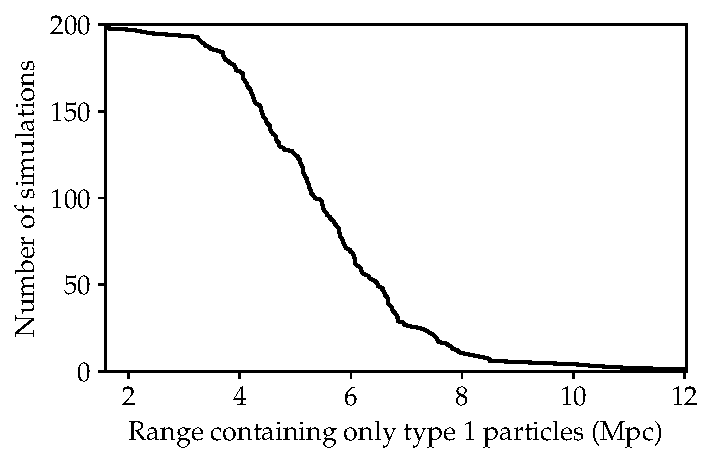
\includegraphics{kuvat/uncontaminatedDistances.pdf}
    \caption{Number of simulations that have only high resolution type 1 particles at least up to a given distance as a function of distance.}\label{fig:uncontaminatedDistances}
\end{figure}

\chapter{Mathematical and statistical methods}
täällä tarvittavat esitiedot ja önnönnöö, listaa mm. mitä aiot kertoa kunhan tiedät itsekään

\section{Statistical Background}
%\reversemarginpar
%\marginnote{\footnotesize{vähän parempi tässä kuin aiemman otsikon alla}}
%Precision of the used equipment limits accuracy of all data gathered from physical experiments, simulations or observations. Therefore the results are affected by the measurement process and the results have to be presented as estimates with some error, magnitude of which is affected by both number of data points and accuracy of the measurement equipment \citep{bohm2010introduction}.

Precision of the used equipment limits accuracy of all data gathered from physical experiments, simulations or observations. Thus assessing whether for example measurements support a model requires using statistical methods. The main methods relevant for this thesis are covered here. The methods are shortly introduced in the following sections together with basic statistical concepts that are necessary to understand the methods. 

%Estimating errors for measured quantities offers a way to test hypotheses and compare different experiments \citep{bohm2010introduction}. 
%This is done using different statistical methods, of which the main methods relevant for this thesis are covered here. The methods are shortly introduced in the following sections together with basic statistical concepts that are necessary to understand the methods. 


\subsection{Hypothesis testing and p-values}
A common situation in scientific research is that one has to compare a sample of data points to either a model or another sample in order to derive a conclusion from the dataset. In statistics, this is known as hypothesis testing \citep{wall2003practical}. For example, this can mean testing hypotheses such as ``these two variables are not correlated'' or ``this sample is from a population with a mean of 1.0''. Next paragraphs shortly introduce the basic concept of hypothesis testing and methods that can used to test the hypothesis ``these two samples are drawn from the same distribution'' following the approach of \citet{bohm2010introduction} and \citet{wall2003practical}.

The process of hypothesis testing as described by \citet{bohm2010introduction} begins with forming a null hypothesis $H_0$ that is formatted such that the aim for the next steps is to either reject it or deduce that it cannot be rejected with a chosen significance level. The negation of the null hypothesis is often called research hypothesis or alternative hypothesis and denoted as $H_1$. For example, this can lead to $H_0$ ``this dataset is sampled from a normal distribution'' and $H_1$ ``this dataset is not sampled from a normal distribution''. Choosing the hypotheses in this manner is done because often the research hypothesis is difficult to define otherwise.

After setting the hypothesis one must choose an appropriate test statistic. Ideally this is chosen such that the difference between cases $H_0$ and $H_1$ is as large as possible. Then one must choose 
the significance level $\alpha$ which corresponds to the probability of rejecting $H_0$ in the case where $H_0$ actually is true. This fixes the critical region i.e.\ the values of test statistic that lead to the rejection of the $H_0$. This kind of probability based decision making is always prone to error. Rejecting $H_0$ despite it being true is known as error of the first kind. However, this is not the only kind of error possible. It might also occur that $H_0$ is false but it does not get rejected, which is known as error of the second kind.

%\reversemarginpar
%\marginnote{\footnotesize{kerro mikä $\alpha$ ja N käytössä myöhemmin kunhan tiedät}}
There is no one optimal way of choosing $\alpha$, but instead one should try to find a balance between false rejections of the null hypothesis and not being able to reject the null hypothesis based on the dataset even if it is false. When sample size (often denoted $N$) is large, smaller values of $\alpha$ can often be used as decisions get more accurate when $N$ grows. For example tässä työssä $\alpha$ oli jokin ja $N$ jotain muuta. TODO! %TODO

It is crucial not to look at the test results before choosing $\alpha$ in order to avoid intentional or unintentional fiddling with the data or changing the criterion of acceptance or rejectance to give desired results. Only after these steps should the test statistic be calculated. If the test statistic falls within the critical region, $H_0$ should be rejected and otherwise stated that $H_0$ cannot be rejected at this significance level. The critical values for different test statistics are widely found in statistical textbooks and collections of statistical tables or they can be calculated using statistical or scientific libraries available for many programming languages.

Despite statistical tests having a binary outcome ``$H_0$ rejected'' or ``$H_0$ not rejected'', a continuous output is often desired. This is what p-values are used for. The name p-value hints towards probability, but despite its name p-value is not equal to the probability that the null hypothesis is true. These p-values are functions of a test statistic and the p-value for a certain value $t_{obs}$ of a test statistic gives the probability that under the condition that $H_0$ is true, the value of a test statistic for a randomly drawn sample is at least as extreme as $t_{obs}$. Therefore, if the p-value is smaller than $\alpha$, $H_0$ is to be rejected.

\subsection{Distribution functions} \label{sect:distribution-functions}
%\reversemarginpar
%\marginnote{\footnotesize{ei hyvä, harkitse esim http://puppu\-lause\-generaattori.fi/?ava\-in\-sana=ja\-kau\-ma\-funk\-tio}}
Some statistical tests such as the Kolmogorov-Smirnov test and the Anderson-Darling test make use of distribution functions such as cumulative density function (CDF) and empirical distribution function (EDF) in determining the distribution from which a sample is drawn. %Therefore it is important to grasp these concepts in order to fully understand these tests. [this is shit t. puppe]

To understand CDF and EDF, one must first be familiar with probability density function (PDF).
%\reversemarginpar
%\marginnote{\footnotesize{PDF määritelmä vaikea ymmärtää}}[0.5cm]
As the name suggests, a PDF is a function the value of which at some point $x$ represents the likelihood that the value of the random variable would equal $x$. This is often denoted as $f(x)$. Naturally for continuous functions the probability of drawing any single value from the distribution is zero, so these values should be interpreted as depicting relative likelihoods of different values. For example if $f(a)=0.3$ and $f(b)=0.6$ we can say that drawing value $b$ is twice as likely as drawing value $a$. \citep{htk}

Another way to use the PDF is to integrate it over a semi-closed interval from negative infinity to some value $a$ to obtain the CDF, often denoted with $F(x)$:
\begin{equation}
	F(x) = \int_{-\infty}^x f(x') \,dx'.
\end{equation}	
This gives the probability of a random value drawn from the distribution having value that is smaller than $x$. The relation between the PDF and the CDF is illustrated in Fig.\ \ref{fig:cdf}, where PDFs and CDFs are shown for three different distributions. It is easy to see the integral relation between PDF and CDF and how wider distributions have wider CDFs. \citep{htk}

\begin{figure}
%   \reversemarginpar
%	\marginnote{\footnotesize{lisää johonkin selitys normaalijakauman parametreille}}
   \centering
   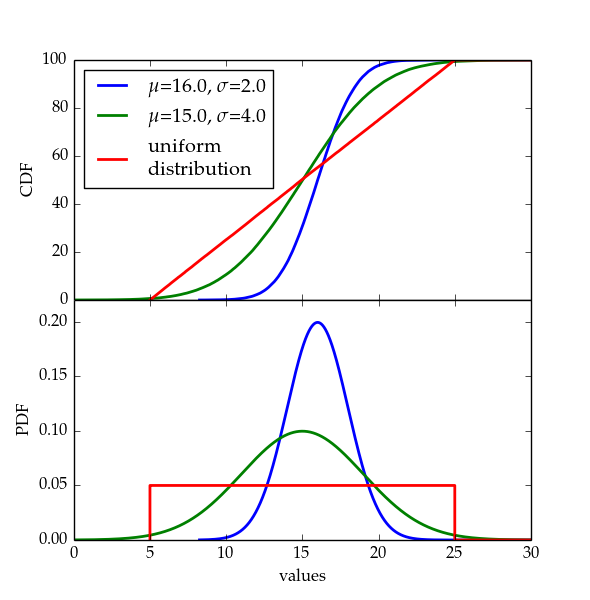
\includegraphics[width=0.9\textwidth]{kuvat/cdf.png}
   \caption{Cumulative distribution functions (top panel) and probability distribution functions (bottom panel) for three random samples drawn from different distributions, two of which are normal and one is uniform. Parameters $\mu$ and $\sigma$ of the normal distribution describe the mean and the spread of the distribution respectively, large values of $\sigma$ corresponding to a wide distribution.}
   \label{fig:cdf}

\end{figure}

%\reversemarginpar
%\marginnote{\footnotesize{esittelet nyt nolosti EDF:n nimeltä kahdesti, mieti ratkaisu}}
Both the PDF and the CDF apply to whole populations or to the sets of all possible outcomes of a measurement. In reality the sample is almost always smaller than this. Therefore one cannot measure the actual CDF. Nevertheless, it is possible to calculate a similar measure of how big a fraction of measurements falls under a given value. This empirical counterpart of the CDF is known as empirical distribution function (EDF), often denoted $\hat F(x)$, and for a dataset $X_1, X_2,\,..., X_n$ containing $n$ samples it is defined to be
\begin{equation}
	\hat F(x) = \frac{1}{n}\sum_{i=1}^n I[X_i \leq x]
\end{equation}
where $I$ is the indicator function, value of which is 1 if the condition in brackets is true, otherwise 0. \citep{feigelson2012modern}

%\reversemarginpar
%\marginnote{\footnotesize{harkitse laittavasi jämpti arvo N:lle kun muut osat valmiita}}
Due to the EDF being a result of random sampling, it may deviate from the underlying CDF considerably as can be seen by comparing CDFs in Fig.\ \ref{fig:cdf} and corresponding EDFs in Fig.\ \ref{fig:edf}. This example is somewhat exaggerated with its $N$=35 as the actual dataset used in this thesis has $N$>100, but reducing the sample size makes seeing the effects of random sampling easier. The latter figure also has EDFs corresponding to two random samples drawn from the distribution of the green curve in the first figure to further illustrate the differences that can arise from random sampling. This randomness also makes determining whether two samples are drawn from the same distribution difficult.

\begin{figure}
   \centering
   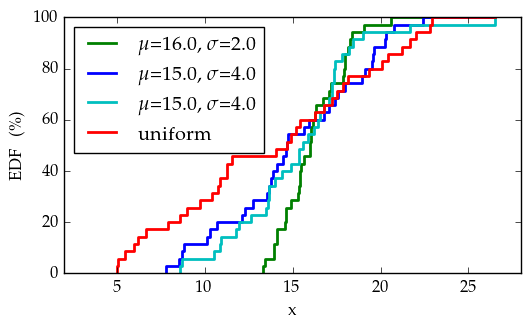
\includegraphics[width=0.9\textwidth]{kuvat/edf.png}
   \caption{Empirical distribution function for four random samples ($N$=35) drawn from the same distributions as in Fig.\ \ref{fig:cdf}. Note that both the blue and the cyan data are drawn from the same distribution.}
   \label{fig:edf}
\end{figure}


\section{Linear Regression}
Regression analysis is a set of statistical analysis processes that are used to estimate functional relationships between a response variable (denoted with $y$) and one or more predictor variables (denoted with $x$ in case of single predictor or $x_1 \dots x_i$ if there are multiple predictor variables) \citep{feigelson2012modern}. In this section, we will cover both simple regression, where there is only one response variable, and multiple linear regression, where there are more than one predictor variables. The models also contain an $\varepsilon$ term that represents the scatter of measured points around the fit. One of the models used is the linear regression model, which can be used to fit any relationship where the response variable is a linear function of the model parameters \citep{montgomery2012introduction}. In addition to the widely known and used models where the relationship is a straight line, such as $y = \beta_0 x + \varepsilon$, 
%\begin{equation}
%	y = \beta_0 x + \varepsilon
%\end{equation}
all models where relationship is linear in unknown parameters $\beta_i$ are linear \citep{montgomery2012introduction}. Thus for example $y = \beta_0 x^2 + \varepsilon$ and $y = \beta_0 e^x + \beta_1 \tan{x} + \varepsilon$ are linear models.
%\begin{align}
%	y &= \beta_0 x^2 + \varepsilon \\
%	y &= \beta_0 e^x + \beta_1 \tan{x} + \varepsilon \\
%	y &= \beta_0 + \beta_1 x_1 + \beta_2 x_2 + \varepsilon.
%\end{align}
On the other hand, all models where the relationship is not linear, for example $y = x^{\beta_0} + \varepsilon$ and $y = \beta_0 x + \cos{(\beta_1 x)} + \varepsilon$,
%\begin{equation}
%	y = x^{\beta_0}+ \varepsilon
%\end{equation}
%and
%\begin{equation}
%	y = \beta_0 x + \cos{(\beta_1 x)} + \varepsilon,
%\end{equation}
are nonlinear.


\subsection{Simple linear regression}\label{sect:simple-linear}
%\reversemarginpar
%\marginnote{\footnotesize{onko otsikko järkevä kun }}
Simple linear regression is a model with a single predictor variable and a single response variable with a straight line relationship, i.e.
\begin{equation}
	y = \beta_0 + \beta_1 x + \varepsilon
\end{equation}
where parameter $\beta_0$ represents the $y$ axis intercept of the line and $\beta_1$ is the slope of the line \citep{montgomery2012introduction}. The parameters can be estimated using method of least squares, i.e. choosing parameter values that minimize the sum of squared differences between the data points and the fitted line \citep{montgomery2012introduction}. 

\begin{figure}
    \centering
    %\def\svgwidth{\columnwidth}
    \input{kuvat/tex/OLS.pdf_tex}
    \caption{Ordinary least squares fit (black line) to a data set (black circles) with the response variable on the vertical axis. The fitted line minimizes the sum of squares of vertical distances between the data points and the fitted line, shown in grey.}\label{fig:OLS}
\end{figure}

%\reversemarginpar
%\marginnote{\footnotesize{toisiko jotain lisää jos olisi $\beta_1$ ja $\beta_2$ lausekkeet?}}
The best-known method of minimizing the sum of squared error is the ordinary least squares (OLS) estimator. The OLS method uses differences in the response variable as shown in Fig.\ \ref{fig:OLS} and thus the minimized sum is
\begin{equation}
	\sum_{i=1}^n (y_i - \beta_0 - \beta_1 x_i)
\end{equation}
where $x_1$ and $y_i$ are single values of the measured quantities \citep{feigelson2012modern}. This approach requires that the values of the predictor variable are known exactly without error and all uncertainty is in the values of the response variable \citep{feigelson2012modern}. In those situations where this assumption is not valid, results acquired using OLS may be counterintuitive. This can be seen for example in Fig.\ \ref{fig:OLSproblem} where OLS is used to calculate two linear fits: one where $x$ is used and predictor variable and $y$ as response variable and another where $y$ is the predictor and $x$ the response. As the minimized distance is different, the fitted lines also differ.

\begin{figure}
    \centering
    %\def\svgwidth{\columnwidth}
    \input{kuvat/tex/OLSproblem.pdf_tex}
    \caption{Ordinary least squares fits using either vertical or horizontal distances, both resulting in different fit. In order to avoid such ambiquity, ordinary least squares should only be used when the predictor variable is measured exactly.}\label{fig:OLSproblem}
\end{figure}

%\reversemarginpar
%\marginnote{\footnotesize{HF: OLS/TLS? Sido PCA:han}}
When dividing the variables to the independent variable with no error and a response variable with possible measurement error is not a justifiable choice, OLS should not be used. For example when fitting the Hubble flow to observations, both observed distances and radial velocities are likely to contain some uncertainty and thus OLS is not an optimal choice. One alternative for OLS is total least squares (TLS, also known as orthogonal least squares in some sources such as \citet{feigelson2012modern}) regression can be used instead of OLS \citep{markovsky2007overview}.  The major difference between OLS and TLS is that instead of vertical distance, the minimized squared distance is measured between a point and its projection to the fitted line, thus providing minimum of the sum of the squared orthogonal distances from the line \citep{feigelson2012modern}. These minimized distances are shown in Fig.\ \ref{fig:TLS}.

\begin{figure}
    \centering
    %\def\svgwidth{\columnwidth}
    \input{kuvat/tex/TLS.pdf_tex}
    \caption{Total least squares minimizes the sum of squares of orthogonal distances of the data points from the fitted line. Distances between the data points (black circles) and the fitted line (black line) are shown in grey.}\label{fig:TLS}
\end{figure}



\subsection{Multiple linear regression}
%\reversemarginpar
%\marginnote{\footnotesize{gradun sovellus: onko PCR relevantti?}}
%ongelman kuvailu, esim OLS:lle yleistys, jälleen liittyy PCA


%\begin{equation}
%	\matr{y} = \matr{X}\matr{\beta} + \matr{\ varepsilon}
%\end{equation}
%where $y$ is the response variable, $x_i$ are the predictor variables

%Linear Regression Analysis : Theory and Computing
%Introduction to Linear Regression Analysis




%\subsection{Ordinary Least Squares}

%\subsection{


\section{Principal Component Analysis}
%\reversemarginpar
%\marginnote{\footnotesize{orthogonal vs uncorrelated}}
Principal component analysis (PCA) is a statistical procedure first introdueced by \citet{pearson1901lines} to aid physical, statistical and biological investigations where fitting a line or a plane to n-dimensional dataset is desired. When performing PCA, one transforms a data set to a new set of uncorrelated variables i.e.\ ones represented by orthogonal basis vectors. These variables are called principal components (PCs) \citep{jolliffe2002principal}. This approach also solves the problem of sometimes arbitrary choice of division of the data into dependent and independent variables introduced in section \ref{sect:simple-linear} \citep{pearson1901lines}. 

%\reversemarginpar
%\marginnote{\footnotesize{not sure if kannattaa kuvaille proseduuria erityisen tarkkaan, selityksestä tulee pitkällinen jos aikoo aloittaa keskimääräisen tähtitieteilijän lähtötasolta, ehkä vain ohjaa lähteeseen}}
PCA can be used to both reduce and interpret data \citep{johnson2007applied}. Often PCA alone does not produce the desired result, but instead PCs are used as a starting point for other analysis methods such as factor analysis or multiple regression \citep{johnson2007applied}. These applications are introduced in the following subsections together with a short description of performing PCA and interpreting its results. In addition to  these applications, PCA is also used in image compression, face recognition and other fields \citep{smith2002tutorial}.

\subsection{Extracting Principal Components}
\begin{figure}
    \centering
    \input{kuvat/tex/pca-illustrated.pdf_tex}
    \caption{Extracting the PCs of a two-dimensional data set. First the origin is moved to the centroid of the data, original location of which is shown with a red x in the top panel. Next the line along which the variance of the data points is largest is determined, shown with the black line in the middle panel. This is the first PC, to which the second PC is orthogonal and thus fully determined. In the bottom panel the data is plotted along these principal components.
    %First the centroid of the data set (the red x) is determined and the origin is moved to the centroid as is done in the middle panel. Next the first PC, i.e. the line along which the variance of the data points is largest, is determined, shown with the black line in the middle panel. The second PC is orthogonal to the first one, i.e. fully determined in the two-dimensional case. In the bottom panel, the data is plotted along these principal components.
    }\label{fig:pca-illustrated}
\end{figure}

In order to understand the process of obtaining principal components of a data set let us follow the procedure on a two-dimensional data set shown in the top panel of Fig.\ \ref{fig:pca-illustrated} with black dots. The first step of finding the PCs is to locate the centroid of the dataset i.e.\ the mean of the data along every axis \citep{smith2002tutorial}. This is marked with a red x in the top panel of Fig.\ \ref{fig:pca-illustrated}.

%\reversemarginpar
%\marginnote{\footnotesize{jos päädyt puhumaan eigenvektoreista tai kovarianssimatriiseista, selitä ne täällä}}
The best-fit line and therefore the PCs always pass through the centroid of the system \citep{pearson1901lines}, so subtracting the location of the centroid from the data is a natural next step, as this ensures that in the next step only the slope has to be determined. This is done in the middle panel of the Fig.\ \ref{fig:pca-illustrated}. If the variables have different units, each variable should be scaled to have equal standard deviations \citep{james2013introduction} unless the linear algebra based approach with correlation matrices, as explained in e.g. \citet{jolliffe2002principal}, is used.

If this scaling is not performed, the choice of units can arbitrarily skew the principal components. This is easy to see when considering for example a case where one has distances to galaxies in megaparsecs and their masses in units of $10^{12}\ \mathrm{M_{\astrosun}}$, both of which might result in standard deviations being of the order of unity and PCA might thus yield principal components that are not dominated by neither variable alone. Now, say another astronomer has a similar data set, but distances are given in meters. In this case, most of the variation is in the distances, so distances will also dominate the PCs. If all variables are measured in the same units, scaling can be omitted in some cases \citep{james2013introduction}.

Now the first PC can be located by finding the line that passes through the origin and has the maximum variance of the projected data points \citep{jolliffe2002principal}, shown with a black line in the middle panel of Fig.\ \ref{fig:pca-illustrated} for our data set. PCs are always orthogonal and intersect at the origin, so in the two-dimensional example case the second and final PC is fully determined. The data set can now be represented using the PCs as is shown in the bottom panel of the Fig.\ \ref{fig:pca-illustrated}.

For a data set with more than two dimensions, the second PC is chosen such that it and the first PC are orthogonal and that variance along the new PC is again maximised \citep{jolliffe2002principal}. This can be repeated for each dimension of the data set or, if dimensionality reduction is desired, only for a smaller number of dimensions.

%\reversemarginpar
%\marginnote{\footnotesize{mieti mitä monospeissillä ja ole konsistentti}}
This level of understanding is often enough to successfully apply PCA to a problem, because PCA has ready-made implementations for many programming languages such as \texttt{prcomp} in R \citep{james2013introduction} and \texttt{sklearn.decomposition.PCA} in the scikit-learn library  for Python \citep{scikit-learn}. If a more mathematical approach is desired, \citet{smith2002tutorial} explains PCA together with covariance matrices, eigenvectors and eigenvalues required to understand the process very clearly. \citet{jolliffe2002principal} also includes a very thorough description of PCA.


\subsection{Excluding Less Interesting Principal Components}
%\reversemarginpar
%\marginnote{\footnotesize{maininta bootstrappingista (loppuun?) ja siitä, että maistuu koneoppiminen?}}
Even though a data set has as many principal components as there are measured variables, one is often not interested in all of them as the last principal components might explain only a tiny fraction of the total variation in the data \citep{james2013introduction}. Reducing the dimensionality of the problem also greatly eases visualizing and interpreting the data. Thus one might want to retain only the first few PCs when PCA is used to, for example, compress, visualize or just interpret a data set \citep{james2013introduction, johnson2007applied}. Unfortunately, many of the rules and methods used to determine the number of PCs to retain are largely without a formal basis or require assuming a certain distribution which is often not justifiable with the data \citep{jolliffe2002principal}. With careful consideration these methods can nevertheless aid a researcher in making informed decisions and reasoned conclusions, so some rules are introduced in this section.

If the PCA is performed to aid visualizing the data set, retaining only the two first PCs can be a justified choice as two is the maximum number of dimensions that are easy to visualize on two-dimensional media such as paper and the two first PCs determine the best-fit plane for the data \citep{jolliffe2002principal}. Of course the question whether the two PCs are sufficient to describe the data reasonably well still remains unanswered in this case.

\begin{figure}
    \centering
    \input{kuvat/tex/scree.pdf_tex}
    \caption{Example of a scree plot of randomly generated normally distributed data. In this case the plot has a clear elbow at the fifth PC with the PCs 5-9 appearing roughly on a line. Thus the last four PCs could be omitted if dimensionality reduction is desired.}\label{fig:scree}
\end{figure}

One widely used technique was introduced by \citet{cattell1966scree} to be used in factor analysis, but is also very much applicable to PCA \citep{jolliffe2002principal}. This so called Cattell scree test involves plotting the variance of the data points along each PC versus the index of the PC. These plots tend to look similar to what is shown in Fig.\ \ref{fig:scree}, resembling a steep cliff with eroded material accumulated at the base, which is why these plots are known as scree plots and the nearly linear section of the plot is called the scree.

When the scree plot has two clearly different areas, the steep slope corresponding to the first PCs and a more gently sloping scree for the latter PCs, locating this elbow in the plot connecting the two areas will give the number of PCs that should be included \citep{jolliffe2002principal}, which in case of Fig.\ \ref{fig:scree} would yield five PCs. Some sources such as \citep{cattell1966scree} suggest that in some cases the PC corresponding to the elbow should be discarded, which will result in one less PC.

Unfortunately, as Cattell also acknowledges in his paper, all cases are not as easy to analyse as the one in Fig.\ \ref{fig:scree} and may prove difficult to discern for an inexperienced researcher. This problem might arise from for example noise in the linear part of the plot or the scree line consisting of two separate linear segments with different slopes. The first case has no easy solution, but in the latter case Cattell suggests using the smaller number of PCs.

%\reversemarginpar
%\marginnote{\footnotesize{joku kiva lopetus tämän jälkeen?}}
Another straightforward method for choosing how many PCs to retain is to examine how much of the total variation in data is explained by first PCs and including components only up to a point where pre-defined percentage of the total variance is explained \citep{jolliffe2002principal}. Whereas the previous method posed a challenge in determining which PC best matches the exclusion criteria, when using this approach the problem arises from choosing the threshold for including PCs. \citet{jolliffe2002principal} suggests that a value between 70~\% and 90~\% of the total variation is often a reasonable choice, but admits that the properties of the data set may justify values outside this range. Unfortunately, the suggested range is quite wide, so it may contain multiple PCs and therefore it is up to the researcher to determine the best number of PCs, while the criterion again acts only as an aid in the process. 



\subsection{Principal Component Regression}

\section{Error analysis}
% sources of error
% systematic error vs statistical uncertainty, only the second can be handled in this thesis
% bootstrapping + other methods


\section{Comparing two samples drawn from unknown distributions}
%\reversemarginpar
%\marginnote{\footnotesize{TODO: oispa parempi otsikko. mieti, onko tämä muutenkaan hyvä nyt kun on siirretty yksi otsikkotaso ylöspäin}}[-3cm]
A common question in multiple fields of science is whether two or more samples are drawn from the same distribution. The most relevant methods that can be used to address this problem are introduced here following \citet{bohm2010introduction} and \citet{feigelson2012modern} apart from introducing the $\chi^2$ test which is mostly based on the approach of \citet{corder2014nonparametric}.

Questions related to comparing samples can emerge for example when comparing effectiveness of two procedures, determining if the instrument has changed over time or whether observed data is compatible with simulations. There are multiple two-sample tests that can address this kind of questions, e.g. $\chi^2$, Kolmogorov-Smirnov, Cram\'er-von Mises and Anderson-Darling tests. 

In addition to comparing two samples, these tests can be used as one-sample tests to determine whether it is expected that the sample is from a particular distribution. However, some restrictions apply when using the one-sample variants. Some of these tests use categorical data, i.e. data where variables fall in pre-defined categories, and compares numbers of samples in different categories, whereas the others are applied to numerical data and compare empirical distribution functions (EDF) of the datasets.. Examples of such categories might be for example ``galaxies that are active'' or ``data points between values 1.5 and 1.6''.


\subsection{$\chi^2$ test}
%\reversemarginpar
%\marginnote{\footnotesize{keksi paremmat esimerkit koko kappaleeseen, jotain relevanttia myöhempää tutkimusta ajatellen. katso kommentit paperista sen jälkeen, kaikkia ei täällä vielä}}
Astronomical data often involves classifying objects into categories such as ``stars with exoplanets'' and ``stars without exoplanets'' or the spectral classes of stars  \citep{feigelson2012modern}. One tool for analysing such categorical data is $\chi^2$ test, which can be used both to determine whether a sample can be drawn from a certain distribution and to test whether two samples can originate from a single distribution. 

The method described here is sometimes referred to as Pearson's $\chi^2$ test due to existence of other tests where $\chi^2$ distribution is used. In some cases, such as with small $2 \times 2$ contingency tables and when expected cell counts are small, other variants of $\chi^2$ test should be used. For example the Yates's $\chi^2$ test or the Fisher exact test work better in these cases than the $\chi^2$ test.

For one-sample test, the $\chi^2$ test uses the number of measurements in each bin together with a theoretical estimate calculated from the null hypothesis. For example one might have observed exoplanets and tabulated the number of planet-hosting stars of different spectral class as is shown in Table \ref{tab:exoplanets} and now wants 
to test the observations against null hypothesis ``Distribution of stellar classes for observed exoplanet-hosting stars is equal to that of main sequence stars in solar neighbourhood as given by \citet{ledrew2001real}'' using significance level $\alpha=0.01$. The data is categorical, so now $\chi^2$ test is a justified choice.

\begin{table}
	\centering
	\begin{tabular}{p{2cm}|p{4cm}}
		Stellar class & Number of observed planetary systems \\ \hline
		A & 6 \\
		F & 38 \\
		G & 39 \\
		K & 134
	\end{tabular}
	\caption{Example of categorical data.}
	\label{tab:exoplanets}
\end{table}

\begin{table}
	\centering
	\begin{tabular}{ l | l | l }
		Stellar class & Observations ($f_o$)& Theory ($f_e$) \\ \hline
		A & 6 & 6 \\
		F & 38 & 28 \\
		G & 39 & 71 \\
		K & 134 & 112 \\ \hline
		total & 217 & 217
	\end{tabular}
	\caption{Data of Table \ref{tab:exoplanets} together with expected values if null hypothesis was true.}
	\label{tab:exoplanets-null}
\end{table}

In this case the first step would be to calculate the expected observation counts for each bin according to the null hypothesis. Table \ref{tab:exoplanets-null} contains these expected counts ($f_e$) together with the observations ($f_o$). These observed and expected values are then used to calculate the $\chi^2$ test statistic, defined as
\begin{equation}
	\chi^2 = \sum_i \frac{(f_o - f_e)^2}{f_e}.
\end{equation}
With the data given above this results in $\chi^2 \approx 23.6$. The data has four bins, so the degree of freedom is $4-1=3$. Next one can compare the calculated $\chi^2$ value to a tabulated critical value for our significance level $\alpha=0.01$. These tabulated values can be widely found in statistics textbooks and books specifically dedicated to statistical tables.

In this case according to \citet{corder2014nonparametric} the critical value is 11.34, which means that as $23.6>11.34$ one can reject the null hypothesis and conclude that at 1\% significance level the distribution of stellar classes for observed exoplanet-hosting stars is not equal to that of main sequence stars in solar neighbourhood. This of course can either be due to exoplanets being more numerous around some stellar classes than others or arise from some observational effect such as the observer observing more of the later type stars and thus arbitrarily skewing the distribution of the exoplanet finds.

The $\chi^2$ test can also be used to test for independence of two or more samples. The data is again tabulated and now the $\chi^2$ test statistic is calculated as
\begin{equation}
	\chi^2 = \sum_i \sum_j \frac{(f_{oij}-f_{eij})^2}{f_{eij}}
\end{equation}
where $f_{oij}$ denotes the observed frequency in cell $(i, j)$ and $f_{eij}$ is the expected frequency for that cell. The expected frequency can be calculated using the following formula
\begin{equation}
	f_{eij} = \frac{R_i C_i}{N}
\end{equation}
where $R_i$ is the number of samples in row $i$, $C_j$ is the number of samples in column $j$ and $N$ is the total sample size.

According to \citet{corder2014nonparametric}, the degrees of freedom is $(R-1)(C-1)$ where R is the number of rows and C is the number of columns in tabulated data. This is true in many if not most cases, but the way of collecting data can affect the degrees of freedom in both one-sample and multi-sample cases, as \cite{press2007numerical} explains. For example, if the one-sample model is not renormalized to fit the total number of observed events or, in two-sample case, the sample sizes differ, the degrees of freedom equal to number of bins $N_b$ instead of $N_b-1$.

Before performing the $\chi^2$ test on a dataset, it is important to confirm that the data meets the assumptions for $\chi^2$ test, given for example in \citep{bock2010stats} and \citep{htk}. First of all, the data has to consist of counts i.e.\ not for example percentages or fractions. These counts should be independent of each other and there has to be enough of them, generally $>50$ is sufficient. Bins should also be chosen such that all bins have at least five counts according to the null hypothesis. If the last condition is not met, one can can consider combining bins. 


\subsection{Kolmogorov-Smirnov test}
For astronomers, one of the most well-known statistical test is the Kolmogorov-Smirnov test, also known as the KS test. It is computationally inexpensive to calculate, easy to understand and does not require binning of data. It is also a nonparametric test i.e.\ the data does not have to be drawn from a particular distribution.

In the astrophysical context this is often important because astrophysical models usually do not fix a specific statistical distribution for observables and it is common to carry out calculations with logarithms of observables, after which the originally possibly normally distributed residuals  will no longer follow a normal distribution. When using the KS test, the values on the x-axis can be freely reparametrized: for example using $2x$ or $\log x$ on x-axis will result in same value of the test statistic as using just $x$ \citep{press2007numerical}.

The test can be used as either one-sample or two-sample test, both of which are very similar. For two-sample variate the test statistic for the KS test is calculated based on empirical distribution functions $\hat{F}_1$ and $\hat{F}_2$ derived from two samples and the test statistic
\begin{equation}
	D = \sup_{x} |\hat{F}_1(x) - \hat{F}_2(x)|
\end{equation}
uses the maximum vertical distance of the EDFs. This test statistic is then used to determine the p-value and thus decide whether the null hypothesis can be rejected. For one-sample variate the procedure is similar, but EDF $\hat{F}_2$ is substituted with the CDF that corresponds to the null hypothesis.

\begin{figure}
   \centering
   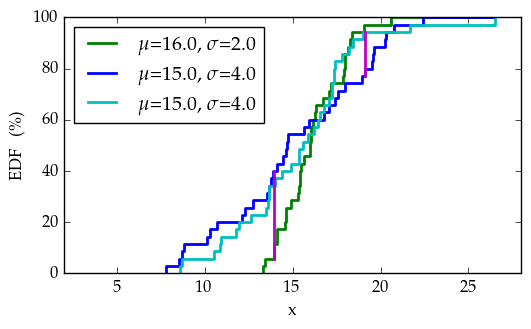
\includegraphics[width=0.9\textwidth]{kuvat/kstest.png}
   \caption{KS test parameter values (magenta vertical lines) shown graphically for three samples from Fig.\ \ref{fig:edf}.}
   \label{fig:ks} 
\end{figure}

As an example, let us consider two pairs of samples from Fig.\ \ref{fig:edf}: green and blue (two samples drawn from different normal distributions) and blue and cyan (two samples drawn from the same normal distribution). We can formulate the test and null hypotheses for both pairs as $H_0$=``the two samples are drawn from the same distribution'' and $H_1$=``the two samples are not drawn from the same distribution'' and choose a significance level of for example $\alpha=0.05$ or $\alpha=0.01$.

%\reversemarginpar
%\marginnote{\footnotesize{mistä p-value saadaan, kerro taas aiemmin (tai täällä)}}
The test statistic is then calculated and for these samples we get $D=0.51$ for the green-blue pair and $D=0.20$ for the blue-cyan pair. Test statistics are illustrated in Fig.\ \ref{fig:ks} where the test statistics $D$ are shown as vertical magenta lines. According to Python function \texttt{scipy.stats.ks\_2samp}, these values of $D$ correspond to p-values $9.9\times 10^{-5}$ and $0.44$ respectively, which means that the null hypothesis ``green and blue samples are drawn from the same distribution'' is rejected at both 0.05 and 0.01 significance levels but the null hypothesis ``blue and cyan samples are drawn from the same distribution'' cannot be rejected.

\begin{figure}
   \centering
   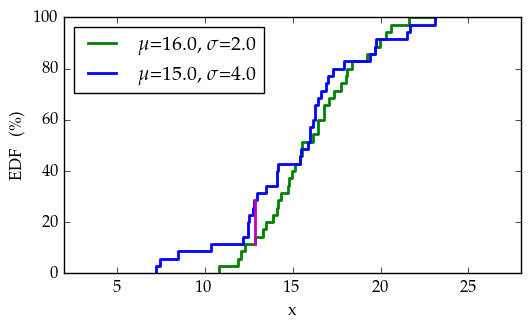
\includegraphics[width=0.9\textwidth]{kuvat/kstest-error.png}
   \caption{KS test ran on another pair of samples drawn from blue and green distributions in Fig.\ \ref{fig:cdf}.}
   \label{fig:ks-error} 
\end{figure}

In this case the KS test produced result that matches the actual distributions from which the samples were drawn. Using a different random realization might have resulted in a different conclusion, for example the one shown in Fig.\ \ref{fig:ks-error} results in $D=0.17$ that corresponds to a p-value of $0.64$ i.e.\ null hypothesis could not have been rejected using the $\alpha$ specified earlier. In a similar manner there can be cases where two samples from one distribution are erroneously determined not to come from the same distribution if the samples differ from each other enough due to random effects.

The latter example case also illustrates one major shortcoming of the KS test: it is not very sensitive to small-scale differences near the tails of the distribution. For example in Fig.\ \ref{fig:ks-error} the blue sample goes much further left, but because EDF is always zero at the lowest allowed value and one at the highest one the vertical distances near the tails are small and the test is most sensitive to differences near the median value of the distribution. On the other hand, the test performs quite well when the samples differ globally or have different means. \citep{feigelson2012modern}

%\reversemarginpar
%\marginnote{\footnotesize{"explain better"}}[1.8cm]
The KS test is also subject to some limitations and it is important to be aware of them in order to avoid misusing it. First of all, the KS test is not distribution free if the model parameters, e.g. mean and standard deviation for normal distribution, are estimated from the dataset that is tested. Thus the tabulated critical values can be used only if model parameters are determined from some other source such as a simulation, theoretical model or another dataset.

Another severe limitation of KS test is that it is only applicable to one-dimensional data. If the dataset has two or more dimensions, there is no unique way of ordering the points to plot EDF and therefore if KS test is used, it is no longer distribution free. Some variants that can handle two or more dimensions have been invented, such as ones by \citet{peacock1983twodimensional} and \citet{fasano1987multidimensional}, but the authors do not provide formal proof of validity of these tests. Despite this, the authors claim that Monte Carlo simulations suggest that the methods work adequately well for most applications.

% mutlidimensionaaleista http://articles.adsabs.harvard.edu/cgi-bin/nph-iarticle_query?1987MNRAS.225..155F&defaultprint=YES&filetype=.pdf ja http://articles.adsabs.harvard.edu/cgi-bin/nph-iarticle_query?1983MNRAS.202..615P&defaultprint=YES&filetype=.pdf


\subsection{Other tests based on EDFs}
%\reversemarginpar
%\marginnote{\footnotesize{ehkä vähän lyhyenpuoleisia kappaleita}}
Unsatisfactory sensitivity of the KS test motivates the use of other more complex tests. Such tests are for example the Cram\'er-von Mises test (CvM) and Anderson-Darling (AD) test, both of which have their strengths. Similar to KS test, both of these can be used as one-sample or two-sample variants.  

First of these tests integrates over the squared difference between the EDF of the sample and CDF from the model or two EDFs in case of two-sample test. The test statistic $W^2$ for one-sample case can be expressed formally as
\begin{equation}
	W^2 = \int_{-\infty}^{\infty}[\hat F_1(x) - F_0(x)]^2\ dF_0(x)
\end{equation}
For two-sample version, the theoretical CDF $F_0$ has to be replaced with another empirical distribution function $\hat F_2$.

Due to integration, the CvM test is able to differentiate distributions based on both local and global differences, which causes it to often perform better than the KS test. Similar to the KS test, the CvM test also suffers from EDFs or an EDF and a CDF being equal at the ends of the data range, which again makes the test less sensitive to differences near the tails of the distribution. 

In order to achieve constant sensitivity over the entire range of values, the statistic has to be weighted according to the proximity of the ends of the distribution. The AD test does this with its test statistic defined as
\begin{equation}
	A^2 = N \int_{-\infty}^{\infty} \frac{[\hat F_1(x) - F_0(x)]^2}{F_0(x)[1-F_0(x)]}\ dF_0(x)
\end{equation}
where $N$ is the number of data points in sample. This weighing makes the test more powerful than the KS and CvM tests in many cases. \citep{bohm2010introduction, feigelson2012modern}

%\reversemarginpar
%\marginnote{\footnotesize{hnnngh}}
Also other more specific tests exist, such as the Kuiper test which is well suited for cyclic measurements. The test should always be chosen to match the dataset such that it best differentiates between the null and research hypotheses.

\section{Cluster Analysis}
The aim of cluster analysis is to find groups of similar data points within a data set, these groups being called clusters \citep{han2000data}. Ideally data points within each cluster are as similar to each other as possible and dissimilar to data points outside the cluster \citep{han2000data}. It has many applications in multiple fields ranging from machine learning to biology and it can also be applied in astronomy and astrophysics to e.g. classify objects and possibly even discover new ways to classify them \citep{ball2010data, han2000data}. For example \citet{mukherjee1998three} were able to divide gamma ray bursts to three distinct categories separated by a combination of their durations, brightnesses and spectra.

The definition of a cluster is intentionally loose, allowing the exact definition to vary between problems to which it is applied \citep{tan2006introduction}. Differences can arise for example from whether one data point can be part of multiple clusters and whether all data points should be part of some cluster or if the dataset contains noise not belonging to any cluster. Many different algorithms have been developed for performing cluster analysis, each best suited for some specific type of data \citep{han2000data}. The algorithm used should always be chosen based on the desired properties of the clusters and the properties of the data set.

One clustering algorithm that is well suited for finding clusters based on a density threshold in a spatial data set is DBSCAN, originally presented by \citet{ester1996density}. It produces a density-based clustering, meaning that the identified clusters consist of data points residing in high-density regions, each cluster separated from others by a low-density region \citep{han2000data}. This definition allows both finding clusters of arbitrary shape and working with noisy data with data points that do not belong to any cluster \citep{ester1996density}.

The algorithm uses two parameters defining the properties of the clusters: $\varepsilon$ (sometimes denoted Eps) and MinPts. The $\varepsilon$ parameter resembles the linking length used by the \textsc{fof} algorithm introduced in section \ref{sect:halofinding} as it sets the size of the neighbourhood used when determining whether a data point is part of a cluster. The distance function can be chosen freely to best fit the problem, possible metrics being e.g. Euclidean or Manhattan distance. The points within the distance $\varepsilon$ from a given data point are said to belong to its $\varepsilon$\=/neighbourhood. This definition implies that a data point also belongs to its own $\varepsilon$\=/neighbourhood.

If more than MinPts data points belong to the $\varepsilon$\=/neighbourhood of a data point, it belongs to a cluster and is defined to be a core point of that cluster. If a core point has another core point in its $\varepsilon$\=/neighbourhood, the two core points belong to the same cluster. For example in Fig.\ \ref{fig:DBSCAN-twocores} the red points are all core points of one cluster, but as no blue points are within $\varepsilon$\=/neighbourhood of any red point, the blue points form their own cluster. When MinPts = 2, the resulting clustering is identical to one produced by the \textsc{fof} algorithm.

\begin{figure}
    \centering
    %\def\svgwidth{\columnwidth}
    \input{kuvat/tex/DBSCAN-twocores.pdf_tex}
    \caption{An example data set shown as dots, surrounded by circles showing the extent of $\varepsilon$\=/neighbourhoods of each data point. To reduce clutter, all but one $\varepsilon$\=/neighbourhood border are shown in grey. When MinPts = 4, the data points are separated to two clusters, shown in red and blue here. As every point has at least four data points within its $\varepsilon$\=/neighbourhood, all data points are core points.}\label{fig:DBSCAN-twocores}
\end{figure}

Some points might belong to an $\varepsilon$\=/neighbourhood of a core point but have $\varepsilon$\=/neighbourhoods with less than MinPts data points in them. These points are border points and they are also members of the cluster containing the core point in the $\varepsilon$\=/neighbourhood of the border point. For example in Fig.\ \ref{fig:DBSCAN-borderpoint} the light blue border point belongs to the cluster defined by the dark blue core points. Cluster membership does not propagate further from border points, meaning that e.g. the grey data point next to the light blue point in Fig.\ \ref{fig:DBSCAN-borderpoint} is not part of any cluster despite belonging to the $\varepsilon$\=/neighbourhood of one of the cluster members as this member is a border point.

\begin{figure}
    \centering
    %\def\svgwidth{\columnwidth}
    \input{kuvat/tex/DBSCAN-borderpoint.pdf_tex}
    \caption{A single cluster with MinPts = 4 and $\varepsilon$ shown with circles. The dark blue points all have at least four points in their $\varepsilon$\=/neighbourhood so they are core points, but the light blue point has an $\varepsilon$\=/neighbourhood of only three points. Thus despite it being part of the $\varepsilon$\=/neighbourhood of a core point, it is not a core point. Instead, it is a border point of the cluster. The grey point in the $\varepsilon$\=/neighbourhood of the light blue point does not have four points in its $\varepsilon$\=/neighbourhood nor does it belong to an $\varepsilon$\=/neighbourhood of any core point, so it is not part of the cluster. Similarly none of the other grey points have enough particles in their neighbourhoods so they do not belong to any cluster.}\label{fig:DBSCAN-borderpoint}
\end{figure}

In a situation where a border point is in $\varepsilon$\=/neighbourhoods of core points belonging to different clusters, as happens for example to the grey data point in Fig.\ \ref{fig:DBSCAN-ambiquity}, it is not clear to which cluster the border point should be assigned. The density-based definition of a cluster presented by \citet{ester1996density} would classify these border points to all clusters whose core points reside in the $\varepsilon$\=/neighbourhoods of these border point. Often a clustering with each data point belonging to a maximum of one cluster is desired instead, so the DBSCAN algorithm classifies this kind of border points only to the first cluster they are discovered in. 

This introduces some possibly unexpected behaviours. First of all, while the algorithm is deterministic when run multiple times on the same data set, the clustering is dependent on the order of the data points \citep{schubert2017dbscan}. If the order of data points is permuted, the cluster to which these border points between two clusters are assigned might change. Fortunately this is a fairly rare occasion and the effects of assigning a single border point to one cluster or another are often insignificant \citep{schubert2017dbscan}.

\begin{figure}
    \centering
    %\def\svgwidth{\columnwidth}
    \input{kuvat/tex/DBSCAN-ambiquity.pdf_tex}
    \caption{In this situation the grey data point could belong to either red or blue cluster. The DBSCAN algorithm will be added to the cluster that is discovered first, so depending on the order of the data points it might be part of either red or blue cluster.}\label{fig:DBSCAN-ambiquity}
\end{figure}

Another edge case is even more extreme. Consider the configuration of data points is Fig.\ \ref{fig:DBSCAN-singlecore} where the $\varepsilon$\=/neighbourhood of the grey point contains one border point from each of the three other clusters. As these are only border points, the grey point is not member of any of the three coloured clusters, but its $\varepsilon$\=/neighbourhood has four points, so it is a core point of its own. Now assuming that the red, blue and yellow clusters are all found before the grey point is processed, the grey data point becomes the core point of a cluster containing only a single data point. These clusters with fewer than MinPts members are of course even rarer than the occasions when the cluster membership of a border point is ambiguous, as they require border points of multiple clusters stretching close to the core area of a small cluster without merging with it. Even with these fairly rarely occurring undesirable features, the DBSCAN algorithm is in many cases more robust than the \textsc{fof} algorithm, as choosing an approppriately large value of MinPts for example reduces the probability of a thin bridge of data points connecting otherwise separate clusters.

\begin{figure}
    \centering
    %\def\svgwidth{\columnwidth}
    \input{kuvat/tex/DBSCAN-singlecore.pdf_tex}
    \caption{Another clustering with MinPts = 4. One border point from red, blue and yellow clusters each resides within the $\varepsilon$\=/neighbourhood of the grey point, but as these are border points (shown with lighter colours), the grey point belongs to none of the other clusters. The grey point has four points in its $\varepsilon$\=/neighbourhood, making it a core point. If the three other clusters are discovered before the cluster membership of the grey data point is determined, it becomes the only data point of its own cluster.}\label{fig:DBSCAN-singlecore}
\end{figure}

The properties of the identified clusters naturally depend on the used parameters $\varepsilon$ and MinPts. Different heuristics exist for determining suitable values for them. For MinPts, \citet{schubert2017dbscan} provide a value of twice the dimensionality of the dataset, e.g. for two dimensional data MinPts = 4 should be chosen. For some datasets a higher value can be better if the dataset for example contains duplicate data points or is very large or high-dimensional \citep{schubert2017dbscan}.

According to \citet{ester1996density}, $\varepsilon$ can be set after choosing the value of MinPts by inspecting the distances of data points to their $k$\textsuperscript{th} nearest neighbour. Here $k$ can be set to the same value as MinPts, though the results do not seem to vary greatly if $k$ is increased \citep{ester1996density}. When the $k$\=/distances are sorted in descending order and plotted, the resulting plot often shows an elbow similar to the one in the scree plot in Fig.\ \ref{fig:scree}. Examples of such plots can be seen in Fig.\ \ref{fig:k-distances-singlesim} that shows $k$\=/distance plots for six different values of $k$ ranging from 2 to 7. \citet{ester1996density} suggest that the distance corresponding to the elbow should be used as a value of $\varepsilon$, with the points to the left of the elbow corresponding to noise. The location of the elbow is usually not very sensitive to small changes in $k$, as can be seen in Fig.\ \ref{fig:k-distances-singlesim} where the location of the elbow changes less than 0.1 radians over the six different values of $k$. If domain knowledge is available, $\varepsilon$ and MinPts can also be chosen differently to best suit the data set \citep{schubert2017dbscan}.

\begin{figure}
    \centering
    %\def\svgwidth{\columnwidth}
    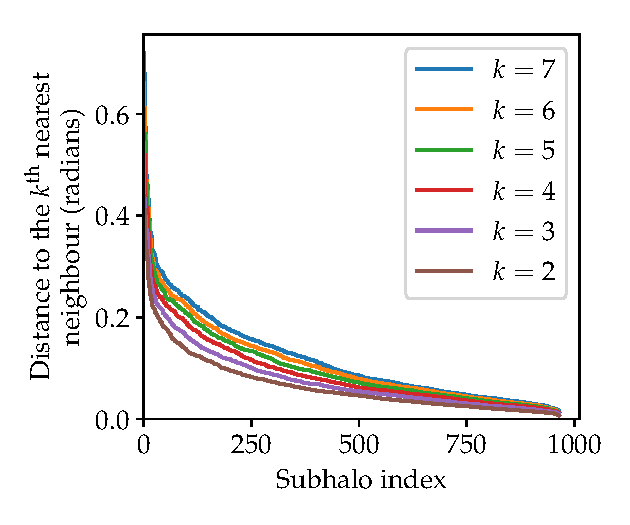
\includegraphics{kuvat/k-distances-singlesim.pdf}
    \caption{Six $k^{\text{th}}$ nearest neighbour distance plots with $k$ ranging from 2 to 7. Variations in the location of the elbow are reasonably small when $k$ is varied.}\label{fig:k-distances-singlesim}
\end{figure}


\chapter{Findings from Halo Catalogue Analysis}
TODO intro %TODO

\section{Properties of the Local Group analogues}
As the Local Group analogue identification criteria described in section \ref{sect:zooms} allow for a range of different halo pairs, the properties of the found Local Group analogues vary. This can be seen in Fig. \ref{fig:LGproperties} where both distance between the main haloes and the velocity components span nearly the whole allowed range of values. The plot also contains a histogram of overdensity within 2 Mpc of the Milky Way analogue.

\begin{figure}
    \centering
    %\def\svgwidth{\columnwidth}
    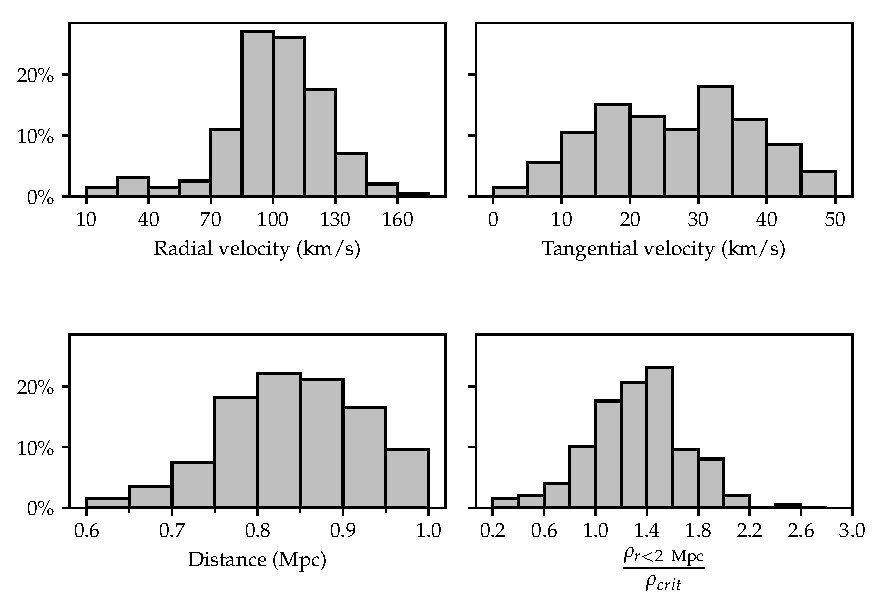
\includegraphics{kuvat/LGproperties.pdf}
    \caption{Histograms of the mutual radial and tangential velocities (top row) and distances (bottom left panel) of the main haloes in each Local Group analogue found in the simulations. The bottom right panel shows the overdensity within 2 Mpc of the Milky Way analogue in each simulation. The densities are calculated based on the combined mass of subhaloes, so the values of overdensity are somewhat smaller than they would be if all mass within 2~Mpc was included.}\label{fig:LGproperties}
\end{figure}

The peak of the radial velocity histogram is located near 100 km/s, meaning that most of the identified Local Group analogues have radial velocities near the measured value for the Andromeda galaxy \citep{vandermarel2012m31}. Pairs with low radial velocity are rare, as according to the timing argument in order to have a radial velocity close to zero the mass of the Local Group would typically have to be small, which is excluded by the mass criterion used. For tangential velocities, the distribution is much more uniform, though values near the ends of the allowed interval are still fairly rare. The \citet{vandermarel2012m31} tangential velocity measurement result of 17.0~km/s would also fall in one of the densely populated bins, though the tangential velocity measurements have much larger uncertainties than radial velocities: the $1\sigma$ confidence region extends to 34.3~km/s, covering more than half of the allowed range in the Local Group analogue identification criterion \citep{vandermarel2012m31}.

Modern distance estimates for M31 range from 770 to 800 kpc with errors of few tens of kpc, meaning that the distance is slightly shorter than in most of the simulated Local Group analogues but still near the peak of the distribution \citep{mcconnachie2005distances}. Analogues with shorter distances between the primaries are somewhat rare whereas distances at the longer end of the allowed range are more common. This is likely an effect of the mass and radial velocity criteria together with the fact that a spherical shell of constant thickness has larger volume on larger distances and thus if a constant probability density function is assumed also more subhaloes.

As can be seen in the overdensity histogram, most of the Local Group analogues are located in an overdense region. Densities in the histogram only include the mass within subhaloes, so the total densities within the examined 2~Mpc regions is somewhat larger. There is also a small number of Local Group analogues in very underdense regions. This is possible only if the primary haloes are on the lower end of the allowed mass range, they have only low mass satellites and there are no other comparable structures within the 2~Mpc distance. Very high density regions are also rare as they require either a large number of smaller haloes or a halo with a mass comparable to the primaries of the Local Group to fall within the 2~Mpc region.

The combined mass of the primaries in the Local Group analogues and its distribution between the haloes also varies from simulation to simulation. This is illustrated in Fig. \ref{fig:LGmasses} that shows the mass of the more massive of the primaries in each simulation against the combined mass of the pair. The allowed range of the masses is outlined with the grey lines, the lower one showing the threshold where the more massive halo holds exactly half of the total mass and the upper one illustrating the maximum possible mass in the more massive halo when the Local Group analogue criteria require the smaller one to have a mass of at least $4 \times 10^{11}~\mathrm{M_{\astrosun}}$.

\begin{figure}
    \centering
    %\def\svgwidth{\columnwidth}
    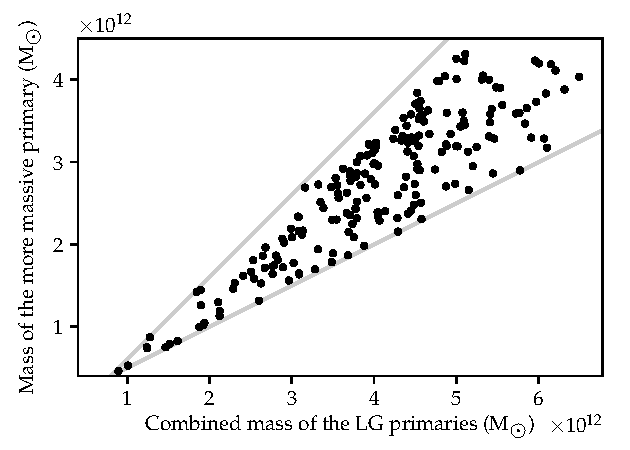
\includegraphics{kuvat/LGmasses.pdf}
    \caption{The masses of the more massive primary plotted against the combined mass of the primaries, each black dot representing one Local Group analogue. Grey lines show the allowed range: the more massive one has to contain at least half of the combined mass and the smaller one has to have a mass of at least $4 \times 10^{11}~\mathrm{M_{\astrosun}}$.}\label{fig:LGmasses}
\end{figure}

There are Local Group analogues both with almost equal masses and with the smaller halo barely exceeding the minimum mass, though as can be seen in the figure, the former case is more common. Especially for total masses larger than $2 \times 10^{12}~\mathrm{M_{\astrosun}}$ the area near the upper limit for the mass of the more massive primary is nearly vacant of data points. This is likely caused by environments with density high enough for them to be able to host the more massive primary usually having other massive subhaloes in them too. Thus in dense environments it is common that more than one halo with a mass larger than that of the smaller primary is present within the 2~Mpc distance used to check that the two primaries are the dominant haloes in their surroundings.

\begin{figure}
    \centering
    %\def\svgwidth{\columnwidth}
    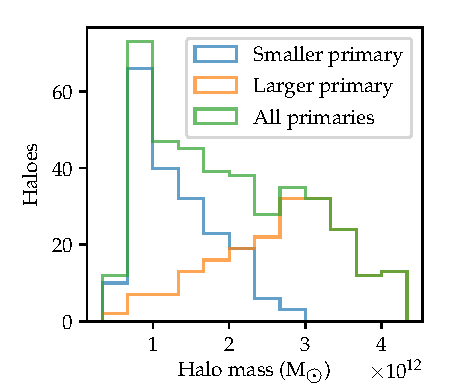
\includegraphics{kuvat/masshistogram.pdf}
    \caption{Histograms showing the masses of the identified Local Group analogue primaries. The blue and yellow histograms contain only the less or more massive subhalo of each primary respectively whereas the green histogram shows the masses of all subhaloes in a primary pair of a Local Group analogue.}\label{fig:masshistogram}
\end{figure}

The Local Group identification criteria allow the combined mass of the primaries between $8 \times 10^{11}~\mathrm{M_{\astrosun}}$ and $1 \times 10^{13}~\mathrm{M_{\astrosun}}$, but whereas the lower end of the range is populated, there are no Local Group analogues with combined mass of $7 \times 10^{12}~\mathrm{M_{\astrosun}}$ or more. This is likely because high mass haloes are relatively rare in the sample: only about one fifth of all haloes in a primary pair of a Local Group analogue have a mass of more than $3 \times 10^{12}~\mathrm{M}_{\astrosun}$. This is illustrated in Fig.~\ref{fig:masshistogram} that shows histograms of masses both separately for the smaller and larger primary in each pair and all primaries together. It can also be seen that the masses do not span the full allowed range, as the most massive subhalo in a Local Group analogue has a mass of $4.3 \times 10^{12}~\mathrm{M}_{\astrosun}$, % 4.31347031218e+12 M_sun
clearly below the maximum allowed mass of $5 \times 10^{12}~\mathrm{M}_{\astrosun}$. It is notable how the distribution of the masses of the larger haloes in the primary pairs extends all the way to the lowest masses whereas there are no primary pairs with the mass of the smaller halo exceeding $3 \times 10^{12}~\mathrm{M}_{\astrosun}$. % sum(allhalomasses > 3e12)*1.0/len(allhalomasses) = 0.20351758794

Overall, the 199 Local Group analogues chosen from the zoom simulations span a wide range of different two-halo systems. Only the values near the very edges of the allowed ranges in each variable are rare. This allows an analysis of correlations of the mass of the system with its other properties.


\section{Hubble Flow Measurements}
The Local Group analogues analysed in this project do not only differ in the properties of the primaries but also in the environments in which they reside. The primaries can for example have few or many satellites around them and the velocity dispersion within the system can vary. Similarly, the volume further out from the system can be densely populated with haloes possibly arranged in filaments or walls, or the Local Group analogue can be located in a very low density environment. These environmental factors are explored in this section and a way to quantify a selection of them for further analysis is presented.

\subsection{Different Hubble Flows}

\begin{figure}
    \centering
    %\def\svgwidth{\columnwidth}
    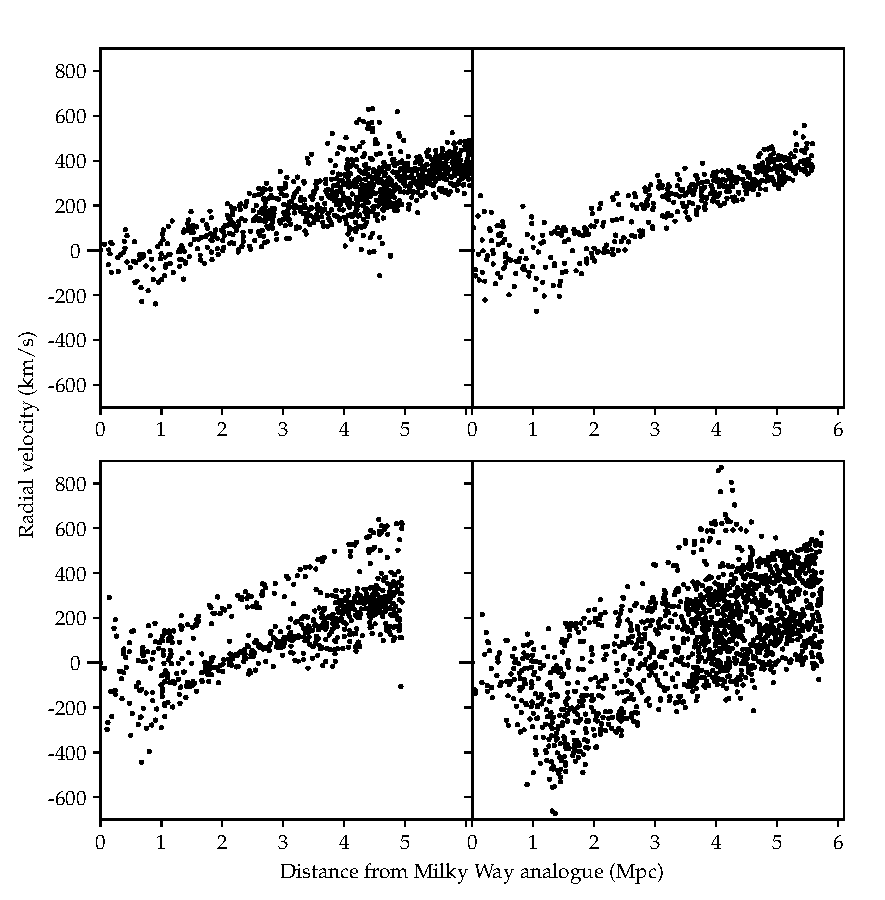
\includegraphics{kuvat/hubblediagrams.pdf}
    \caption{Hubble flows around Milky Way analogues in four simulations differing in for example the total number of subhaloes, scatter of the flow, scatter within the Local Group and the number of bound structures present within the flow. Each black dot represents one subhalo in a simulation and subhaloes are drawn up to the distance at which the first type 2 particle resides.}\label{fig:hubblediagrams}
\end{figure}

A selection of these different environments is illustrated in Fig.~\ref{fig:hubblediagrams} showing radial velocities as seen from the lower mass primary plotted against the distance of the subhalo. This corresponds to what a Hubble diagram would look like as seen from the Milky Way analogue of that simulation. Each of the four panels contains all subhaloes in that simulation up to the closest type 2 particle. The simulations shown in this plot are chosen such that they show a variety of different Hubble Flows, but naturally four simulations can never show the full range of all 199 analysed simulations nor all structures that can occur.

The simulations on the top row in Fig.~\ref{fig:hubblediagrams} both show fairly small dispersion of radial velocities at each distance, corresponding to a cold Hubble flow. In the upper left plot, there is a region with a much larger velocity dispersion between approximately 4 and 5~Mpc, likely corresponding to a massive subhalo surrounded by satellite galaxies, some of which are receding and some approaching the observer as they orbit the primary or primaries of the system. The upper right plot on the other hand shows no such variation in the velocity dispersion, apart from the dispersion within the nearest 1~Mpc or so being higher than in the rest of the plot due to the velocities of the satellite galaxies within the Local Group analogue, whereas the upper left plot has fairly low velocity dispersion within the Local Group.

The simulations presented in the bottom row of the figure show considerably higher velocity dispersions. Especially the bottom right plot, with radial velocities in it easily spanning a range of 400~km/s at all distances except within 1~Mpc of the Milky Way analogue, differs from the top row plots. The bottom right plot also has a much greater number of subhaloes than the other plots. The bottom left plot, on the other hand, seems to show a Hubble flow that is divided into two parts with a vertical offset of around 100~km/s. This kind of situation might occur, for example, if the Local Group analogue is moving relative to the surrounding structures.

These kinds of differences in the surroundings of the Local Group analogues might be correlated with the mass of the primaries and could thus provide a way to gauge the mass of the real Local Group by observing its surroundings. These correlations are explored in section \ref{sect:statistical_estimate}, but in order to conduct statistical analysis, the properties of the Hubble flow have to be quantified first.


\subsection{Measuring the Hubble Flow} \label{sect:hubblemeasurement}
The first step in quantifying the properties of the Hubble flows around the Local Group analogues is to determine the basic shapes of each flow. In this work, the radial velocity field is modelled as consisting of two parts: at small distances when going outward from the Milky Way analogue, the radial velocity decreases or perhaps stays nearly constant with a possibly large scatter, and at larger radii a positive linear relationship between distance and radial velocity is expected. Naturally this is not an exact description of the situation, as the transition from a gravitationally bound Local Group analogue to a linear Hubble flow is not instantaneous and the gravitational pull of the Local Group also affects objects outside it.

Fitting a linear relation to the linear Hubble flow observed around the Milky Way analogues is, in principle, simple, as for example the ordinary least squares regression (see section \ref{sect:simple-linear}) can be used. Determining the distance from which the linear model can be applied, on the other hand, is less straightforward and multiple possible schemes exist. Possibly the simplest option would be to set an arbitrary distance threshold and exclude all haloes within this distance from the fitting procedure. For some simulations, this will likely exclude more data points than is necessary and for others it is possible that not enough points will be excluded. Even when the exclusion threshold is chosen carefully, in a large sample a constant distance will always be suboptimal for some simulations, so a solution that is able to adapt to the properties of each simulation is desired.

\begin{figure}
    \centering
    %\def\svgwidth{\columnwidth}
    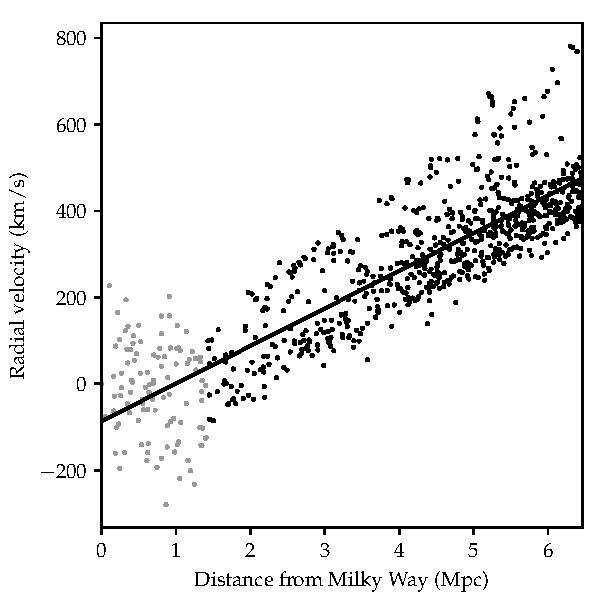
\includegraphics{kuvat/hubblefit.pdf}
    \caption{Hubble flow fit (black line) calculated by excluding a number of innermost subhaloes resulting in the smallest mean squared residual. For this simulation, this was achieved when excluding the first 1.4~Mpc of haloes, producing a measured Hubble flow slope of 87.0~km/s/Mpc. The excluded subhaloes are shown as grey points and subhaloes used to fit the Hubble flow as black dots.}\label{fig:hubblefit} %86.9929348817 km/s/Mpc, 1.43211533035 Mpc
\end{figure}

When not otherwise stated, in this work the number of nearest subhaloes to be ignored is chosen based on the sum of squares of the residuals. This is done by finding the number of innermost subhaloes up to 2~Mpc away from the Milky Way analogue to be ignored in order to get the smallest mean squared residual for the ordinary least squares fit. The final result of this kind of fitting procedure is illustrated in Fig.~\ref{fig:hubblefit}, where all subhaloes are shown as dots: the excluded ones in grey and ones used in fitting in black. The best fit line is also shown. In this simulation the excluded range corresponds well to the distinction a human would likely make when asked to determine the distance at which the motions inside Local Group are no longer the dominant effect on the radial velocity.

This approach is naturally not without weaknesses. For example if the innermost subhaloes within Local Group have a very small radial velocity dispersion, no subhaloes might be excluded as a large number of data points with small dispersion can reduce the mean squared residual even if they skew the result. Similarly groups of data points with large scatter can get excluded even if they otherwise follow the Hubble Flow neatly. Luckily these problems are usually not severe as even when the maximum of 2 Mpc of the nearest region is excluded from fitting, most simulations still have more than 3~Mpc worth of data to use for fitting and thus small changes in including or excluding subhaloes in the innermost regions do not produce large effects. This is also confirmed in the following subsection where the dependence of Hubble flow parameters on the distance are explored.

%The fitting is also repeated multiple times for each simulation, making the procedure slow compared to e.g. the case with a constant exclusion threshold. Adaptive solutions with possibly better time complexities also exist, as one might for example calculate the fit iteratively by always excluding the haloes that are closer than the distance at which the fitted radial velocity is zero. This is an appealing approach as instead of just the scatter around the fit the result is based on the physical distance at which the Hubble flow can be said to start. Unfortunately the solution does not necessarily converge but can instead oscillate between two or more solutions. Also the range starting at the point where the fitted radial velocity is zero can in some simulations contain a substantial number of subhaloes with large velocity dispersion that are likely to be bound to the Local Group. Due to the disadvantages of the faster methods and the fact that the slower method is fast enough to be used with the data set at hand, the slower method comparing the mean squared residuals was chosen for this work.

When the results of the fitting are expressed in this work, the Hubble flow fitting result is not expressed in the most familiar slope-intercept form of $y = kx + b$ giving the slope and the $y$ intercept. Instead the result is expressed in terms of the Hubble flow slope $H_0$ and the distance at which the fitted radial velocity is zero, corresponding to giving the $x$ intercept instead of $y$. This convention is chosen as the zero point indicates the distance at which subhaloes are no longer bound to the Local Group, which in turn can be used to probe the mass of the Local Group. Sometimes the velocity dispersion of the Hubble flow is also interesting. In order to calculate it, the Hubble flow fit is first subtracted from the radial velocities, after which the velocity dispersion is obtained by taking the standard deviation of the differences.


\subsection{Dependence of the Hubble Flow Parameters on Distance}
The distance from the Milky Way analogue to the nearest type 2 particle varies from simulation to simulation as was seen in Fig.~\ref{fig:uncontaminatedDistances} in section~\ref{sect:zooms}. The range of closest to furthest distance to the nearest type 2 particle is also quite substantial: the closest particle can be closer than 2 Mpc away from the Milky Way analogue but some simulations contain only type 1 particles in a spherical volume with radius of more than 10~Mpc. Thus if the Hubble flow measurements were very sensitive to the distance up to which data is available, simulations might appear to have different Hubble flows just because they are measured up to different distances.

\begin{figure}
    \centering
    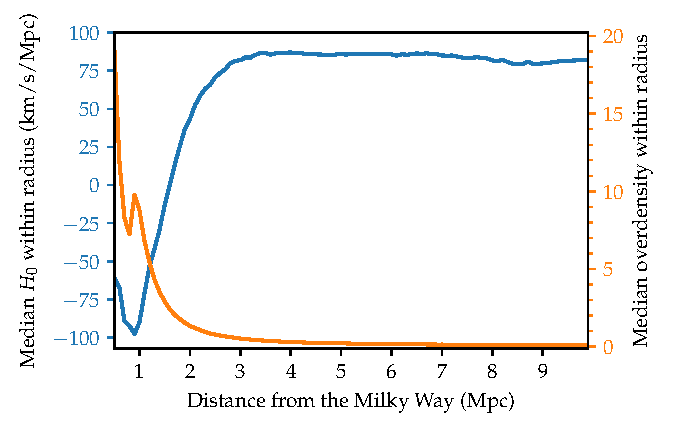
\includegraphics{kuvat/overdensity+H0.pdf}
    \caption{Median $H_0$ results (blue curve) and overdensities (orange curve) in the simulation sample up to a given radius. The plot shows clearly how both of the values evolve within the Local Group, including the effect of the M31 and its satellites, and how the values stabilize at larger radii. The overdensity is measured using only mass contained in subhaloes and thus at large distances it tends to a value smaller than unity. At each radius the plot only contains simulations that are free of type~2 particles up to that distance, so the last measured values are medians of values from very few simulations.}\label{fig:overdensity+H0}
\end{figure}

The possibility of this affecting the results of Hubble flow measurements is explored in Fig.~\ref{fig:overdensity+H0}, the blue curve of which shows the median value of Hubble flow slope $H_0$ when all haloes within a given radius are used to construct an ordinary least squares fit. As the closest subhaloes are also a part of the data used in fitting, the fits done only based on the nearest haloes produce negative values of $H_0$. The smallest values are seen at the radius where the M31 analogues reside in the simulations, produced by the M31 and its satellite system moving towards the Milky Way. Moving the exclusion threshold further out, the measured values of $H_0$ grow as more and more of the actual Hubble flow is included until at approximately 3~Mpc the median value reaches a maximum and no longer changes.

The same plot also includes a curve showing the median overdensity within a radius, mass being measured as the combined mass of all subhaloes with a centre of potential within the given distance from the Milky Way. Near the Milky Way the overdensity is large but it decreases when the examined volume grows until M31 is reached, at which point the median overdensity rises again, showing a bump in the curve. After this the decrease in density continues until after 3~Mpc there is very little mass belonging to subhaloes compared to the  volume. As the mass only contains mass enclosed in subhaloes, at large radii the overdensity does not tend to one but to a smaller value.

The two curves in Fig.~\ref{fig:overdensity+H0} correspond to each other neatly: at regions with high overdensity structures are gravitationally bound and $H_0$ measurements yield negative values and, at larger distances, as the overdensity decreases the values of $H_0$ rise closer to the global value in the simulation. At very large distances of more than 7~Mpc the $H_0$ curve shows slight variations, but as there are only few simulations that are free of type 2 particles up to those distances, these are likely not actual features but instead produced by local variations in the Hubble flow of possibly as few as a single simulation.

It is also notable that the measured median value of $H_0$ rises to a value of more than 80~km/s/Mpc, i.e. clearly higher than the global value of 67.77~km/s/Mpc for the simulations. This can happen as the Local Group analogue selection criteria also places indirect restrictions on the surroundings of the system. This effect can also possibly be used when determining the mass of the Local Group.

As the point after which the measured median value for $H_0$ no longer changes is reached fairly soon, it seems that e.g. 5~Mpc region containing only type~1 particles is sufficient for obtaining a reasonably reliable estimate of the shape of the Hubble flow surrounding the Local Group analogue. This is important for further statistical analysis as only a small fraction of the simulations is free of type 2 particles up to for example 7~Mpc whereas more than half of the simulations still contain only type 1 particles within 5~Mpc.

\begin{figure}
    \centering
    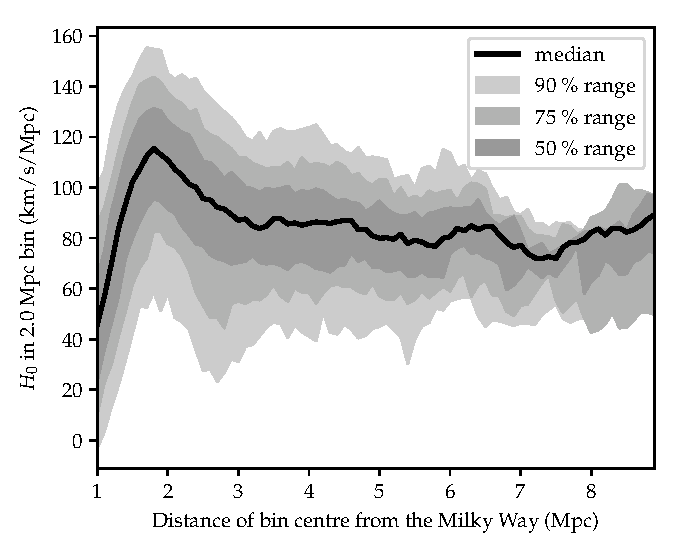
\includegraphics{kuvat/shelledH0.pdf}
    %\input{kuvat/tex/shelledH0.pdf_tex}
    \caption{Median $H_0$ when fitted in all subhaloes with distances from the Milky Way analogue in a 2~Mpc bin. The grey areas show ranges containing the middle 90\%, 75\% and 50\% of the measurements. The value of $H_0$ is calculated only for bins that do not contain any type 2 particles, which results in the total number of data ponints decreasing outwards. For approximately the last megaparsec, the small number of available data points causes the 90\% and 75\% limits merging.}\label{fig:shelledH0}
\end{figure}

As the $H_0$ values shown in Fig.~\ref{fig:overdensity+H0} include all subhaloes up to a given distance, they  differ from values obtained as described in section~\ref{sect:hubblemeasurement}. The plot also does not give  any insight into whether the observed relation between distance and radial velocity in simulations is linear or not. In order to examine these effects, Fig.~\ref{fig:shelledH0} shows how the median $H_0$ changes as a function of distance when measured using all haloes in a moving 2~Mpc bin. The plot also shows the extents of the ranges containing the middle 90\%, 75\% and 50\% of the $H_0$ values in each bin. The merging of different ranges at large radii is caused by the plot including in each bin only those simulations that do not have type~2 particles in that bin, so there are very few data points in the last bins.

Like Fig.~\ref{fig:overdensity+H0}, this plot also shows how initially the values of $H_0$ grow when the bin moves away from the Milky Way analogue, but the curve reaches a significantly higher value of $H_0$ than the curve in Fig.~\ref{fig:overdensity+H0}. This is caused by the bin including both M31 and its satellites moving towards the Milky Way analogue and haloes outside the Local Group moving away, which results in the measured $H_0$ being exaggerated. At larger distances the measurement no longer has haloes bound to the Local Group analogue in it and it stabilizes to a value near the one in Fig.~\ref{fig:overdensity+H0}.

As the unbinned figure, Fig.~\ref{fig:shelledH0} also starts to show some variation in the value of $H_0$ near a distance of 7~Mpc for the bin centre. This is also likely at least partially related to the number of simulations from which the median is calculated getting smaller, but actual features in the data set can also affect the result. For example massive haloes moving relative to the Milky Way and hosting their own satellite systems can also result in anomalous values of $H_0$ when the distance range used in the measurement is small.

\begin{figure}
    \centering
    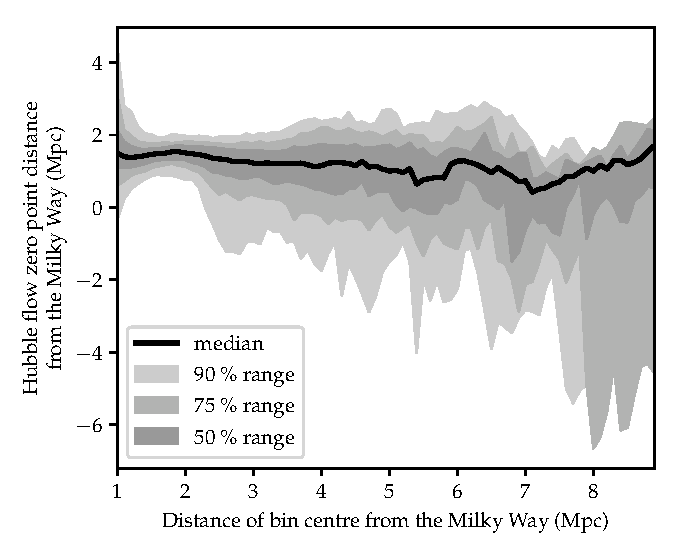
\includegraphics{kuvat/zeros.pdf}
    %\input{kuvat/tex/zeros.pdf_tex}
    \caption{Median Hubble flow zero point distance from the Milky Way analogue, measured from a Hubble flow fitted to all subhaloes in a 2 Mpc bin in each simulation, accompanied with the ranges containing the middle 90\%, 75\% and 50\% of the measurements. As in Fig.~\ref{fig:shelledH0}, the zero point is calculated only in bins that do not contain type 2 particles and thus for large distances there are less measurements, resulting in the 90\% and 75\% ranges merging.}\label{fig:shelledZeros}
\end{figure}

%Mpc	uncontaminated sims
%0	199
%1	199
%2	198
%3	194
%4	173
%5	125
%6	69
%7	27
%8	11

% # of data points in each bin:
% [197 197 197 197 197 196 196 196 195 195 194 193 193 193 192 190 188 188
% 184 176 171 167 162 159 153 150 144 143 137 134 129 126 115 108 107 103
%  93  88  85  81  77  69  62  59  52  48  43  37  37  35  31  28  26  21
%  20  20  18  17  16  15  14  13  13  12  11  11  11  10   9   8   7   7
%   6   6   6   6   6   6   6   6]

In addition to the measured value of $H_0$, the zero point of the fitted Hubble flow can also change if the distance range within which the fit is calculated changes. This is explored in Fig.~\ref{fig:shelledZeros} showing how the Hubble flow zero point changes if it is measured from a fit to all haloes with radial distances in a 2~Mpc bin and the bin centre is moved. Unlike $H_0$, the zero point does not change drastically based on whether M31 analogue and its satellites are inside the bin limits. This is likely caused by the steepening of the fitted line getting cancelled out by the data to which the line is fitted being further from the origin. 

This plot also suggests that a volume with a relatively small radius of e.g. 5~Mpc or even less is sufficient to gain good fitting results, as there does not seem to be any systematic change in the zero point at large distances. As this result is compatible with the conclusions drawn from Figs.~\ref{fig:overdensity+H0} and \ref{fig:shelledH0}, a maximum distance of 5~Mpc is adopted for the Hubble flow fitting using the procedure described in the previous subsection. This allows using a constant upper limit for the range used in fitting while still being able to use more than half of all Local Group analogues in the analysis and without losing the accuracy of the fitting.

As with the $H_0$ plots, the zero point measurement results also vary more on larger distances. When looking at the plotted ranges, it is clear that in the outermost bins the scatter is very large. Even ``negative distances'' to the zero point are present, meaning that the fit would suggest that even the Local Group is expanding. These kinds of results are possible when the data set used in fitting no longer contains subhaloes that are bound to the Local Group analogue and the slope of the fitted line is more gradual and closer to the global value of 67.77~km/s/Mpc, at which point the zero point can move close to the Milky Way analogue or if the $H_0$ is very small even to ``negative'' distances. This means that the fit is no longer sensitive to the overdensity within the Local Group. Especially when only distant haloes are used, the negative radial velocities within the Local Group might not affect the fit significantly.




\section{Anisotropy of Hubble flow}
isotropy + randomness or anisotropy? esittele konsepti. plots: see notebook last pages

%\reversemarginpar
%\marginnote{\footnotesize{Simulaatio 97, esittele jo tässä näkyvät klöntit joissa paljon samaa väriä, näytä myös klusterointi ja vertaa löytöjä siihen}}
Figure \ref{fig:mollweide-anisotropy} shows distribution of haloes around Milky Way analogue from one simulation with haloes closer than 1.5 Mpc away from center excluded to avoid cluttering the view with Andromeda counterpart and its satellites.

\begin{figure}
    \centering
    %\def\svgwidth{\columnwidth}
    \input{kuvat/tex/mollweide-anisotropy.pdf_tex}
    \caption{Projections of haloes around the less massive LG primary with distances ranging from 1.5 Mpc to 5.0 Mpc.}\label{fig:mollweide-anisotropy}
\end{figure}

\begin{figure}
    \centering
    \input{kuvat/tex/directionalHF.pdf_tex}
    \caption{Mean Hubble flow slope and zero point as seen from Milky Way analogue in different 20\textdegree\ bins as measured from line connecting Milky Way and Andromeda analogues, direction 0\textdegree\ being towards Andromeda. From each simulation bins with less than 10 subhaloes in them were excluded, total 25.}\label{fig:directionalHF}
\end{figure}

\begin{figure}
    \centering
    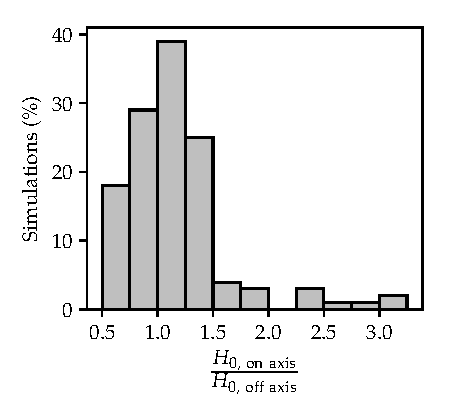
\includegraphics{kuvat/directionalHF-ratios.pdf}
    \caption{Ratio of $H_0$ measurements from subhaloes near the line connecting the Milky Way and M31 analogues to ones far from that line. On axis haloes are defined as ones that form an angle of less than 45\textdegree\ with the line as seen from Milky Way analogue.}\label{fig:directionalHF}
\end{figure}

\subsection{Clustering}
Used DBSCAN introduced in [earlier chapter], angular distances of projections on sky as seen from MW.

Figure \ref{fig:clusteringparameters} shows the effect of varying minsamples and $\varepsilon$ on number of clusters found in each simulation (1.5 Mpc < r < 5.0 Mpc again). Regions where there are ridiculously many clusters and ones where there are one or zero, relevant region in between, some areas have similar number of clusters but do the clusters look the same, see plots that don't exist yet

\begin{figure}
    \centering
    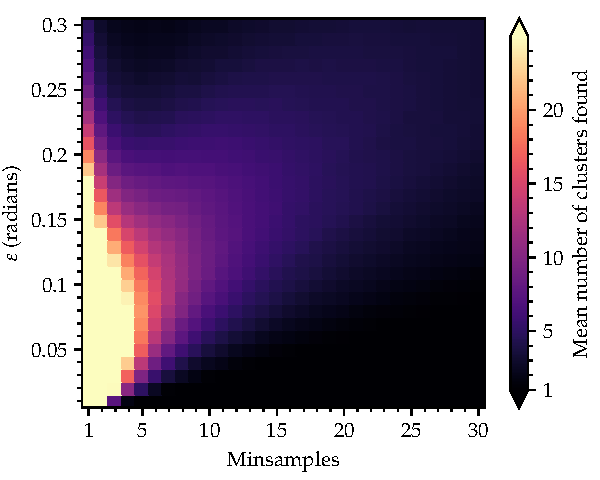
\includegraphics{kuvat/clusteringParameters.pdf}
    \caption{Mean number of clusters found for all simulations in dataset with different DBSCAN parameters.}\label{fig:clusteringparameters}
\end{figure}

%\reversemarginpar
%\marginnote{\footnotesize{TODO: mieti laitatko samaan figureen, vertaile kuitenkin, selitä vasemmanpuolimmainen pikselisarake}}
Figure \ref{fig:clusterdiameter} shows the change in mean diameter (supremum of angular distance between haloes) in cluster when $\varepsilon$ and minsamples are varied. White areas where no clusters are found in any simulation.

\begin{figure}
    \centering
    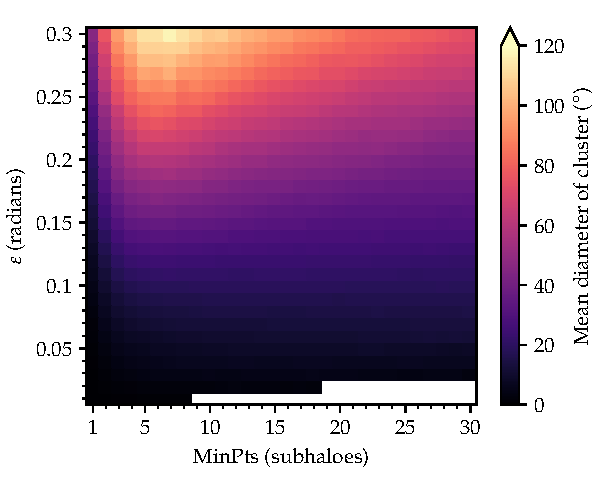
\includegraphics{kuvat/clusterDiameter.pdf}
    \caption{Mean diameter of clusters found for all simulations in dataset with different DBSCAN parameters.}\label{fig:clusterdiameter}
\end{figure}

\begin{figure}
    \centering
    \input{kuvat/tex/4-distances.pdf_tex}
    \caption{Sorted 4-dist graphs for subhaloes between $1.5$ and $5.0$ Mpc from the Local Group in each simulation that is uncontaminated at least up to 5 Mpc from the Local Group. The plotted distances are measured as the angular distance between the subhaloes as seen from the Milky Way analogue. %eps 0.17, ehkä alempikin, esim 0.15 %TODO
    }\label{fig:4-distances}
\end{figure}

%\reversemarginpar
%\marginnote{\footnotesize{Ehkä vähän vähemmän tilaa plottien välissä vaakasuunnassa? Keltaiset vähän turhan samanlaisia.}}
Figures \ref{fig:clusteringExamples} and \ref{fig:clusteringvariations} show how the clustering results vary when clustering parameters are varied.

\begin{figure}
    \centering
    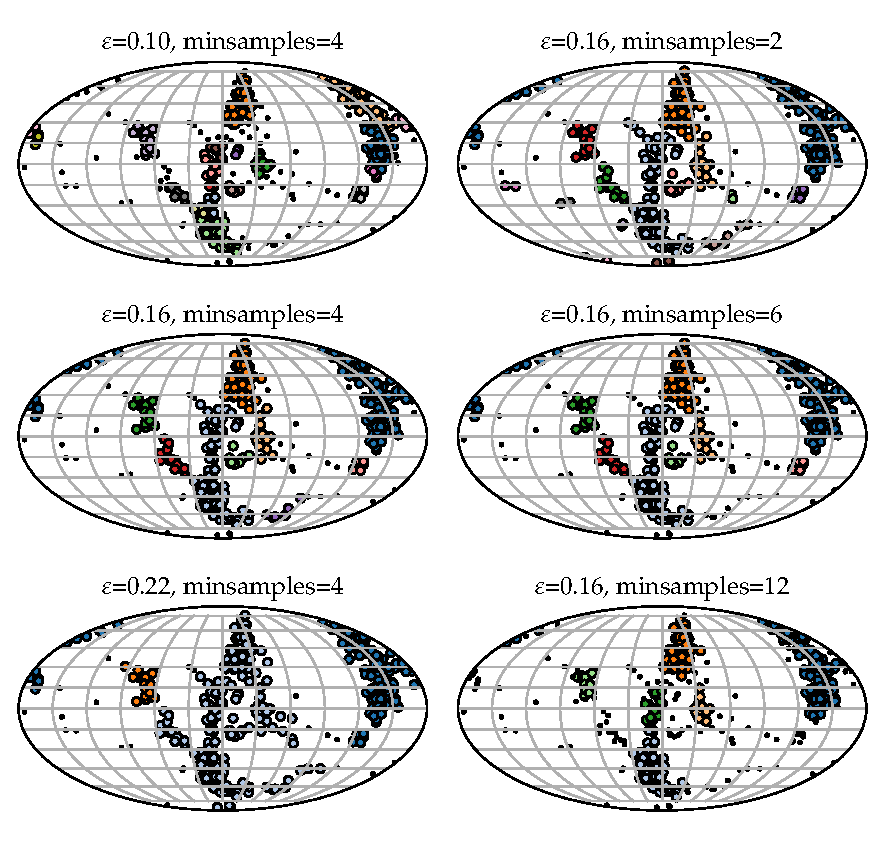
\includegraphics{kuvat/clusteringExamples.pdf}
    \caption{Results of DBSCAN clustering on same simulation output with different clustering parameters. TODO: erittele parametrien muuttamisen vaikutukset}\label{fig:clusteringExamples}
\end{figure}

\begin{figure}
    \centering
    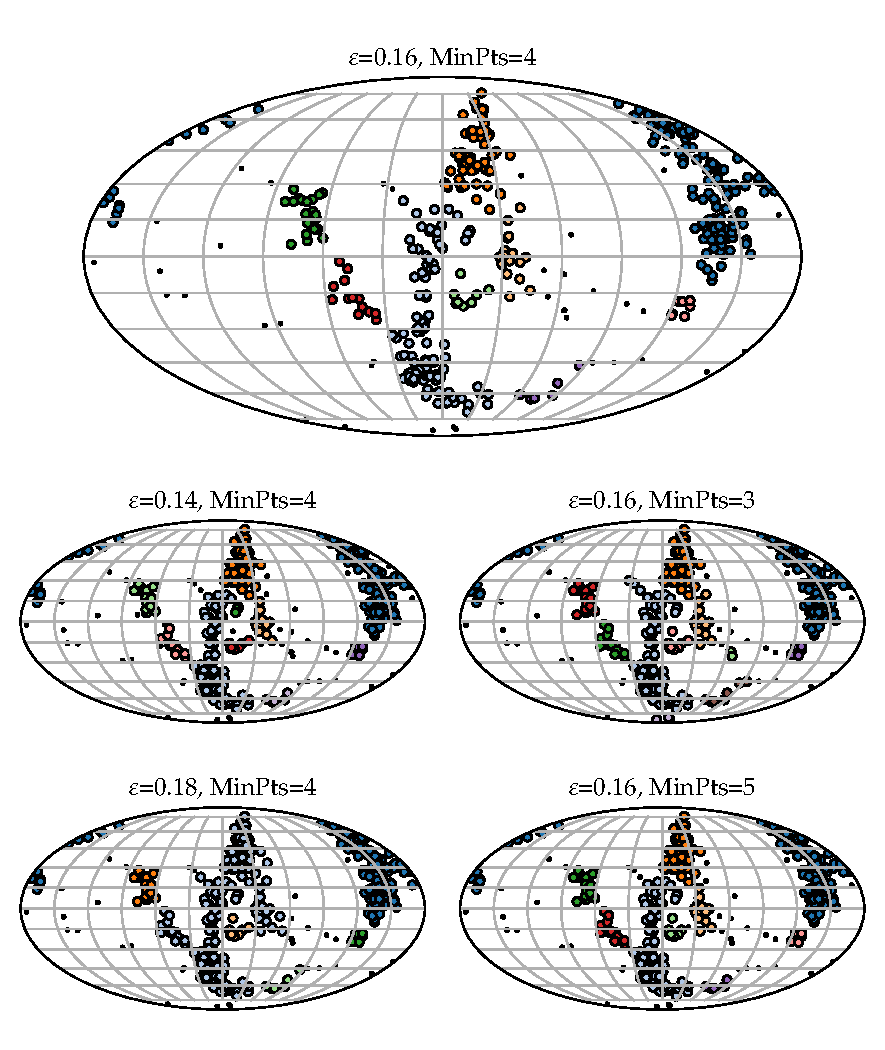
\includegraphics{kuvat/smallClusteringVariations.pdf}
    \caption{The effect of slightly variying the clustering parameters around the values $\varepsilon$=0.16 and minsamples=4 used when analysing clustered data. TODO: more sensitive to $\varepsilon$}\label{fig:clusteringvariations}
\end{figure}

\begin{figure}
    \centering
    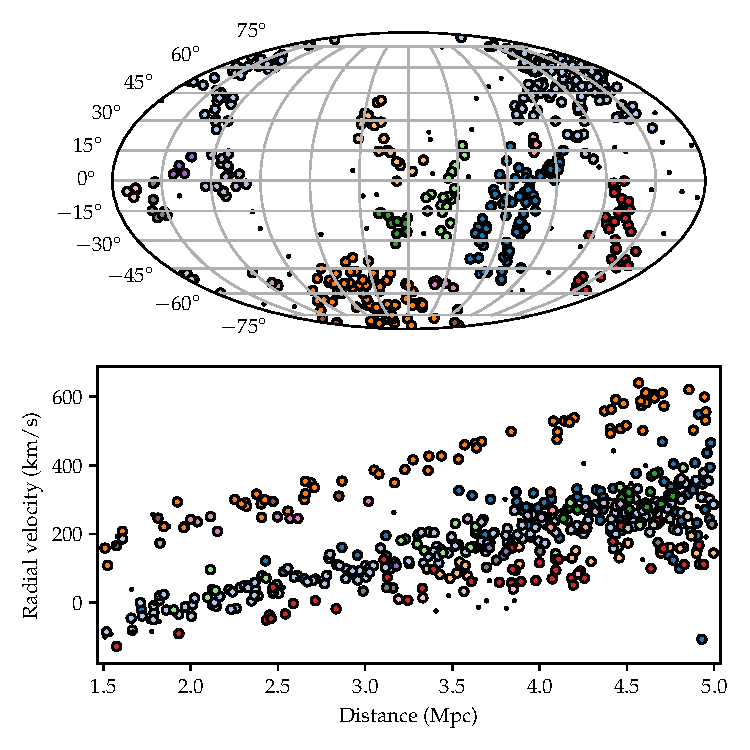
\includegraphics{kuvat/mollweide+hubble.pdf}
    \caption{TODO}\label{fig:mollweide+hubble}
\end{figure}



%\reversemarginpar
%\marginnote{\footnotesize{Massakynnys? Kaksi eri kynnystä? Liian kapea ja epätasapainoinen, laita päällekkäin?}}
Figure \ref{fig:clusteredHFparameters} shows how derived values of slope and zero-point for the Hubble flow change when the Hubble flow fitting is carried out on partial data chosen based on the cluster membership of the haloes.

\begin{figure}
    \centering
    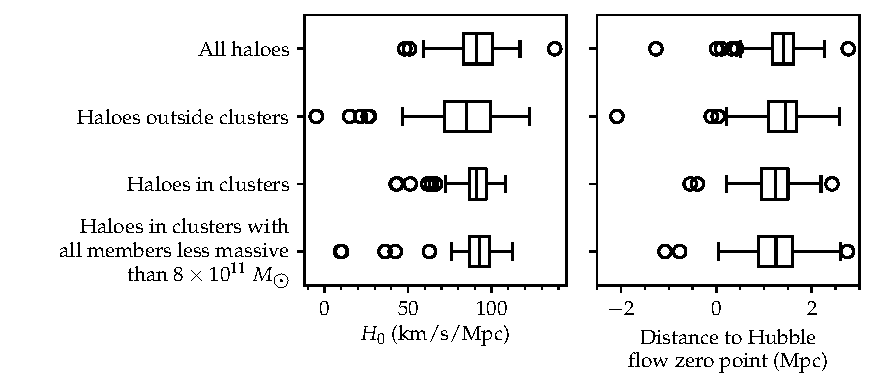
\includegraphics{kuvat/clusteredHFparameters.pdf}
    \caption{Hubble constant and distance to the point at which velocity due to the fitted Hubble flow is zero calculated from different samples. HUOM OBS NB sim 299 excluded, }\label{fig:clusteredHFparameters}
\end{figure}
%% Outliers without 299 (current case):
%allZeros: []
%inClusterZeros: []
%outClusterZeros: [-8.0111344090876742, 13.948152600724681, -4.6546938793249391]
%massCutZeros: [-6.9895372252628576, -5.8619018046506826]
%% Outliers with 299 (alternative):
%allZeros: [-30.243003145562845]
%inClusterZeros: [18.737324729385747]
%outClusterZeros: [-8.0111344090876742, 13.948152600724681, -4.6546938793249391]
%massCutZeros: [-6.9895372252628576, -5.8619018046506826]



\section{Statistical Estimate of the Local Group Mass}\label{sect:statistical_estimate}
Analysis similar to Fattahi et al 2016 paper



%\chapter{SIBELIUS project}
% Simulations Beyond the Local Universe
%
%\section{Hubble Flow Fitting}
%
% %if results
%\chapter{Conclusions}

\chapter{Conclusions}





% STEP 5:
% Uncomment the following lines and set your .bib file and desired bibliography style
% to make a bibliography with BibTeX.
% Alternatively you can use the thebibliography environment if you want to add all
% references by hand.

\clearpage
\addcontentsline{toc}{chapter}{Bibliography} % This lines adds the bibliography to the ToC
\bibliographystyle{plainnat}
\bibliography{lahteet}

\newpage
\appendix
\chapter{Principal Components}

\begin{table}
	\centering
	\rotatebox{90}{
	\begin{tabular}{l | l | l l l | l l l | l l l}
      \thead{PC} & \thead{$H_0$} & \thead{HF zero} & \thead{HF zero\\(clustered)} & \thead{HF zero\\(not clustered)} & \thead{$\sigma_{radvel}$} & \thead{$\sigma_{radvel}$\\(clustered)} & \thead{$\sigma_{radvel}$\\(not clustered)} & \thead{$v_{r, LG}$} & \thead{$v_{t, LG}$} & \thead{$r_LG$}\\
      \hline
	\makecell{1} & \makecell{-0.386} & \makecell{-0.449} & \makecell{-0.324} & \makecell{-0.379} & \makecell{-0.393} & \makecell{-0.211} & \makecell{-0.384} & \makecell{-0.211} & \makecell{0.097} & \makecell{0.013}\\
	\makecell{2} & \makecell{0.147} & \makecell{0.221} & \makecell{0.248} & \makecell{0.150} & \makecell{-0.064} & \makecell{-0.599} & \makecell{-0.056} & \makecell{-0.599} & \makecell{-0.103} & \makecell{0.332}\\
	\makecell{3} & \makecell{0.287} & \makecell{0.145} & \makecell{0.186} & \makecell{0.223} & \makecell{-0.531} & \makecell{0.258} & \makecell{-0.535} & \makecell{0.258} & \makecell{0.115} & \makecell{0.313}\\
	\makecell{4} & \makecell{0.009} & \makecell{0.020} & \makecell{-0.152} & \makecell{0.102} & \makecell{0.151} & \makecell{-0.047} & \makecell{0.136} & \makecell{-0.047} & \makecell{0.934} & \makecell{0.221}\\
	\makecell{5} & \makecell{-0.024} & \makecell{-0.171} & \makecell{-0.273} & \makecell{-0.105} & \makecell{0.140} & \makecell{0.134} & \makecell{0.227} & \makecell{0.134} & \makecell{-0.270} & \makecell{0.840}\\
	\makecell{6} & \makecell{0.015} & \makecell{-0.092} & \makecell{0.706} & \makecell{-0.663} & \makecell{0.049} & \makecell{0.065} & \makecell{0.072} & \makecell{0.065} & \makecell{0.147} & \makecell{0.127}\\
	\makecell{7} & \makecell{-0.848} & \makecell{0.156} & \makecell{0.323} & \makecell{0.343} & \makecell{-0.074} & \makecell{0.071} & \makecell{0.060} & \makecell{0.071} & \makecell{-0.001} & \makecell{0.128}\\
	\makecell{8} & \makecell{-0.162} & \makecell{0.582} & \makecell{-0.206} & \makecell{-0.315} & \makecell{0.456} & \makecell{0.024} & \makecell{-0.529} & \makecell{0.024} & \makecell{-0.018} & \makecell{0.061}\\
	\makecell{9} & \makecell{0.041} & \makecell{-0.572} & \makecell{0.239} & \makecell{0.326} & \makecell{0.549} & \makecell{-0.008} & \makecell{-0.452} & \makecell{-0.008} & \makecell{-0.016} & \makecell{0.031}\\
	\makecell{10} & \makecell{0.000} & \makecell{-0.000} & \makecell{0.000} & \makecell{0.000} & \makecell{-0.000} & \makecell{0.707} & \makecell{-0.000} & \makecell{-0.707} & \makecell{0.000} & \makecell{-0.000} 
	\end{tabular}
	}
	\caption{component	H0s	zeropoints	inClusterZeros	outClusterZeros	allDispersions	clusterDispersions	unclusteredDispersions	radialVelocities	tangentialVelocities	LGdistances
}\label{tab:PCs}
\end{table}

\end{document}

